% Format teze zasnovan je na paketu memoir. Prilikom
% zadavanja klase memoir, navedenim opcijama se podešava
% veličina slova (12pt) i jednostrano štampanje (oneside).
\documentclass[12pt,oneside]{memoir}

% Paket koji definiše sve specifičnosti mastera Matematičkog fakulteta
\usepackage{matfmaster}

% Paket koji obezbeđuje ispravni prikaz ćiriličkih italik slova
\usepackage{cmsrb}

% Ostali paketi koji se koriste u dokumentu
\usepackage{amsmath} % matematika (matrice)
\usepackage{CJKutf8} % japanski jezik (CJK)
\usepackage[ruled]{algorithm2e} % algoritmi
\usepackage{nicematrix} % lepe matrice (mape)
\usepackage[strings]{underscore} % donja crta
\usepackage{hhline} % lepa horizontalna linija
\usepackage{float} % precizno pozicioniranje
\usepackage[labelfont=bf]{caption} % bold

% Učitavanje slika iz posebnog direktorijuma
\graphicspath{{../slike}}

% Komanda za ispis (npr. caption) u dva reda
\newcommand{\dvareda}[2][c]{\begin{tabular}[#1]{@{}c@{}}#2\end{tabular}}

% Komanda za rad sa problemima na srpskom
\newenvironment{problem}[1][!ht]
{\renewcommand{\algorithmcfname}{Проблем}
\begin{figure}[!ht]
\centering
  \begin{minipage}{.94\linewidth}
	\begin{algorithm}[#1]%
  }{\end{algorithm}
  \end{minipage}
\end{figure}}

% Komanda koja prvi algoritam označava kao nulti
\setcounter{algocf}{-1}

% Datoteka sa literaturom u BibTex tj. BibLaTeX/Biber formatu
\bib{HMM-u-bioinformatici}

% Ime kandidata na srpskom jeziku (u odabranom pismu)
\autor{Лазар М. Васовић}
% Naslov teze na srpskom jeziku (u odabranom pismu)
\naslov{Скривени Марковљеви модели у биоинформатици -- електронска лекција}
% Godina u kojoj je teza predana komisiji
\godina{2021}
% Ime i afilijacija mentora (u odabranom pismu)
\mentor{др Јована \textsc{Ковачевић}, доцент\\ Универзитет у Београду, Математички факултет}
% Ime i afilijacija prvog člana komisije (u odabranom pismu)
\komisijaA{... ... \textsc{...}, ...\\ ..., ...}
% Ime i afilijacija drugog člana komisije (u odabranom pismu)
\komisijaB{... ... \textsc{...}, ...\\ ..., ...}
% Datum odbrane (obrisati ili iskomentarisati ako nije poznat)
\datumodbrane{септембар 2021.}

% Apstrakt na srpskom jeziku (u odabranom pismu)
\apstr{%
Скривени Марковљеви модели (\textit{HMM}) могу се врло упрошћено схватити као стохастички коначни аутомати са приватним (скривеним) стањима и јавним (опсервабилним) емисијама. Промене стања, које граде скривене путеве, као и приказ симбола, који чине опажања, заправо су два повезана статистичка процеса, чији се однос моделује. Примене ових модела су разнородне, како у решавању проблема надгледаног, тако и ненадгледаног машинског учења над секвенцијалним подацима, попут класификације протеина и проналажења гена у биоинформатици. Управо су ова два важна биолошка проблема описана у уводном делу рада, а објашњен је и додатни мотивациони проблем непоштене коцкарнице. У наставку су на уведеном примеру казина детаљно описане могућности скривених Марковљевих модела, попут декодирања (одређивања највероватнијег скривеног пута на основу опаженог исхода) и израчунавања вероватноће опажања. Након тога, приказано је како се дефинисани модел може искористити за решавање изложених проблема, конкретно проналажењем \textit{CG} острва (\textit{CpG} места) и употребом профилних \textit{HMM} (\textit{HMM} профила), који су такође дефинисани у тексту. Напослетку је описана и могућност учења параметара модела на основу опажања. У оквиру рада на теми, направљена је електронска лекција, као суштински најзначајнији допринос. Лекција је реализована у виду \textit{Jupyter} свеске са \textit{Python} кодовима, која је јавно доступна на \textit{GitHub}-у. У свесци су имплементирани сви изложени алгоритми, а направљена је и \textit{HTML} верзија материјала исте садржине, како би лекцију могао да погледа свако са прегледачем веба.
}

% Ključne reči na srpskom jeziku (u odabranom pismu)
\kljucnereci{биоинформатика, скривени Марковљеви модели ({\small\textit{HMM}}), електронска лекција, \textit{CG} острва ({\small\textit{CpG} места}), профилни \textit{HMM} ({\small\textit{HMM} профили)}}

\begin{document}
\begin{CJK}{UTF8}{ipxm}
% ====================================================================
% Uvodni deo teze
\frontmatter
% ====================================================================
% Naslovna strana
\naslovna
% Strana sa podacima o mentoru i članovima komisije
\komisija
% Strana sa podacima o disertaciji na srpskom jeziku
\apstrakt
% Sadržaj teze
\tableofcontents*

% ====================================================================
% Glavni deo teze
\mainmatter
% ====================================================================

% ------------------------------------------------------------------------------
\chapter{Увод}
% ------------------------------------------------------------------------------
Биоинформатика је интердисциплинарна област која се бави применом рачунарских технологија у области биологије и сродних наука, са нагласком на разумевању биолошких података. Кључна особина јој је управо поменута мултидисциплинарност, која је илустрована дијаграмом са слике \ref{fig:venn}.

\begin{figure}[H]
  \centering
  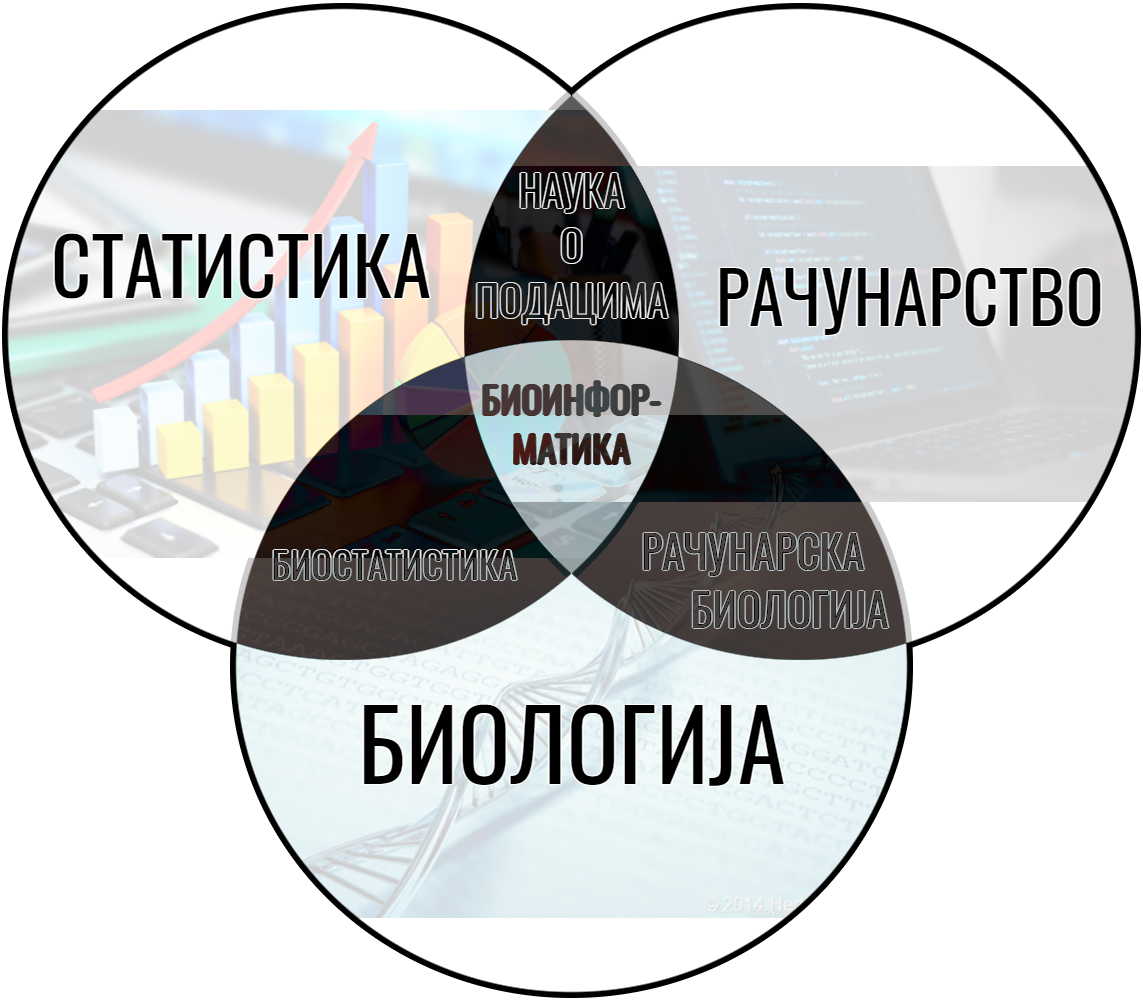
\includegraphics[width=.75\textwidth]{bioinformatika.png}
  \caption{Венов дијаграм интердисциплинарности \cite{venn}}
  \label{fig:venn}
\end{figure}

Овако представљена, биоинформатика је заправо спој статистике, рачунарства и биологије -- сва три истовремено -- по чему надилази појединачне спојеве: биостатистику, науку о подацима и рачунарску биологију. Конкретно, статистички (математички) апаратат служи за рад са подацима, рачунарске технологије тај апарат чине употребљивијим, док биологија даје потребно доменско знање (разумевање) за рад са биолошким и сродним подацима. Иако се може рећи да је биоинформатика, у савременом смислу представљеном приказаним дијаграмом, релативно млада наука, брзо је постала популарна и многи су јој посветили пажњу или се њоме баве \cite{ufpr, cmero2015, fauziyyah2019}.

Скривени Марковљев модел (у наставку углавном скраћено \textit{HMM}енгл. \textit{Hidden Markov Model}), укратко, представља статистички модел који се састоји из следећих елемената: скривених стања ($x_i$), опсервација ($y_i$), вероватноћа прелаза ($a_{ij}$), полазних ($\pi_i$) и излазних вероватноћа ($b_{ij}$), по примеру са слике \ref{fig:hmm}. \textit{HMM} се тако може схватити као коначни аутомат, при чему стања задржавају уобичајено значење, док вероватноће прелаза описују колико се често неки прелаз реализује. Полазне вероватноће одређују почетно стање. Овакав аутомат допуњује се идејом да свако стање са одређеном излазном вероватноћом емитује (приказује) неку опсервацију. Штавише, најчешће су само опажања и позната у раду са \textit{HMM}, док се позадински низ стања погађа ("предвиђа"), па се управо зато стања и модели називају скривеним \cite{stamp2021}.

\begin{figure}[H]
  \centering
  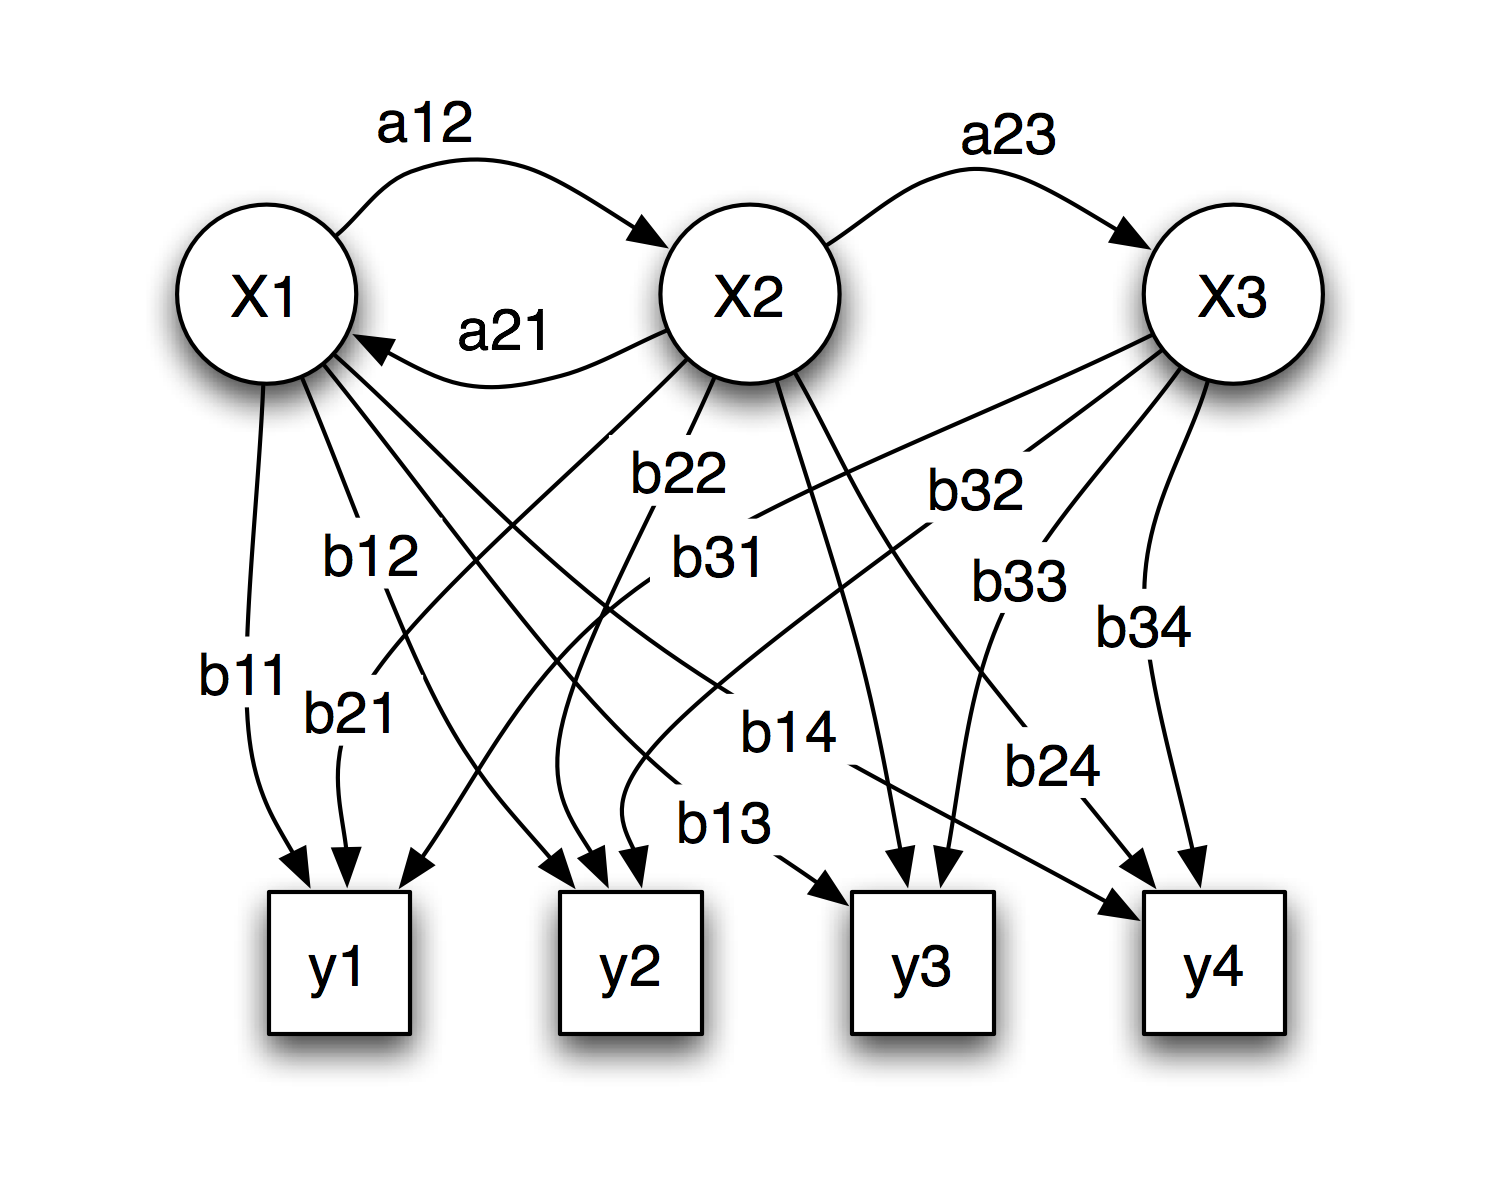
\includegraphics[width=.74\textwidth]{hmm.png}
  \caption{Једноставан пример скривеног Марковљевог модела \cite{hmm}}
  \label{fig:hmm}
\end{figure}

Циљ овог рада је спајање претходно уведених појмова -- биоинформатике и скривених Марковљевих модела. Замисао је, дакле, детаљна обрада теоријских и практичних аспеката \textit{HMM}, као и приказ примера њихове примене у биоинформатици. Поред писаног рада, предвиђена форма је и електронска лекција, која би касније била део ширег електронског уџбеника из биоинформатике. Идеја уџбеника је да буде комплетно наставно средство из ове области, које се може користити у разним облицима наставе (предавања, вежбе), али и за припрему испита или једноставно упознавање са појмом \textit{HMM}. 

Излагање је засновано на књизи \textit{Bioinformatics Algorithms: An Active Learning Approach} \cite{compeau2015} аутора Филипа Компоа (\textit{Phillip Compeau}) и Павела Певзнера (\textit{Pavel Pevzner}), која се користи као уџбеник на више од сто светских факултета \cite{ba}, међу којима је и Математички факултет Универзитета у Београду \cite{matf}. У тексту су објашњени, а у лекцији и имплементирани, сви алгоритми који су представљени у књизи, али и многи други. Резултат је \textit{Jupyter} свеска са \textit{Python} кодовима, која је јавно доступна на \textit{GitHub}-у \cite{vasovich2021}.

% ------------------------------------------------------------------------------
\chapter{Мотивација}
% ------------------------------------------------------------------------------
У овој глави изложена је мотивација за употребу скривених Марковљевих модела у биоинформатици. Конкретно, представљена су два важна биолошка проблема која се њима могу решити и пратећи појмови из домена, као и једна историјски мотивисана вероватносна мозгалица.

% Classifying the HIV Phenotype
\section{Погађање фенотипа}
ХИВ је вирус хумане имунодефицијенције, један од најпознатијих вируса, који заражава људе широм света. Својим дугорочним деловањем доводи до смртоносног синдрома стечене имунодефицијенције, познатијег као сида или \textit{AIDS}. Мада поједини аутори распрострањеност ХИВ-а називају пандемијом, Светска здравствена организација означава је као "глобалну епидемију" \cite{who}.

Постојање ХИВ-а званично је потврђено почетком осамдесетих година двадесетог века, мада се претпоставља да је са примата на људе прешао знатно раније. Недуго по овом открићу, тачније 1984, из америчког Министарства здравља и услуга становништву најављено је да ће вакцина бити доступна кроз наредне две године. Готова вакцина, међутим, ни данас није доступна, а многи покушаји су отказани након што се испоставило да кандидати чак повећавају ризик од инфекције код појединих испитаника.

Антивирусне вакцине најчешће се праве од површинских протеина вируса на који се циља, у нади да ће имунски систем, након вакцине, у контакту са живим вирусом знатно брже препознати протеине омотача вируса као стране и уништити их пре него што се вирус намножи у телу. ХИВ је, међутим, карактеристичан по томе што врло брзо мутира, па су његови протеини изузетно варијабилни и није лако научити имунски систем да исправно одреагује на све мутације. Штавише, може се десити да имунитет научи да исправно реагује само на једну варијанту вируса, а да реакција нема ефекта на остале варијанте. Овакав имунитет је лошији од имунитета који ништа не зна о вирусу, пошто не покушава да научи ништа ново, што је разлог већ поменуте ситуације да су код неких испитаника вакцине кандитати повећали ризик од заразе. Да ствар буде гора, ХИВ брзо мутира и унутар једне особе, тако да је разлика у узорцима узетих од различитих пацијената увек значајна.

Када се све узме у обзир, као обећавајућа замисао за дизајн свеобухватне вакцине намеће се следећа идеја: идентификовати неки пептид који садржи најмање варијабилне делове површинских протеина свих познатих сојева ХИВ-а и искористити га као основу вакцине. Ни то, међутим, није решење, пошто ХИВ има још једну незгодну способност: уме да се сакрије процесом гликозилације. Наиме, протеини омотача су махом гликопротеини, што значи да се након превођења за њих могу закачити многобројни гликански (шећерни) ланци. Овим процесом долази до стварања густог гликанског штита, који омета имунски систем у препознавању вируса. Све досад изнето утиче на немогућност прављења прикладне вакцине у скоријем времену.

Чак и ван контекста вакцине, мутације ХИВ-а прилично су занимљиве за разматрање. Конкретно, илустративно је бавити се \textit{env} геном, чија је стопа мутације 1--2 \% по нуклеотиду годишње. Овај ген кодира два релативно кратка гликопротеина који заједно граде шиљак (спајк) омотача, део вируса задужен за улазак у људске ћелије. Мање важан део шиљка је гликопротеин \textit{gp41} ($\sim$ 345 аминокиселина), док је важнији гликопротеин \textit{gp120} ($\sim$ 480 аминокиселина). О варијабилности другог говори чињеница да на нивоу једног пацијента, у кратком року, скоро половина аминокиселина буде измењена позадинским мутацијама одговарајућег гена, као да је сасвим други протеин.

Проблематика је још занимљивија када се, поред генотипа вируса, разматра и његов фенотип. На примеру ХИВ-а, након уласка у људску ћелију, гликопротеини омотача код неких изолата могу да изазову спајање заражене ћелије са суседним ћелијама. Резултат тога је синцицијум -- нефункционална вишеједарна ћелијска (цитоплазматична) маса са заједничком ћелијском мембраном. Према тој могућности сваки конкретни вирус може се означити као изолат који ствара синцицијум или као изолат који га не ствара. Прва група се тим процесом знатно брже умножава, што даље значи да је опаснија и агресивнија, јер уласком у само једну ћелију убија многе друге у суседству. Одређивање тачног генотипа и погађање фенотипа важно је како би се пацијенту преписао најприкладнији коктел антивирусних лекова.

Испоставља се да је примарна структура гликопротеина \textit{gp120} важан суштински генотипски предиктор фенотипа ХИВ-а. Наиме, узимајући у обзир само низ аминокиселина које чине \textit{gp120}, може се направити једноставан класификатор који погађа да ли проучавани изолат ствара синцицијум или не. Конкретно, научник Жан Жак де Јонг је 1992. анализирао вишеструко поравнање такозване \textit{V3} петље, издвојеног региона у оквиру \textit{gp120}, и формулисао правило 11/25 \cite{jong1992}. Према том правилу, сој ХИВ-а највероватније ствара синцицијум уколико му се на 11. или 25. позицији у \textit{V3} петљи налазе аминокиселине аргинин (\textit{R}) или лизин (\textit{K}). Пример мотива \textit{V3} петље дат је на слици \ref{fig:motif}. Приметно је да су управо 11. и 25. позиција међу најваријабилнијим, те да удео критичних \textit{R} и \textit{K} на њима није претерано велик. Наравно, на фенотип утичу и многе друге позиције унутар \textit{gp120} и других протеина.

\begin{figure}[H]
  \centering
  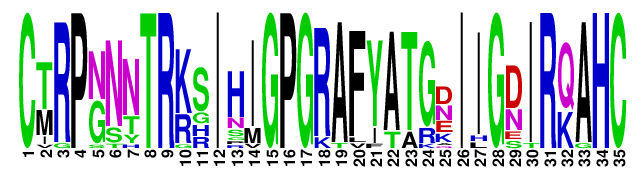
\includegraphics[width=.75\textwidth]{motif.png}
  \caption{Мотив \textit{V3} петље из књиге \cite{compeau2015} генерисан алатом \textit{WebLogo} \cite{weblogo}}
  \label{fig:motif}
\end{figure}

За крај и поенту уводног излагања о ХИВ-у, остаје неразрешен још један веома значајан проблем. Како би се уопште разматрало предвиђање фенотипа на основу примарне структуре \textit{gp120}, неопходно је прво доћи до прецизног вишеструког поравнања различитих секвенци аминокиселина. Прво, поравнање мора бити хируршки прецизно, јер нпр. само једна грешка доводи до погрешног податка која вредност је на 11. и 25. позицији \textit{V3} петље. Следеће, неопходно је адекватно обрадити инсерције и делеције, што су врло честе мутације ХИВ-а у многим регионима генома. На крају, потребно је на прави начин оценити квалитет поравнања, нпр. коришћењем различитих матрица скора за сваку појединачну позицију. Ово је донекле могуће решити једноставним алгоритмима за поравнање секвенци, попут оног за израчунавање едит растојања, али уз два главна проблема: овакви алгоритми динамичког програмирања су често велике сложености и са мање слободе код скорова, а притом не пресликавају најбоље суштину биолошког проблема класификације фенотипа у алгоритамски проблем (недостају кораци након поравнања). Постоји, дакле, потреба за новом формулацијом која обухвата све што је потребно за статистички потковано поравнање секвенци.

% Finding CG-Islands
\section{Потрага за генима}
Познато је да геном чини тек мали део ДНК секвенце. Другим речима, ДНК добрим делом не кодира протеине. Стога је један од важних биолошких проблема управо проналажење места на којима се гени налазе. Прецизније, тражи се место где њихово преписивање (транскрипција) започиње.

Почетком двадесетог века, Фибус Левин открио је да ДНК чине четири нуклеотида \cite{levene1910}, чији су главни део азотне базе: аденин (\textit{A}), цитозин (\textit{C}), гуанин (\textit{G}) и тимин (\textit{T}). У то време, међутим, није била позната тачна структура наследног материјала, штo је двострука завојница, коју су пола века касније открили Вотсон и Крик \cite{watson1953}. Левин је, стога, сматрао да ДНК носи информације једнаке било којој четворословној азбуци, а додатно и да је удео сваког од четири нуклеотида једнак. Занимљивост је да овај упрошћени модел одговара стању у савременој биоинформатици -- ДНК се углавном и посматра као секвенца нуклеотида, односно ниска над азбуком \{\textit{A}, \textit{C}, \textit{G}, \textit{T}\}.

Открићем тачне структуре допуњена је теза о једнаком уделу нуклеотида. Како су нуклеотиди на супротним ланцима упарени, њихов удео јесте врло сличан када се посматра целокупна ДНК. То, међутим, није случај када се посматра само један ланац, што је уобичајено у генетици и биоинформатици. Примера ради, удео гуанина и цитозина, који чине један базни пар, код људи је 42 \%, што је ипак статистички значајно мање од пола. На вишем нивоу гранулације, у случају да се посматрају само по две суседне базе, испоставља се да динуклеотиди \textit{CC}, \textit{CG}, \textit{GC}, \textit{GG} узимају сасвим различите уделе. Конкретно, иако би се очекивало да, под претпоставком равномерне расподеле, сваки од њих узима удео 4--5 \%, динуклетид \textit{CG} чини само 1 \% људског генома. Све ово значи да је ДНК секвенца ипак нешто даље од случајне.

Поставља се питање зашто је удео \textit{CG} тако мали. Одговор, међутим, није комплексан, поготову ако се додатно примети да је удео \textit{TG} нешто виши од очекиваног, а посебно у регионима у којима је удео \textit{CG} изразито мали. Разлог томе лежи у метилацији, најчешћој измени која природно настаје унутар ДНК. Поједини нуклеотиди, наиме, могу бити нестабилни, па се на њих лако накачи метил група ($CH_3$). Међу најнестабилнијим управо је цитозин иза ког следи гуанин, дакле \textit{C} из \textit{CG}. Метиловани цитозин даље се често спонтано деаминује у тимин, чиме динуклеотид \textit{CG} лако постаје \textit{TG}. Свеукупни резултат је да се \textit{CG} глобално појављује веома ретко, а \textit{TG} нешто чешће.

Метилација мења експресију суседних гена. Експресија оних гена чији су нуклеотиди у великој мери метиловани често је потиснута. Иако је сам процес метилације важан у току ћелијске диференцијације -- доприноси неповратној специјализацији матичних ћелија -- она углавном није пожељна у каснијем добу. Хиперметилација гена повезана је са различитим врстама рака. Стога је метилација врло ретка око гена, што значи да је на тим местима \textit{CG} знатно чешће. Овакви делови ДНК називају се \textit{CG} острвима или \textit{CpG} местима. Разлика у уделу динуклеотида у некодирајућим и регионима богатим генима дата је кроз табелу \ref{tab:cg}, која је дата директно у наставку.

\begin{table}[h!]
  \centering
  \caption{\dvareda{Удео динуклеотида у једном ланцу људског \textit{X} хромозома\\-- лево у регионима \textit{CG} острва, а десно ван њих \cite{compeau2015};\\ разлика у уделу \textit{CG} наглашена је црвеном бојом}}
  \begin{tabular}{| c | c c c c | c c c c |} \hline
   & A & C & G & T & A & C & G & T \\ \hline
  A & 0,053 & 0,079 & 0,127 & 0,036 & 0,087 & 0,058 & 0,084 & 0,061 \\
  C & 0,037 & 0,058 & \textcolor{red}{0,058} & 0,041 & 0,067 & 0,063 & \textcolor{red}{0,017} & 0,063 \\
  G & 0,035 & 0,075 & 0,081 & 0,026 & 0,053 & 0,053 & 0,063 & 0,042 \\
  T & 0,024 & 0,105 & 0,115 & 0,050 & 0,051 & 0,070 & 0,084 & 0,084 \\ \hline
  \end{tabular}
  \label{tab:cg}
\end{table}

Закључак је, дакле, да се проблем потраге за генима може свести на проналажење \textit{CG} острва. Наиван приступ потрази је употреба клизећег прозора. Узима се прозор фиксне величине и помера кроз ДНК секвенцу. Прозори (позиције прозора) са натпросечним уделом \textit{CG} јесу кандидати за \textit{CG} острва. Остаје, међутим, питање како одредити добру величину прозора, али и шта радити када преклапајући прозори (клизећи прозори који садрже исте поднизове) нуде различиту класификацију подниза. И овде би корисније било статистички потковано решење, које би отклонило наведене недоумице.

% Gambling with Yakuza
% Two Coins up the Dealer’s Sleeve
\section{Коцкање са јакузама}
Јакузе су припадници истоимене криминалне организације, традиционалног синдиката организованог криминала. Савремене јакузе потичу од јапанских путујућих коцкара, који су били распрострањени у осамнаестом веку. Једна од најпознатијих игара коју су путујући коцкари организовали у својим импровизованим коцкарницама био је чо-хан (јап. 丁半, \textit{chō-han}), у дословном преводу "пар-непар" \cite{fletcher2017}. Игра је сасвим једноставна -- претеча јакуза (крупије) баца две коцкице, док се играчи кладе да ли ће збир бити паран или непаран. Игра је такође поштена -- једнако се остварују оба исхода парности.

До занимљивог тренутка долази када се из било ког разлога осетно више играча опклади на један од два могућа резултата. Тада би имало смисла да похлепни крупије, у жељи да заради (он узима проценат зараде победника), баца отежане коцкице, које ће са већом вероватноћом дати резултат који је добио мање опклада. Једноставности ради, уместо чо-хана је у наставку разматрана нешто простија игра бацања новчића. У њој крупије баца новчић, а играчи се кладе да ли ће пасти писмо или глава. Она је знатно лакша за анализу, а суштина је иста и доводи до статистички поткованог решења у претходним поднасловима изложених биолошких и сродних проблема.

Крупијева превара у овом случају могла би бити употреба отежаног новчића, код кога исходи нису равномерно расподељени. Нека је познато да крупије има два новчића: један праведан и један отежан тако да на главу пада трипут чешће него на писмо. Циљ је за одређени низ исхода одредити да ли је настао бацањем праведног или отежаног новчића. Пажљивијом анализом проблема, испоставља се да је питање вара ли крупије лоше формулисано. Наиме, оба новчића могу да произведу било који низ исхода, па тако нпр. и отежани новчић може константно да пада на писмо. Иако дефинитивно није могуће са сигурношћу утврдити који је новчић коришћен, могуће је нешто слично и често довољно добро -- одредити који је вероватније коришћен.

Конкретно, нека је упитни новчић бачен одређени број пута, при чему је добијен низ исхода. Вероватноће исхода ($H$ од енгл. \textit{heads} -- глава и $T$ од енгл. \textit{tails} -- писмо) код праведног ($F$ од енгл. \textit{fair} -- фер) и отежаног ($B$ од енгл. \textit{biased} -- пристрасан) новчића могу се исказати следећим формулама: $$P\{H | F\} = P\{T | F\} = \frac{1}{2}, P\{H | B\} = \frac{3}{4}, P\{T | B\} = \frac{1}{4}.$$ Како су бацања независни догађаји -- претходни исходи ни на који начин не утичу на наредне -- вероватноћа да $n$ бацања произведе низ исхода $x = x_1...x_n$, од којих је пало $k$ глава, јесте производ појединачних вероватноћа: $$P\{x\} = \prod_{i=1}^n P\{x_i\} = P\{H\}^k \cdot P\{T\}^{n-k}.$$ Због тога вероватноћа сваког низа исхода код праведног новчића износи: $$P\{x | F\} = \left(\frac{1}{2}\right)^k \left(\frac{1}{2}\right)^{n-k} = \frac{1}{2^n}.$$ С друге стране, вероватноћа низа исхода код отежаног новчића је: $$P\{x | B\} = \left(\frac{3}{4}\right)^k \left(\frac{1}{4}\right)^{n-k} = \frac{3^k}{4^n}.$$

Уколико је $P\{x | F\} > P\{x | B\}$, онда је вероватније да је крупије бацао праведни новчић, док је у случају $P\{x | F\} < P\{x | B\}$ бацао отежани. Занимљиво је напоменути да ипак није лако израчунати бројеве $1/2^n$ и $3^k/4^n$ за велико $n$. Они су тада изразито мали, па је питање да ли би били добро представљени у рачунару, те да ли њихово поређење даје тачан резултат. Стога се израчунава логаритамски однос вероватноћа, који у конкретном случају износи: $$\log_2\left(\frac{P\{x | F\}}{P\{x | B\}}\right) = \log_2\left(\frac{2^n}{3^k}\right) = n - k\log_23.$$ Овај број се већ без проблема израчунава и представља у рачунару. Конкретно, нека је $n = 100$ (сто бацања), а $k = 63$ (нешто већи удео глава). Тада је логаритамски однос приближно једнак 0,15. Позитивна вредност $\log(x/y)$ значи да је $x/y > 1$, односно $x > y$ у случају ненегативних вероватноћа. Ово значи да је већа вероватноћа да је крупије бацао праведни новчић, иако је $k = 63$ интуитивно и по апсолутној вредности ближе $3/4 \cdot 100 = 75$ него $1/2 \cdot 100 = 50$. Негативан логаритамски однос довео би до супротног закључка. Алтернативно, како је неопходно одредити само знак израза $n - k\log_23$, то се може учинити поређењем $n$ и $k\log_23$, односно $k/n =$ 0,63 и $1/\log_23 \approx$ 0,6309 након дељења $k$ са обе стране. Лева страна је мања, па је однос позитиван.

Изложени вероватносни модел игре пада у воду када се узме у обзир могућност да крупије наизменично баца праведни и отежани новчић. Наиме, искусни преварант могао би да смањи сумњу да користи отежани новчић тако што би га понекад -- додуше, ретко, како не би био ухваћен -- заменио са праведним, и тако укруг. Поставља се питање како само на основу низа исхода и евентуално познате вероватноће промене новчића након сваког бацања одредити када је бачен праведни, а када отежани новчић. И овога пута, одговор може бити само несигурног типа -- који новчић је када вероватније коришћен.

Слично као код проблема проналажења \textit{CG} острва, потребно је на неки начин различите секвенце новчића упоредити и одредити која је бољи одговор на постављено питање. И овде би наивно решење подразумевало употребу клизајућег прозора који би пролазио кроз све поднизове бацања. На нивоу прозора могли би се рачунати логаритамски односи, према којима би се даље одредило порекло прозора -- позитиван однос сугерише да је прозор настао бацањем праведног новчића и супротно. Овакав приступ занемарује тачну вероватноћу замене новчића, мада имплицитно узима у обзир да је она мала.

Остају, међутим, већ поменути проблеми са прозорским приступом: како одредити добру величину прозора, као и шта радити када преклапајући прозори нуде различиту класификацију подниза. Примера ради, ако крупије наизменично баца два претходно описана новчића, а добијени низ исхода је $x = HHHHHTTHHHTTTTT$, онда прозор $x_1...x_{10} = HHHHHTTHHH$ има негативан логаритамски однос, док је однос преклапајућег прозора $x_6...x_{15} = TTHHHTTTTT$ позитиван. Није јасно како одлучити који је новчић бацан у пресеку $x_6...x_{10} = TTHHH$, односно у ком тренутку је тачно дошло до замене новчића, те да ли је замене уопште и било или је крупије поштен.

Још једном је јасно да би најбоље било осмислити статистички потковано решење за све досад изложене проблеме. То је и учињено у следећем поглављу, баш са претходно изложеним бацањем новчића као прилично једноставним, али ипак сасвим интуитивним мотивационим примером.

\section{Додатни проблеми}
Досад су изложена два биолошка проблема за која је закључено да би добро било осмислити статистички потковано решење: погађање фенотипа и потрага за генима. Први се своди на класификацију геномске секвенце (нпр. ХИВ-а) на основу познатих могућих исхода и њихових примера. Други се своди на откривање \textit{CG} острва, региона ДНК са високим уделом динуклеотида \textit{CG}. Иако су ово два конкретна проблема из домена биологије, јасно је да би се жељено решење могло применити и на мноштво других сличних проблема, што укључује последњи пример са бацањем новчића.

Приметно је да је секвенцијалност главна особина података са којима се ради при решавању претходно описаних проблема. Први проблем стога се заправо лако уопштава на проблем класификације било каквих секвенцијалних података, под условом да се сличност мери на основу измена које одговарају мутацијама које настају у геному, што су супституције, инсерције и делеције. Други проблем му је сличан, с тим што класификује (заправо групише -- кластерује) поднизове једне секвенце. Кад се све узме у обзир, испоставља се да би жељено решење истовремено било корисно како за проблеме надгледаног, тако и ненадгледаног машинског учења над секвенцијалним подацима \cite{khoda2014}.

Овакво решење могло би се аналогно користити за додељивање новооткривених протеина некој постојећој фамилији \cite{nguyen2016} (класификација), моделовање и препознавање људског понашања, гестова, рукописа и говора \cite{gales2007} (класификација), обраду звука и сигнала \cite{andreao2006} (класификација и кластеровање) или одређивање врсте речи у тексту \cite{mutjaba2020}. Домен примене је чак и моделовање тока пандемије \textit{COVID-19} засновано на најосновнијим подацима, чији се пример резултата у случају Републике Србије може видети на слици \ref{fig:covid}, док се детаљније информације о моделима могу добити увидом у цитирани рад.

\begin{figure}[H]
  \centering
  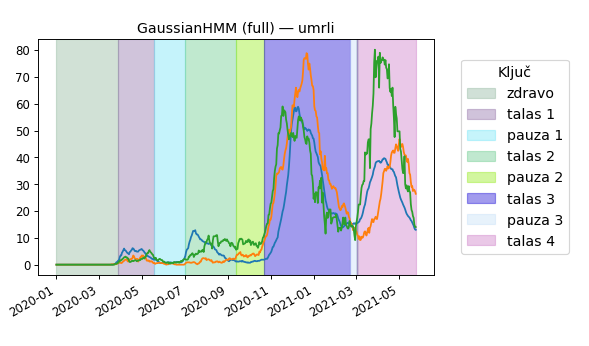
\includegraphics[width=.8\textwidth]{covid.png}
  \caption{Моделовање епидемије \textit{COVID-19} у Србији \cite{vasovic2021}}
  \label{fig:covid}
\end{figure}

Досад је више пута наговештено да су добар избор скривени Марковљеви модели. Ваља, међутим, напоменути да се многи наведени проблеми још ефектније решавају својеврсним проширењима \textit{HMM}-а, попут условних случајних поља \cite{ponomareva2007}, или комбинацијом са вештачким неуронским мрежама \cite{cohen1999}.

% ------------------------------------------------------------------------------
\chapter{Моделовање}
% ------------------------------------------------------------------------------
Након мотивације, у овој глави су дефинисани скривени Марковљеви модели, као предложено решење свих досад изложених проблема. Поред дефиниције, на примеру бацања новчића (непоштене коцкарнице) приказано је како се тачно проблеми моделују помоћу \textit{HMM}, те како се на основу тог модела може одговорити на нека важна питања.

% Hidden Markov Models (1)
\section{Дефиниција модела}
Како би се лакше конструисао општи модел за решавање свих досадашњих проблема, а посебно бацања новчића, крупије се, уместо као особа, може схватити као примитивна машина -- аутомат. Структура му за почетак није важна, али његово деловање јесте. Аутомат је секвенцијалне природе, те оперише кроз низ корака. У сваком кораку је у неком приватном стању, које означава који новчић је заправо бачен (конкретно \textit{F} и \textit{B}), при чему јавно приказује исход бацања тог новчића (конкретно \textit{H} и \textit{T}). Стање је, дакле, непознато, па се другачије назива скривеним стањем. И стања и опажања погодно је апстраховати симболима, нпр. баш карактерима, како је и учињено.

У сваком кораку, аутомат доноси две одлуке: у које скривено стање прећи (да ли га променити) и који симбол емитовати у том новом стању. Испоставља се да се обе одлуке могу донети у потпуности стохастички, што би значило да је добијен жељени статистички потковани модел проблема. Заиста, прва одлука може се донети тако што се случајно одабере \textit{F} или \textit{B} као почетно стање (нпр. баш равномерно, са једнаким вероватноћама 1/2), а надаље се у сваком кораку стање мења са неком малом вероватноћом (нпр. 1/10), док се са знатно већом преосталом (нпр. 9/10) остаје у истом стању. Друга одлука доноси се на основу прве и већ познатих вероватносних особина новчића -- нпр. вероватноћа емитовања \textit{H} једнака је 1/2 у стању \textit{F}, а 3/4 у стању \textit{B}.

Претходно изложени аутомат заправо одговара дуго најављиваном појму скривених Марковљевих модела. \textit{HMM} се традиционално представља као статистички модел који се састоји из следећих основних елемената:
\begin{itemize}
  \item скривених стања $x_i$ -- свако стање из скупа $x$ има индекс $i$,
  \item опажања, опсервација, емисија, приказа, исхода, симбола $y_i$,
  \item полазних вероватноћа $\pi_i$ -- колико је често $x_i$ почетно стање,
  \item вероватноћа прелаза $a_{ij}$ -- колико се често из $x_i$ прелази у $x_j$,
  \item излазних вероватноћа $b_{ij}$ -- колико се често у стању $x_i$ емитује $y_j$.
\end{itemize}
Пример који одговара оваквој дефиницији дат је на слици \ref{fig:hmm}. Наравно, подразумева се да су познати број стања $n$ (тако заправо $x = \{x_1, ..., x_n\}$, $\pi = \{\pi_1, ..., \pi_n\}$ и $a = \{a_{ij}\}_{1 \leq i, j \leq n}$) и број могућих опсервација $m$ (тако заправо $y = \{y_1, ..., y_m\}$ и $b = \{b_{ij}\}_{1 \leq i \leq n, 1 \leq j \leq m}$) као помоћни елементи сваког \textit{HMM}.

Како су сви скупови коначни, прецизније се говори о дискретним (мултиномијалним) \textit{HMM}, мада је иначе могуће моделовати разне непрекидне расподеле \cite{jordan2004}. Додатно, \textit{HMM} се у литератури често дефинише још простије, као уређена тројка $\{a, b, \pi\}$, односно $\{A, B, \pi\}$ ако се користе велика слова. Стварно, скупови $x$ и $y$ просто се мењају индексима, познатим из тројке.

Како би овакав модел био у потпуности статистички заснован и смислен, обично се захтева да се све појединачне вероватноће сабирају у јединицу: $$\sum_{i=1}^n \pi_i = 1, (\forall i \in \{1, ..., n\}) \sum_{j=1}^m a_{ij} = 1, (\forall i \in \{1, ..., n\}) \sum_{j=1}^m b_{ij} = 1.$$ Постоје, међутим, изузеци који су детаљније обрађени у наставку, када се говори о важним надградњама појма скривених Марковљевих модела.

На основу већ разматране слике \ref{fig:hmm}, познато је да се \textit{HMM} може илустровати \textit{HMM} дијаграмом. Ради се о графу чији су чворови стања и опсервације, а гране вероватноће преласка и емисије. Стил је у суштини произвољан, мада се на слици примећује разлика у значењу графичких елемената. Стања су приказана кружним, а емисије квадратним чворовима. Вероватноће преласка исписане су изнад грана, а излазне вероватноће на самим гранама. Прелази и емисије нулте вероватноће (нпр. прелаз са $x_1$ на $x_3$ или на самог себе) нису ни приказани. Други стилови могу приказати све гране, а емисије и вероватноће емисија означити испрекиданим линијама. Независно од стила, \textit{HMM} једнозначно одређује структуру свога дијаграма, а важи и обрнуто.

Сада је могуће искористити \textit{HMM} за прецизно моделовање проблема бацања коцкице у непоштеној коцкарници. За конкретни случај, изложен на почетку поднаслова, дијаграм је приказан на слици \ref{fig:kock}.

\begin{figure}[H]
  \centering
  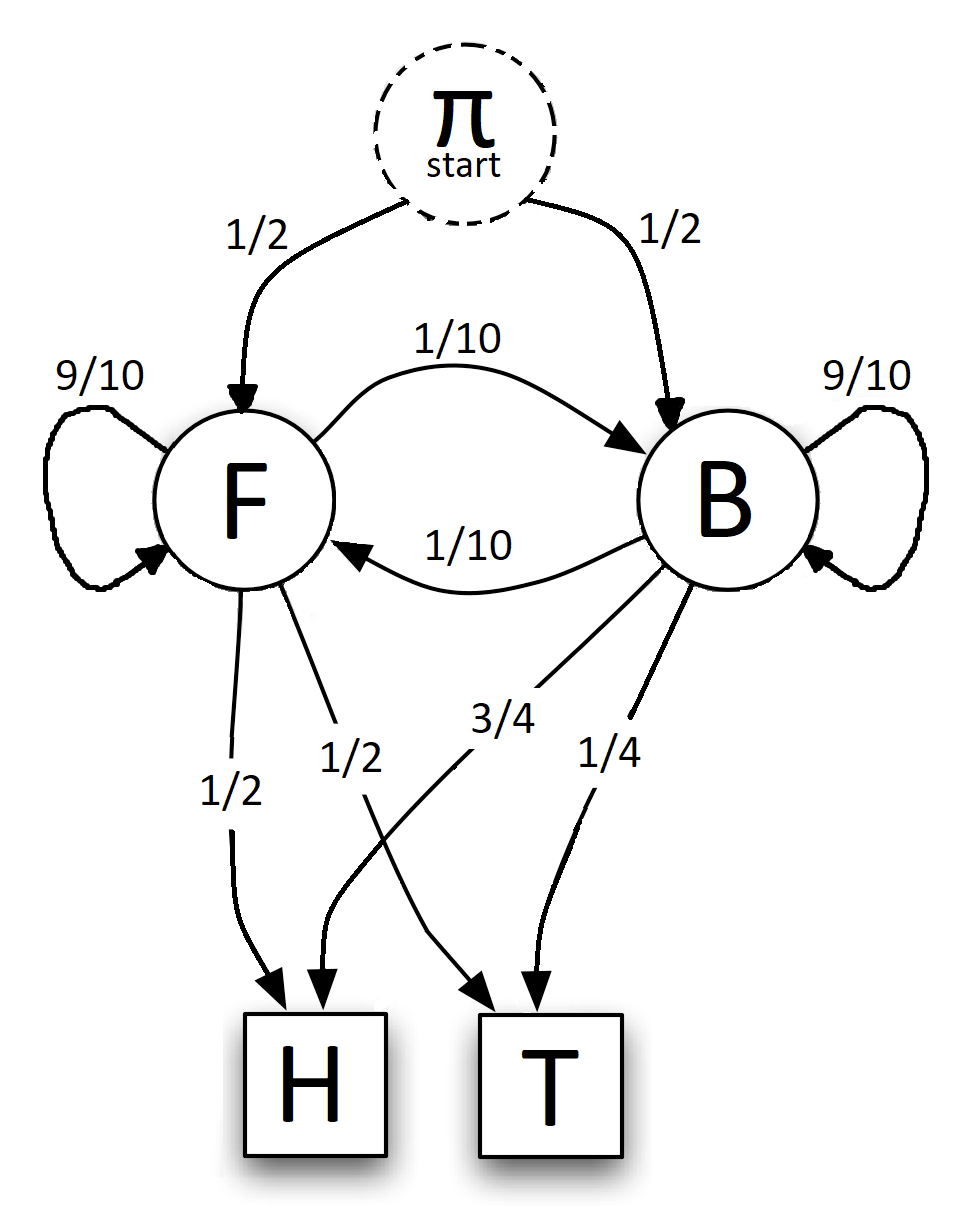
\includegraphics[width=.5\textwidth]{kockarnica.png}
  \caption{Скривени Марковљев модел бацања новчића}
  \label{fig:kock}
\end{figure}

Служи се истим стилом као претходно описани граф, с тим што додатно испрекидано приказује замишљено полазно стање, што је новина на слици. Уређена петорка изгледа овако и пружа исте информације:
\begin{itemize}
  \item скривена стања $x = \{F, B\}$ -- нпр. $x_1 = F$ и $x_2 = B$,
  \item опсервације $y = \{H, T\}$ -- нпр. $y_1 = H$ и $y_2 = T$,
  \item полазне вероватноће $\pi = \left\{\dfrac{1}{2}, \dfrac{1}{2}\right\}$ -- нпр. $\pi_1 = P\{x_1\} = P\{F\} = \dfrac{1}{2}$,
  \item преласци $a = \left(\begin{matrix}\dfrac{9}{10} & \dfrac{1}{10}\\[8pt] \dfrac{1}{10} & \dfrac{9}{10}\end{matrix}\right)$ -- нпр. $a_{12} = P\{x_1 \mapsto x_2\} = P\{F \mapsto B\} = \dfrac{1}{10}$,
  \item емисије $b = \left(\begin{matrix}\dfrac{1}{2} & \dfrac{1}{2}\\[8pt] \dfrac{3}{4} & \dfrac{1}{4}\end{matrix}\right)$ -- нпр. $b_{21} = P\{y_1 | x_2\} = P\{H | B\} = \dfrac{3}{4}$.
\end{itemize}

Историјски гледано, појам \textit{HMM} увели су Ленард Баум и сарадници кроз низ статистичких радова објављених у другој половини шездесетих година двадесетог века \cite{baum1966}. \textit{HMM} је надградња појма Марковљевих ланаца (енгл. \textit{Markov Chain, MC}), који су у суштини \textit{HMM} без емисија. Ради се, дакле, о уобичајеном стохастичком аутомату, који се састоји из стања и вероватноћа прелаза. \textit{MC} је почетком века формулисао руски статистичар Андреј Марков, по коме су и названи, како би моделовао Марковљеве процесе -- стохастичке промене стања такве да тренутно стање зависи искључиво од претходног \cite{markov1906}. Прва практична примена \textit{HMM} била је препознавање говора, док је биолошка примена почела 1986, Бишоповим и Томпсоновим поравнањем ДНК \cite{bishop1986}.

% Hidden Markov Models (2)
\section{Могућности модела}
Могуће је дефинисати појам скривеног пута $p = p_1...p_k$ као низ $k$ стања кроз која \textit{HMM} пролази, а да притом емитује секвенцу опсервација $o = o_1...o_k$. Примера ради, може бити да је низ видљивих исхода $o = THTHHHTHTTH$, а позадински низ скривених стања $p = FFFBBBBBFFF$. Главна идеја је анализирати у ком су односу $p$ и $o$, те са којом се вероватноћом реализују.

Уз излагање \textit{HMM} за бацање новчића у непоштеној коцкарници, дати су примери значења чланова петорке, који донекле наговештавају могућности скривених Марковљевих модела. Прво, напоменуто је да полазне вероватноће заправо представљају вероватноћу да се у првом кораку ушло у неко стање. Другим речима, то су заправо вероватноће $P\{p\}$ свих могућих једночланих низова скривених стања. Друго, имплицирано је да матрица емисија складишти маргиналну расподелу емисија при познатом стању. То су условне вероватноће $P\{o | p\}$ исхода при једночланом низу скривених стања.

Могуће је, дакле, директно из дефиниције \textit{HMM} израчунати вероватноће  $P\{p\}$ и $P\{o | p\}$ за $k = 1$, и то као $P\{x_i\} = \pi_i$, односно $P\{y_j | x_i\} = b_{ij}$. Према познатој формули условне вероватноће, важи $P\{p, o\} = P\{p\} P\{o | p\}$, па је и та вероватноћа тривијално позната за путеве јединичне дужине, као $P\{x_i, y_j\} = \pi_i b_{ij}$. Реч је о заједничкој вероватноћи да \textit{HMM} пролази кроз низ стања $p$, а да притом емитује управо секвенцу опсервација $o$. Према уобичајеним принципима, могуће је приметити следеће: $\sum_p \sum_o P\{p, o\} = 1$. Наиме, када се саберу вероватноће свих могућих комбинација низа опажања и скривених путева одређене дужине $k$, добија се јединица, што значи да је покривен цео простор догађаја у \textit{HMM}. Из ове дводимензионалне (заједничке) расподеле путева и емисија могу се без проблема извести маргиналне (појединачне) расподеле путева $P\{p\} = \sum_o P\{p, o\}$ и симбола $P\{o\} = \sum_p P\{p, o\}$.

Подсећања ради, оригинални циљ код непоштене коцкарнице био је пронаћи највероватнији низ стања (бачених новчића) за познати низ опсервација (исхода), што је управо максимална вредност $P\{p, o\}$ по свим $p$ за познато $o$. Претходно опште постављен задатак проналаска највероватнијег низа бацања на основу анализе исхода постаје сасвим конкретан статистички проблем -- на основу емитоване ниске симбола $o$ одредити највероватнију секвенцу скривених стања $p$. У наставку је показано како је то заправо могуће урадити.

За почетак, важно је формално дефинисати проблем. Пример наивне формулације дат је проблемом \ref{prob:kock}. За њу и њој сличне је, међутим, већ закључено да у суштини нису смислене. Зато је и уведен појам \textit{HMM}.

\begin{problem}[H]
  \SetAlgoLined
  \textit{На основу низа исхода бацања новчића, одредити када крупије у непоштеној коцкарници користи који од два могућа новчића.}\\
  \textbf{Улаз}: низ $o = o_1...o_k$ исхода ($H$ и $T$) бацања два новчића ($F$ и $B$).\\
  \textbf{Излаз}: низ $p = p_1...p_k$ новчића такав да је $o_i$ резултат бацања $p_i$.
  \caption{Непоштена коцкарница}
  \label{prob:kock}
\end{problem}

Добра формулација преко појма \textit{HMM} дата је кроз проблем \ref{prob:dekod}. Управо је она детаљно обрађена у наставку овог поглавља, као његов централни део.

\begin{problem}[H]
  \SetAlgoLined
  \textit{Пронаћи оптимални пут кроз \textit{HMM} ако је емитована ниска $o$.}\\
  \textbf{Улаз}: ниска $o = o_1...o_k$ и \textit{HMM}$\{a, b, \pi\}$ који ју је емитовао.\\
  \textbf{Излаз}: скривени пут $p$ који максимизује вероватноћу $P\{p, o\}$ над свим могућим путевима, дакле $\operatorname*{argmax}_p P\{p, o\}$ за улазно $o$.
  \caption{Декодирање приказа}
  \label{prob:dekod}
\end{problem}

Прва идеја јесте исцрпна претрага простора догађаја над маргиналном расподелом $P\{p, o\}$ за познато $o$. Стога се формулише нови проблем \ref{prob:putishod}.

\begin{problem}[H]
  \SetAlgoLined
  \textit{Израчунати вероватноћу пута и опажања у \textit{HMM}.}\\
  \textbf{Улаз}: скривени пут $p = p_1...p_k$ кроз \textit{HMM}$\{a, b, \pi\}$ и ниска $o = o_1...o_k$ која је тим проласком емитована.\\
  \textbf{Излаз}: заједничка вероватноћа пута и исхода $P\{p, o\}$.
  \caption{Вероватноћа пута и исхода}
  \label{prob:putishod}
\end{problem}

Како је $P\{p, o\} = P\{p\} P\{o | p\}$, тако је најпогодније независно израчунати $P\{p\}$ и $P\{o | p\}$ за сваки од $n^k$ скривених путева. Број путева (такође и ниски симбола) дужине $k$ у \textit{HMM} са $n$ могућих стања иначе је експоненцијалан зато што се одабир сваког своди на варијације -- уређене изборе са понављањем.

Први потпроблем је израчунавање вероватноће пута, што се може формализовати проблемом \ref{prob:put}. Он је у наставку решен у виду једне формуле.

\begin{problem}[H]
  \SetAlgoLined
  \textit{Израчунати вероватноћу скривеног пута $p$ кроз \textit{HMM}.}\\
  \textbf{Улаз}: скривени пут $p = p_1...p_k$ кроз \textit{HMM}$\{a, b, \pi\}$.\\
  \textbf{Излаз}: вероватноћа улазног пута $P\{p\}$.
  \caption{Вероватноћа скривеног пута \cite{ba10a}}
  \label{prob:put}
\end{problem}

Први елемент $P\{p\}$, дакле, представља вероватноћу скривеног пута $p$, односно вероватноћу да \textit{HMM} прође кроз низ стања $p$. Већ је показано да за једночлане путеве важи $P\{x_i\} = \pi_i$. Вишечлани путеви заправо почињу једночланим, а онда се проширују користећи стохастичке прелазе. Стога је $P\{p_1p_2...p_{k-1}p_k\} = P\{p_1\}P\{p_1 \mapsto p_2\}...P\{p_{k-1} \mapsto p_k\}$. Објашњено је већ и да је $P\{x_i \mapsto x_j\} = a_{ij}$, па се свеукупно вероватноћа пута може израчунати као: $$P\{p\} = P\{p_1\} \prod_{i=2}^k P\{p_{i-1} \mapsto p_i\} = \pi_{ind(p_1)} \prod_{i=2}^k a_{ind(p_{i-1}), ind(p_i)}.$$

Други потпроблем је израчунавање вероватноће исхода при познатом путу, што се може формализовати као \ref{prob:ishod}. И то се решава само једном формулом.

\begin{problem}[H]
  \SetAlgoLined
  \textit{Израчунати вероватноћу приказа $o$ на путу $p$ кроз \textit{HMM}.}\\
  \textbf{Улаз}: скривени пут $p = p_1...p_k$ кроз \textit{HMM}$\{a, b, \pi\}$ и ниска $o = o_1...o_k$ која је тим проласком емитована.\\
  \textbf{Излаз}: условна вероватноћа приказа на путу $P\{o | p\}$.
  \caption{Вероватноћа исхода на путу \cite{ba10b}}
  \label{prob:ishod}
\end{problem}

Други елемент $P\{o | p\}$, дакле, представља вероватноћу да \textit{HMM} емитује ниску $o$ при проласку кроз низ стања $p$. Већ је показано да за једночлане путеве важи $P\{y_j | x_i\} = b_{ij}$. Код вишечланих нема разлике, пошто је пут фиксиран и само се прате опсервације. Стога је $P\{o_1...o_k | p_1...p_k\} = P\{o_1 | p_1\}...P\{o_k | p_k\}$. Свеукупно се вероватноћа пута може израчунати као: $$P\{o | p\} = \prod_{i=1}^k P\{o_i | p_i\} = \prod_{i=1}^k b_{ind(p_i), ind(o_i)}.$$

\section{Надградња дефиниције}
Пре коначног решавања проблема декодирања, у дигресији која следи допуњена је дефиниција скривених Марковљевих модела, што доприноси једноставнијем раду са њима. Наиме, како би претходне формуле биле лакше за комбиновање и конкретну имплементацију, корисно је на следећи начин надградити \textit{HMM} и сродне појмове попут скривеног пута и низа опсервација:
\begin{itemize}
  \item уводи се експлицитно почетно стање $x_0 = \pi$ уместо одвојених полазних вероватноћа $\pi$, чиме свако $\pi_i$ постаје део матрице прелаза $a_{0i}$,
  \item почетно стање се увек подразумева, као нулти члан скривеног пута, па тако свако $p = p_1...p_k$ постаје $p = p_0p_1...p_k$, и то тако да је $p_0 = x_0$,
  \item уводи се нулта емисија $y_0$, што је заправо празан карактер, чиме се дозвољава да стања буду тиха и не емитују ништа, као почетно стање,
  \item матрице $a_{ij}$ и $b_{ij}$ постају мапе $a_{x_i, x_j}$ и $b_{x_i, y_j}$, што знатно олакшава рад, а исто важи и за низ $\pi_i$, ако се чува (прослеђује), који постаје мапа $\pi_{x_i}$; у вези са тим, из мапа се може прочитати скуп скривених стања и опсервација, чиме се \textit{HMM} дефинитивно своди на тројку $\{a, b, \pi\}$.
\end{itemize}

Оваква допуна свој пун потенцијал показује у напреднијим применама, мада је и њен почетни допринос незанемарљив. Формуле сада постају: $$P\{p\} = \pi_{p_1} \prod_{i=2}^k a_{p_{i-1}, p_i} = \prod_{i=1}^k a_{p_{i-1}, p_i}, P\{o | p\} = \prod_{i=1}^k b_{p_i, o_i}.$$ Заједничка формула вероватноће проласка кроз пут $p$ и приказа $o$ јесте: $$P\{p, o\} = P\{p\} P\{o | p\} = \prod_{i=1}^k a_{p_{i-1}, p_i} \prod_{i=1}^k b_{p_i, o_i} = \prod_{i=1}^k a_{p_{i-1}, p_i} \cdot b_{p_i, o_i}.$$ Интуитивно, заједнички догађај заправо представља низ независних догађаја прелаза и емисија, па је зато $P\{p, o\} = a_{p_0, p_1} b_{p_1, o_1} ... a_{p_{k-1}, p_k} b_{p_k, o_k}$, дакле прелаз из почетног стања у $p_1$, па емисија $o_1$ у $p_1$, затим прелаз из $p_1$ у $p_2$, и тако даље. Све ове формуле дају елегантан начин рачунања само уз помоћ $a$ и $b$.

Ваља поменути још неке важне надградње \textit{HMM}, које су у практичним применама често применљивије од основне верзије:
\begin{itemize}
  \item опсервације $y$ могу представљати бесконачан скуп; то дозвољава моделовање емисија извучених из непрекидних расподела (досад су разматране дискретне) и тада се мапа вероватноћа $b_{ij}$ посматра као мапа расподела $b_i$, која складишти расподеле (густине расподела) емисија стања $x_i$,
  \item само нека стања се означавају као завршна или се уводи експлицитно завршно стање $x_{n+1} = \omega$, што је посебно важно за проблем декодирања,
  \item уместо нестабилних правих вероватноћа користе се логаритамске вероватноће, што ублажава рачунске грешке, мада усложњава алгоритме.
\end{itemize}

Пожељно је усвојити и последњу надградњу, након које формуле постају (подсетник на правило -- логаритам производа је збир логаритама): $$P_{\log}\{p\} = \log P\{p\} = \log \pi_{p_1} + \sum_{i=2}^k \log a_{p_{i-1}, p_i} = \sum_{i=1}^k \log a_{p_{i-1}, p_i},$$ $$P_{\log}\{o | p\} = \log P\{o | p\} = \sum_{i=1}^k \log b_{p_i, o_i},$$ $$P_{\log}\{p, o\} = \log P\{p, o\} = \sum_{i=1}^k (\log a_{p_{i-1}, p_i} + \log b_{p_i, o_i}).$$ Заправо је најефикасније директно радити са логаритамским вероватноћама, односно све вероватноће одмах логаритмовати, укључујући улазне из мапа $a$ и $b$. На тај начин, логаритам се, као рачунарски скупа функција, израчунава само једном, а не сваки пут изнова када је неопходно одредити жељену вероватноћу. Под овом претпоставком, формуле су лакше за запис и рачун: $$P_{\log}\{p\} = \pi_{\log, p_1} + \sum_{i=2}^k a_{\log, p_{i-1}, p_i} = \sum_{i=1}^k a_{\log, p_{i-1}, p_i},$$ $$P_{\log}\{o | p\} = \sum_{i=1}^k b_{\log, p_i, o_i}, P_{\log}\{p, o\} = \sum_{i=1}^k (a_{\log, p_{i-1}, p_i} + b_{\log, p_i, o_i}).$$

Надграђени \textit{HMM} сада се може свести на једноставну уређену двојку:
\begin{itemize}
  \item мапа логаритамских вероватоћа прелаза $a_{\log, x_i, x_j}$,
  \item мапа логаритамских излазних вероватноћа $b_{\log, x_i, y_j}$.
\end{itemize}
За конструкцију оваквог објекта треба имати оригинално $a$ и $b$, као и $\pi$, па се зато ипак, интуиције ради, \textit{HMM} и даље званично сматра уређеном тројком $\{a, b, \pi\}$, а не интерно коришћеном трансформисаном двојком $\{a_{\log}, b_{\log}\}$. Погодно је запамтити и следеће вредности као помоћне елементе модела:
\begin{itemize}
  \item скуп скривених стања $x$ и њихов број $n$,
  \item скуп могућих емисија $y$ и њихов број $m$,
  \item мапу логаритамских полазних вероватноћа $\pi_{\log}$,
  \item оригиналне вредности у мапама $a, b, \pi$.
\end{itemize}
Надграђени \textit{HMM} моделује непоштену коцкарницу на следећи начин:
\begin{itemize}
  \item прелази $a_{\log} = \begin{pNiceMatrix}[first-row,first-col] & F & B \\ \pi &\log\dfrac{1}{2} & \log\dfrac{1}{2} \\[8pt] F & \log\dfrac{9}{10} & \log\dfrac{1}{10} \\[8pt] B & \log\dfrac{1}{10} & \log\dfrac{9}{10} \end{pNiceMatrix}$ -- нпр. $a_{\log, F, B} = P_{\log}\{F \mapsto B\}$,
  \item емисије $b_{\log} = \begin{pNiceMatrix}[first-row,first-col] & H & T \\ F &\log\dfrac{1}{2} & \log\dfrac{1}{2} \\[8pt] B & \log\dfrac{3}{4} & \log\dfrac{1}{4} \end{pNiceMatrix}$ -- нпр. $b_{\log, B, H} = P_{\log}\{H |B\} = \log\dfrac{3}{4}$.
\end{itemize}

% The Decoding Problem
\section{Витербијев алгоритам}
Одређивањем формуле $P\{p, o\}$ за путеве произвољне дужине, могуће је приступити проблему максимизације. Како је већ предложено, наивна идеја исцрпне претраге састоји се од генерисања сваког од $n^k$ скривених путева $p$, израчунавања $P\{p, o\}$ за познати низ приказа $o$, и на крају одабира пута који представља $\operatorname*{argmax}_p P\{p, o\} = \operatorname*{argmax}_p P\{p | o\}$. Овиме се добро моделује условна расподела скривених путева при познатим опажањима. Логаритам је монотона трансформација, тако да се задатак максимизације не мења ни када се посматрају стабилније вредности $P_{\log}\{p, o\}$. Из изведене формуле је очигледно да је за свако израчунавање заједничке вероватноће потребно $O(k)$ корака, па је укупна временска сложеност наивног приступа $O(n^k k)$, што је релативно прихватљиво за кратке скривене путеве и мали број стања.

Путеви су, међутим, често врло дугачки, а \textit{HMM} имају велики број скривених стања, те наивни приступ није прихватљив у општем случају. Стога је инжењер електротехнике Ендру Витерби 1967. предложио ефикасније решење \cite{viterbi1967}, засновано на посебном Витербијевом графу. Он се може схватити као врста Менхетн графа, код ког је задатак оптимизација тежине пута од полазног до циљног (завршног) чвора, као нпр. у проблему одређивања растојања уређивања (едит растојања). Осмишљен је на основу основног временског својства сваког Марковљевог модела, представљеног на слици \ref{fig:vreme}.

\begin{figure}[H]
  \centering
  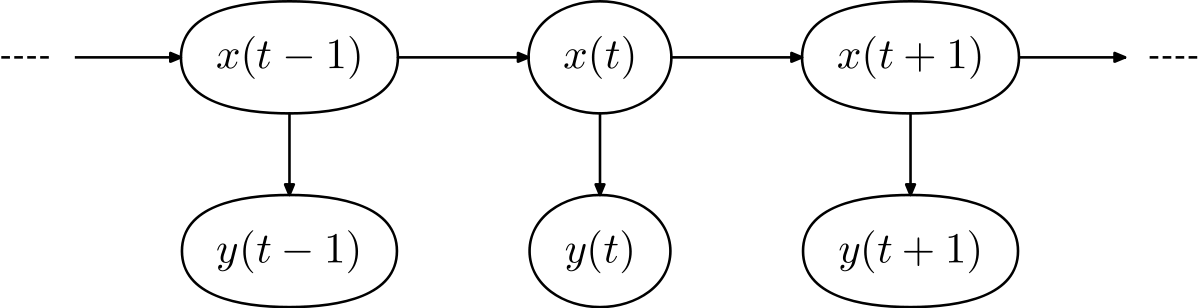
\includegraphics[width=.85\textwidth]{vreme.png}
  \caption{Ток времена код скривених Марковљевих модела \cite{vreme}}
  \label{fig:vreme}
\end{figure}

Сваки \textit{HMM}, наиме, моделује један Марковљев процес, што је поменуто при дефиницији. Последица је да тренутно стање зависи искључиво од претходног на путу и ниједног другог -- мапа $a$ моделује $p_{t-1} \mapsto p_t$, у ознакама са слике $x(t-1) \mapsto x(t)$. Исто тако, опсервација зависи искључиво од текућег стања -- мапа  $b$ моделује $p_t \mapsto o_t$, у ознакама са слике $x(t) \mapsto y(t)$. Стога се \textit{HMM} понекад дефинише и нешто другачије, као уређени пар $\{X, Y\}$, где је $X$ систем који се моделује, а $Y$ процес чије понашање директно зависи од $X$.

Прецизније, $X$ је Марковљев процес са неопсервабилним ("скривеним") стањима ($x$ из дефиниције), а циљ модела је да се нешто о том процесу сазна на основу опажања ($y$ из дефиниције) процеса $Y$, чије је понашање видљиво. Притом, условна расподела $Y$ (на слици конкретна вредност $y(t)$, а у низу опсервација приказ $o_t$) у неком временском тренутку $t$ (индекс низа) зависи искључиво од стања $X$ у том истом тренутку (на слици конкретна вредност $x(t)$, а на скривеном путу стање $p_t$). Приметно је да је ова дефиниција у суштини једнака претходно изложеним, с тим што је математички напреднија -- углавном је теже разумети торку апстрактних статистичких процеса него једноставних структура попут скупова, низова, матрица и мапа. На конкретном примеру непоштене коцкарнице, $X$ је процес одабира (замене) новчића, а $Y$ процес бацања новчића, односно добијања исхода тог бацања.

Свеукупно, описано временско својство оправдава употребу Витербијевог графа, чији је пример за проблем непоштене коцкарнице дат на слици \ref{fig:kockvit}. Граф се састоји из мреже (матрице) чворова чија основа има $n$ редова и $k$ колона. Свака колона састоји се од низа чворова који представљају сва скривена стања у тренутку $t$. Из сваког чвора у колони $t-1$ усмерена је по једна грана у сваки чвор из колоне $t$, на основу чињенице да се из сваког стања у тренутку $t-1$ може прећи у било које стање у тренутку $t$. Поред ове основе, мрежа има и два посебна чвора -- извор (експлицитно почетно стање) и понор (експлицитно завршно стање). Замисао овакве мреже је да истовремено моделује све скривене путеве дужине $k$ кроз \textit{HMM} са $n$ скривених стања.

\begin{figure}[H]
  \centering
  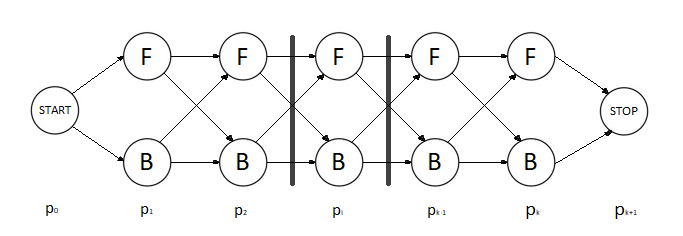
\includegraphics[width=\textwidth]{kock_graf.png}
  \caption{Витербијев граф непоштене коцкарнице}
  \label{fig:kockvit}
\end{figure}

Стварно, различитих путева од извора до понора има тачно $n^k$, и сваки одговара једном скривеном путу у \textit{HMM}. Остаје још питање како отежати гране Витербијевог графа, након чега се он може искористити за проблем максимизације кумулативне тежине у понору. То је заправо основни проблем над сваким Менхетн графом, који се може решити алгортмима динамичког програмирања, који обилазе чворове графа по тополошком редоследу.

За стицање интуиције у вези са моћи Витербијевог графа, корисно је увести проблем \ref{prob:maxput}. Задатак је пронаћи највероватнији скривени пут дужине $k$.

\begin{problem}[H]
  \SetAlgoLined
  \textit{Израчунати највероватнији скривени пут $p$ кроз \textit{HMM}.}\\
  \textbf{Улаз}: дужина $k$ скривеног пута кроз \textit{HMM}$\{a, b, \pi\}$.\\
  \textbf{Излаз}: највероватнији скривени пут $p_{opt} = p_1...p_k$.
  \caption{Највероватнији скривени пут}
  \label{prob:maxput}
\end{problem}

Наивно решење проблема своди се на већ разматрану исцрпну претрагу простора скривених путева, којих је $n^k$. Вероватноћа сваког пута рачуна се у $O(k)$ корака, па је временска сложеност експоненцијална $O(n^k k)$. Ипак, могуће је искористити Витербијев граф како би се постигло знатно побољшање.

Нека је мрежа чворова представљена мапом $s$, таквом да $s_{x_i, t}$ складишти неки податак о чвору (стању) $x_i$ у тренутку $t$. Оваква структура погодна је за свођење полазног проблема на проблем динамичког програмирања. Како је крајњи циљ максимизација вероватноће пута, нека $s_{x_i, t}$ заправо складишти вероватноћу оптималног пута дужине $t$ који се завршава у стању $x_i$. Очигледно, за путеве јединичне дужине, односно у тренутку $t=1$, важи: $$s_{x_i, 1} = P\{x_i\} = \pi_{x_i} = a_{\pi, x_i}.$$

Испоставља се да се и остале тежине могу узети из мапе прелаза, што важи због темпоралног својства Марковљевих процеса. Како свако стање зависи искључиво од првог претходног, тако се и вероватноћа нејединичног пута максимизује тако што се размотре сва могућа претходна стања, односно за једно стање краћи путеви. Тако важи следећа рекурентна формула: $$s_{x_i, t} = \max_j \{s_{x_j, t-1} \cdot a_{x_j, x_i}\},$$ $$P\{p_{opt}\} = \max_p P\{p\} = \max_j \{s_{x_j, k}\}.$$ Наравно, проблеми са рачуном се решавају логаритамском трансформацијом: $$s_{\log, x_i, 1} = P_{\log}\{x_i\} = \pi_{\log, x_i} = a_{\log, \pi, x_i},$$ $$s_{\log, x_i, t} = \max_j \{s_{\log, x_j, t-1} + a_{\log, x_j, x_i}\},$$ $$P_{\log}\{p_{opt}\} = \max_p P_{\log}\{p\} = \max_j \{s_{\log, x_j, k}\}.$$ Ова верзија је боља и због тога што су Менхетн алгоритми адитивни по природи, односно засновани су на сабирању, а не множењу вредности. Слика \ref{fig:tribac} приказује како Витербијев граф моделује три бацања у непоштеном казину.

\begin{figure}[H]
  \centering
  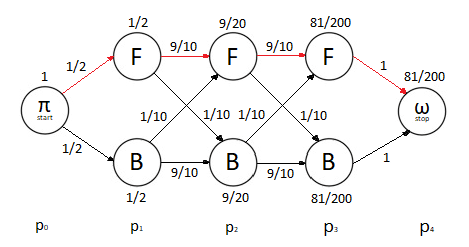
\includegraphics[width=.9\textwidth]{tri_bacanja.png}
  \caption{Максимизација $P\{p\}$ са три бацања}
  \label{fig:tribac}
\end{figure}

Општи облик ове рекурентне релације заправо је заснован на тежинама грана $\tau$, где мапа облика $\tau_{x_i, x_j, t}$ означава тежину гране из чвора $x_i$ ка $x_j$ у тренутку $t$, укључујући експлицитни почетни извор $\pi$ и завршни понор $\omega$. Оне су у конкретном случају биле логаритми вероватноћа преласка или саме вероватноће, као на слици, у ком случају се множи уместо сабира: $$s_{x_i, 1} = \tau_{\pi, x_i}, s_{x_i, t} = \max_j \{s_{x_j, t-1} + \tau_{x_j, x_i, t}\},$$ $$P_{opt} = \max_j \{s_{x_j, k} + \tau_{x_j, \omega}\}.$$

Како је моделовано $P\{p\}$, тако се може моделовати и $P\{p, o\}$ за фиксирано $o$. У првом случају, важило је $\tau_{x_i, x_j, t} = \tau_{x_i, x_j} = a_{x_i, x_j}$, док је у другом нешто сложеније $\tau_{x_i, x_j, t} = a_{x_i, x_j} \cdot b_{x_j, o_t}$, дакле вероватноћа догађаја да \textit{HMM} пређе из стања $x_i$ у стање $x_j$, након чега емитује симбол $o_t$. Формуле су сада: $$s_{x_i, 1} = \pi_{x_i} \cdot b_{x_i, o_1} = a_{\pi, x_i} \cdot b_{x_i, o_1},$$ $$s_{x_i, t} = \max_j \{s_{x_j, t-1} \cdot a_{x_j, x_i} \cdot b_{x_i, o_t}\},$$ $$P\{p_{opt}, o\} = \max_p P\{p, o\} = \max_j \{s_{x_j, k}\}.$$ Логаритамске верзије се изводе аналогно.

Када се говори о проблему максимизације, могуће је моделовати и $P\{o | p\}$, с тим што за то није неопходан Витербијев граф. Поставка \ref{prob:maxpops} је у наставку.

\begin{problem}[H]
  \SetAlgoLined
  \textit{Израчунати највероватнији низ емисија на путу $p$ кроз \textit{HMM}.}\\
  \textbf{Улаз}: скривени пут $p = p_1...p_k$ кроз \textit{HMM}$\{a, b, \pi\}$.\\
  \textbf{Излаз}: највероватнија опажања $o_{opt} = o_1...o_k$ на путу $p$.
  \caption{Највероватније опсервације на путу}
  \label{prob:maxpops}
\end{problem}

Формула максималне вероватноће је једноставна, по свакој опсервацији: $$P\{o_{opt} | p\} = \prod_{i=1}^k \max_j b_{p_i, y_j}.$$

Претходно изложени систем рада са \textit{HMM}, заснован на Витербијевом графу и динамичком програмирању назива се Витербијев алгоритам \cite{ba10c}, посебно када се примењује на декодирање -- проблем \ref{prob:dekod}. Изведеним рекурентним формулама још само треба додати систем путоказа, како би поред вероватноће оптималног пута могао бити добијен (реконструисан) и сам пут.

Важна предност Витербијевог алгоритма је његова сложеност. Основна мрежа графа има $nk$ чворова и $n^2 (k-1)$ грана (из свих $n$ стања ка свим $n$ стањима у $k-1$ временском прелазу), чему се додају још два додатна чвора и $2n$ грана повезаних са тим чворовима. Израчунавање иде по чворовима, користећи гране, тако да је укупна временска и просторна сложеност $O(n^2 k)$ уколико би се користио експлицитни граф. Ово је временски знатно боље од наивних $O(n^k k)$, али је просторно захтевније, јер наивни приступ захтева само $O(k)$ помоћног простора. Ради се о уобичајеном компромису између времена и простора, када алгоритам за бржи рад захтева више меморије.

У многим случајевима је, међутим, граф довољно само замислити, а у раду користити искључиво мапу $s$ и путоказе, а не и тежине $\tau$, што за собом повлачи нешто бољу просторну сложеност $O(nk)$. Ово важи код декодирања, јер су тежине (гране) већ похрањене у мапама $a$ и $b$. Други начин побољшања је ако се $\tau$ представи као функција уместо мапа, што је такође могуће код проблема декодирања, јер тежине не зависе од временског тренутка. Додатно, уколико је довољно добити само максималну вероватноћу, а не и сам пут, не треба чувати путоказе, а мапу $s$ могуће је свести на два низа који се наизменично попуњавају, чиме се просторна сложеност своди на $O(n)$.

У практичним применама је могуће постићи још бољу сложеност. Наиме, многи \textit{HMM} имају забрањене прелазе између неких стања. Таква ситуација веома је честа, а приказана је још на уводној слици \ref{fig:hmm}. Могуће је без проблема уклонити гране Витербијевог графа које одговарају таквим прелазима, што знатно смањује време извршавања алгоритма. Посебно занимљиви могу бити недозвољени прелази који укључују извор и понор. На тај начин се може онемогућити да неко стање буде полазно или завршно, што често има биолошки смисао, о чему ће бити речи на примеру профилних модела протеина.

% Finding the Most Likely Outcome of an HMM
\section{Алгоритам "напред"}
Сваки \textit{HMM}, подсећања ради, може се схватити као уређени пар два процеса -- скривеног Марковљевог који се очитава скривеним путем $p$ и опсервабилног зависног који се очитава низом емисија $o$. Цела идеја \textit{HMM} јесте детаљно статистички потковано моделовање тих процеса и њиховог односа.

Досад је било речи о појединачној расподели $P\{p\}$, условној $P\{o | p\}$ и заједничкој $P\{p, o\}$. Како је код последњег подразумевано да је позната ниска $o$, тиме је заправо моделована и условна расподела $P\{p | o\}$. Могуће је моделовати и појединачну расподелу $P\{o\}$, која је једина преостала како би модел био комплетиран. Основни задатак из овог домена дат је кроз проблем \ref{prob:ops}. Потребно је израчунати вероватноћу да \textit{HMM} емитује неку ниску дужине $k$.

\begin{problem}[H]
  \SetAlgoLined
  \textit{Израчунати вероватноћу приказа $o$ у \textit{HMM}.}\\
  \textbf{Улаз}: низ опажања $o = o_1...o_k$ у \textit{HMM}$\{a, b, \pi\}$.\\
  \textbf{Излаз}: вероватноћа улазног низа опажања $P\{o\}$.
  \caption{Вероватноћа опсервација \cite{ba10d}}
  \label{prob:ops}
\end{problem}

Још једном, наивни приступ састоји се од генерисања свих $n^k$ путева и сумирања вероватноћа на њима, према раније изложеној маргинализацији $P\{o\} = \sum_p P\{p, o\}$. Занимљиво је, међутим, приметити да је ова маргинализација врло слична садржају мапе $s$ код Витербијевог алгоритма, која у понору израчунава $P\{p_{opt}, o\} = \max_p P\{p, o\}$. Једина разлика је у примењеном оператору -- да ли је сума или максимум. Ово није случајно, јер је идеја обе формуле обилазак свих скривених путева кроз \textit{HMM} истовремено.

Свеукупно, сасвим је оправдано увести нову мапу $f$ (од енгл. \textit{forward} -- напред), надахнуту претходном $s$ (од енгл. \textit{score} -- скор), такву да елемент $f_{x_i, t}$ складишти вероватноћу префикса опажања дужине $t$ (подниз $o_1...o_t$), насталог на скривеном путу који завршава стањем $x_i$. Одатле су формуле: $$f_{x_i, 1} = \pi_{x_i} \cdot b_{x_i, o_1} = a_{\pi, x_i} \cdot b_{x_i, o_1},$$ $$f_{x_i, t} = \sum_j f_{x_j, t-1} \cdot a_{x_j, x_i} \cdot b_{x_i, o_t},$$ $$P\{o\} = \sum_j f_{x_j, k}.$$ Као и досад, логаритамске верзије производе мењају збировима. Овога пута има и један додатак: сума се мења посебним оператором -- $\operatorname{logsumexp}_j f(j)$. Он моделује сабирање у логаритамском домену, тј. апроксимира $\log \sum_j e^{f(j)}$.

У наставку, ваља поменути и сродан проблем одређивања највероватнијег исхода, односно $o_{opt} = \operatorname{argmax}_o P\{o\}$. Формулација је дата проблемом \ref{prob:maxops}.

\begin{problem}[H]
  \SetAlgoLined
  \textit{Израчунати највероватнији низ емисија у \textit{HMM}.}\\
  \textbf{Улаз}: дужина $k$ пута кроз \textit{HMM}$\{a, b, \pi\}$.\\
  \textbf{Излаз}: највероватнија опажања $o_{opt} = o_1...o_k$.
  \caption{Највероватније опсервације}
  \label{prob:maxops}
\end{problem}

И овде је наивно решење сувише неефикасно. Штавише, лошије је сложености од досадашњих $O(n^k k)$, јер је сада потребно генерисати и сваки могући низ опсервација. Сложеност исцрпне претраге стога је $O(n^k m^k k)$. Нешто боља сложеност добија се ако се не генеришу сви путеви, јер се свако од укупно $m^k$ опажања може оценити већ изложеним алгоритмом "напред". Тада је свеукупна сложеност $O(n^2 m^k k)$. Напредно решење може се конструисати помоћу тродимензионе верзије Витербијевог графа \cite{compeau2015}, где нову димензију чине све могуће опсервације по моделу. Сада је идеја применом оба оператора заредом успешно максимизовати суму $\max_o \sum_p P\{p, o\} = P\{o_{opt}\}$.

Алтернативни поглед на ствари подразумева остајање у дводимензионом простору -- замисао је да из сваког од $n$ стања (такође и почетног $\pi$) ка свим $n$ стањима у $k-1$ временском прелазу иде по $m$ грана, по једна за сваку могућу опсервацију. Тиме гране Витербијевог (мулти)графа више не моделују само прелазе из једног стања у друго, већ успут и емисије. Тежине се одабирају тако да осликавају вероватноћу промене стања, а затим емитовања симбола представљеног граном. Сваки пут од извора до понора сада није само скривени пут $p$, већ пут $p$ (чворови) са придруженим опажањима $o$ (гране). Максимални збир добија се максимизирањем сума између нивоа. Сложеност је у том случају $O(n^2 m k)$, а формуле (логаритамске су аналогне): $$f_{x_i, 1} = \max_k \{\pi_{x_i} \cdot b_{x_i, y_k}\} = \max_k \{a_{\pi, x_i} \cdot b_{x_i, y_k}\},$$ $$f_{x_i, t} = \max_k \sum_j f_{x_j, t-1} \cdot a_{x_j, x_i} \cdot b_{x_i, y_k},$$ $$P\{o_{opt}\} = \max_o P\{o\} = \sum_j f_{x_j, k}.$$

Заменом суме максимумом у претходним формулама, добија се највероватнији пар скривеног пута дужине $k$ и на њему емитоване ниске симбола. То је решење проблема \ref{prob:maxpo}, сличног досад разматранима.

\begin{problem}[H]
  \SetAlgoLined
  \textit{Израчунати највероватнији пут и опажања у \textit{HMM}.}\\
  \textbf{Улаз}: дужина $k$ пута кроз \textit{HMM}$\{a, b, \pi\}$.\\
  \textbf{Излаз}: највероватнија комбинација пута $p$ и опажања $o$.
  \caption{Највероватнији скривени пут и опсервације}
  \label{prob:maxpo}
\end{problem}

То је $\max P\{p, o\}$, што је исплативије од $n^k m^k$ или $n^2 m^k$ наивних покушаја (и овде се логаритамске верзије изводе аналогно, па се не наводе): $$f_{x_i, 1} = \max_k \{\pi_{x_i} \cdot b_{x_i, y_k}\} = \max_k \{a_{\pi, x_i} \cdot b_{x_i, y_k}\},$$ $$f_{x_i, t} = \max_{j, k} \{f_{x_j, t-1} \cdot a_{x_j, x_i} \cdot b_{x_i, y_k}\},$$ $$\max P\{p, o\} = \max_j \{f_{x_j, k}\}.$$

Комплетности ради, могу се формално представити и проблеми \ref{prob:putpri} и \ref{prob:maxputpri}, којима се експлицитно израчунава $P\{p | o\}$ и $\max_p P\{p | o\}$ за познато $o$.

\begin{problem}[H]
  \SetAlgoLined
  \textit{Израчунати вероватноћу пута $p$ кроз \textit{HMM} ако је опажено $o$.}\\
  \textbf{Улаз}: ниска $o = o_1...o_k$ коју је емитовао \textit{HMM}$\{a, b, \pi\}$ и скривени пут $p = p_1...p_k$ кроз који је прошао.\\
  \textbf{Излаз}: условна вероватноћа пута при приказу $P\{p | o\}$.
  \caption{Вероватноћа пута при исходу}
  \label{prob:putpri}
\end{problem}

Сама вероватноћа пута ако је опажена нека секвенца емисија може се израчунати преко формуле условне вероватноће. Решење је, дакле: $$P\{p | o\} = \frac{P\{p, o\}}{P\{o\}}.$$ Главнина оваквог приступа је израчунавање вероватноће исхода, тако да је сложеност $O(n^2 k)$. Наивни приступ би, као и досад, узео $O(n^k k)$ времена.

\begin{problem}[H]
  \SetAlgoLined
  \textit{Израчунати највероватнији пут $p$ кроз \textit{HMM} ако је опажено $o$.}\\
  \textbf{Улаз}: ниска $o = o_1...o_k$ коју је емитовао \textit{HMM}$\{a, b, \pi\}$.\\
  \textbf{Излаз}: највероватнију пут $p_{opt} = p_1...p_k$ ако је опажено $o$.
  \caption{Највероватнији пут при исходу}
  \label{prob:maxputpri}
\end{problem}

Максимизација је још једноставнија, када се примети раније поменуто $\operatorname*{argmax}_p P\{p, o\} = \operatorname*{argmax}_p P\{p | o\}$ за познато $o$. Ово значи да је довољно искористити решење проблема \ref{prob:dekod}, уз прикладно скалирање вероватноће.

Сада је познато како Витербијевим графом моделовати и максимизовати сваку од критичних вероватноћа $P\{p\}$, $P\{o\}$, $P\{p, o\}$, $P\{p | o\}$ и $P\{o | p\}$, чиме је модел комплетиран, барем што се тиче његове описне стране (остаје учење). Досадашња постигнућа модела сумирана су табелом \ref{tab:hmm}, која следи.

\begin{table}[h!]
  \centering
  \caption{Могућности скривених Марковљевих модела}
  \begin{tabular}{| c c c c | c c |} \hline
  \multicolumn{4}{| c |}{Проблем -- алгоритам} & \multicolumn{2}{ c |}{Сложеност} \\
  Број & Улаз & Циљ & Вредност & Наивни & Напредни \\ \hline
  \ref{prob:dekod}      & $o_k$             & $\operatorname*{(arg)max}_p$ & $P\{p, o\}$  & $O(n^k k)$  & $O(n^2 k)$  \\
  \ref{prob:putishod}  & $p_k$, $o_k$  & --                                               & $P\{p, o\}$  & $O(k)$         & -- \\
  \ref{prob:put}          & $p_k$             & --                                               & $P\{p\}$      & $O(k)$         & -- \\
  \ref{prob:ishod}       & $p_k$, $o_k$  & --                                               & $P\{o | p\}$ & $O(k)$         & -- \\
  \ref{prob:maxput}    & $k$                & $\operatorname*{(arg)max}_p$ & $P\{p\}$       & $O(n^k k)$  & $O(n^2 k)$ \\
  \ref{prob:maxpops}  & $p_k$            & $\operatorname*{(arg)max}_o$ & $P\{o | p\}$  & $O(m^k k)$ & $O(m k)$ \\
  \ref{prob:ops}          & $o_k$            & --                                               & $P\{o\}$       & $O(n^k k)$  & $O(n^2 k)$ \\
  \ref{prob:maxops}    & $k$               & $\operatorname*{(arg)max}_o$  & $P\{o\}$       & \dvareda{$O(n^k m^k k)$ \\ $O(n^2 m^k k)$} & $O(n^2 m k)$ \\
  \ref{prob:maxpo}      & $k$               & $\operatorname*{(arg)max}_{p, o} $ & $P\{p, o\}$ & \dvareda{$O(n^k m^k k)$ \\ $O(n^2 m^k k)$} & $O(n^2 m k)$ \\
  \ref{prob:putpri}       & $p_k$, $o_k$  & --                                              & $P\{p | o\}$ & $O(n^k k)$ & $O(n^2 k)$ \\
  \ref{prob:maxputpri} & $o_k$            & $\operatorname*{(arg)max}_p$ & $P\{p | o\}$ & \dvareda{$O(n^{2k} k)$ \\ $O(n^k k)$} & $O(n^2 k)$ \\ \hline
  \end{tabular}
  \label{tab:hmm}
\end{table}

% ------------------------------------------------------------------------------
\chapter{Биолошки значај}
% ------------------------------------------------------------------------------
Након дефинисања скривених Марковљевих модела, описа њихове примене и алгоритама који дају одговоре на важна питања у вези са моделованим проблемом, у овој глави је непосредно описан биолошки значај \textit{HMM}, односно њихова примена у досад изложеним биоинформатичким проблемима. Конкретно, глава која следи бави се потрагом за генима, односно откривањем \textit{CG} острва помоћу \textit{HMM}, као и употребом профилних \textit{HMM} за решавање проблема попут откривања фенотипа ХИВ-а.

\section{Гени -- два стања}
У уводном делу, посвећеном мотивацији, дискутовано је о проналажењу места на којима се гени налазе, односно где њихово преписивање (транскрипција) започиње. Објашњено је зашто је удео динуклеотида \textit{CG} мали у некодирајућим регионима ДНК, а нешто већи у кодирајућим, те како има смисла ту чињеницу искористити за откривање такозваних \textit{CG} острва (\textit{CpG} места), што су региони богати генима. Имплементиран је и наиван приступ решавању овог проблема, заснован на клизећем прозору, али су уз њега остале неразјашњене важне недоумице: како одредити добру величину прозора, као и шта тачно радити када преклапајући прозори нуде различиту класификацију подниза.

Сада је циљ доћи до прецизног, једнозначног и статистички поткованог решења употребом одговарајућег скривеног Марковљевог модела. Замисао је у суштини једноставна -- улазни низ нуклеотида посматра се као секвенца опажања коју треба декодирати. Другим речима, за сваки карактер ниске са улаза потребно је одредити да ли је вероватније настао као емисија \textit{CG} острва или не, што је заправо позадински скривени процес. Стога важи следеће:
\begin{itemize}
  \item скривена стања $x = \{+, -\}$ -- јесте \textit{CG} острво или није,
  \item опсервације $y = \{A, C, G, T\}$ -- азбука ДНК нуклеотида.
\end{itemize}

Скупови скривених стања и могућих опажања се, дакле, лако одређују, па чак и веома личе на разматрани проблем непоштене коцкарнице. Наиме, такође су присутна два стања, мада опсервација има нешто више. Свеукупно, проблем се може апстраховати неком врстом коцкарнице, у којој крупије мења две различито отежане четворостране коцкице. Уопштени дијаграм (без вероватноћа) оваквог модела приказан је на слици \ref{fig:cg_graf}.

\begin{figure}[H]
  \centering
  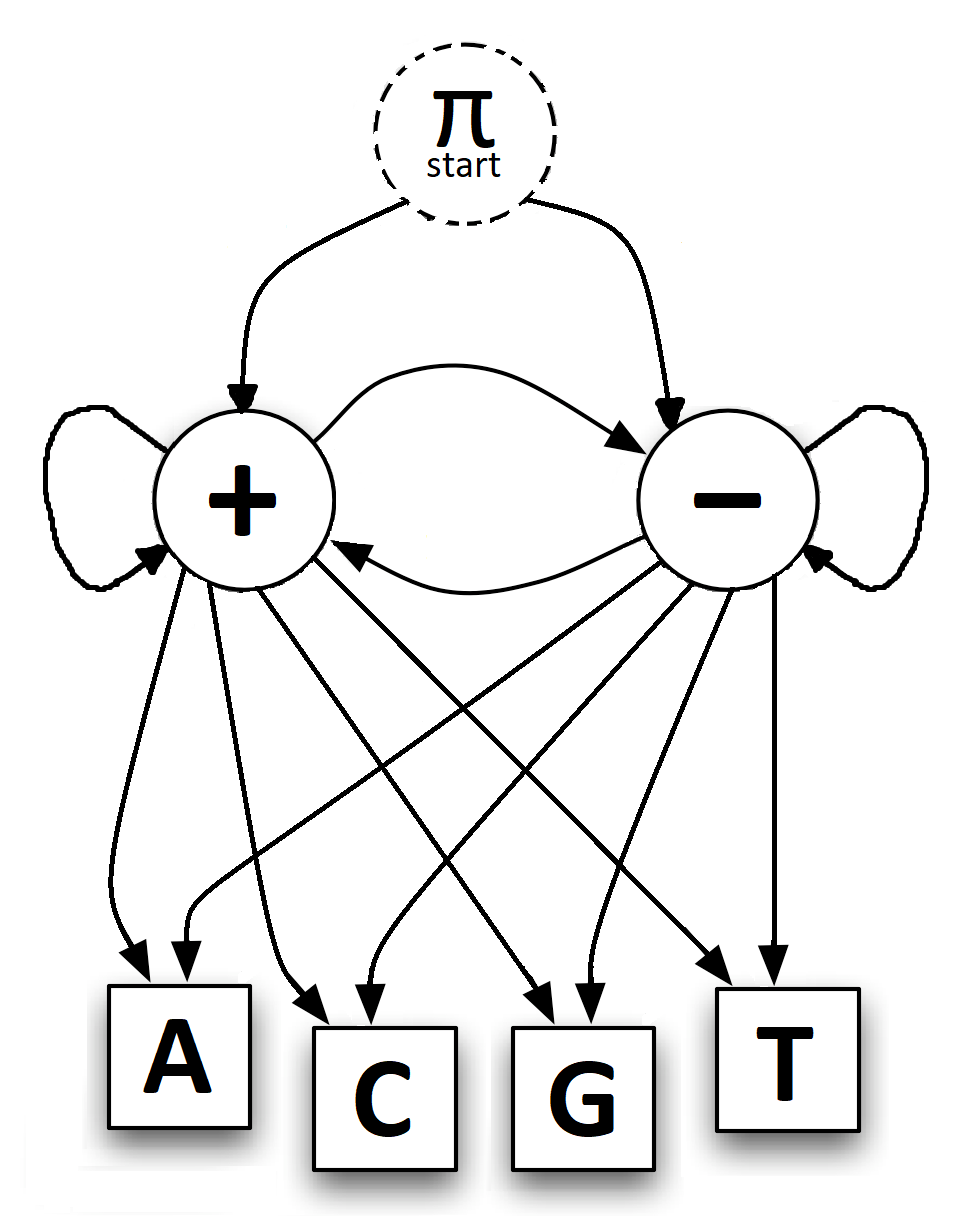
\includegraphics[width=.5\textwidth]{cg_graf.png}
  \caption{Скривени модел \textit{CG} острва са два стања}
  \label{fig:cg_graf}
\end{figure}

Остаје још одредити све битне вероватноће. За овај део задатка погодује применити прави биоинформатички приступ. Подсећања ради, биоинформатика је у уводу дефинисана као интердисциплинарна област која се бави применом рачунарских технологија у области биологије и сродних наука, са нагласком на разумевању биолошких података. Наведено је да статистички (математички) апаратат служи за рад са подацима, рачунарске технологије тај апарат чине употребљивијим, док биологија даје потребно доменско знање (разумевање) за рад са биолошким и сродним подацима. Управо је то овде и примењено -- статистика (математика) дефинише појам \textit{HMM}, а рачунарске технологије (конкретно \textit{Python} и \textit{Jupyter}) ефикасно га имплементирају.

Потребно је још консултовати се са биологијом, а овде заправо и генетиком, како би се адекватно одредили параметри модела. За почетак, треба приметити да се може добити фактички било какав исечак ДНК секвенце. Другим речима, не постоји гаранција да ће почетни регион бити кодирајући или не, тако да је најсигурније равномерно расподелити почетна стања:
\begin{itemize}
  \item полазне вероватноће $\pi = \begin{pNiceMatrix}[first-col] + & 0,5 \\ - & 0,5 \end{pNiceMatrix}$ -- равномеран почетак.
\end{itemize}

Даље, питање је колико често долази до промене стања. Одговор је да се то дешава веома ретко, с тим што мањи део секвенце представља \textit{CG} острво, тако да је нешто већа шанса да дође до напуштања \textit{CG} острва, него уласка у њега. Свеукупно, могла би се одабрати мапа прелаза попут следеће:
\begin{itemize}
  \item прелази $a = \begin{pNiceMatrix}[first-row,first-col] & + & - \\ + & 0,98 & 0,02 \\ - & 0,01 & 0,99 \end{pNiceMatrix}$ -- мала могућност промене.
\end{itemize}

За крај, остаје најтеже питање: како моделовати вероватноће опажања. Постоје разни приступи, а један од њих заснован је на емпиријским подацима. Примера ради, уколико се трага за генима у људском \textit{X} хромозому, могу се апроксимирати вероватноће нуклеотида на основу вероватноћа динуклеотида из таблице \ref{tab:cg}. Резултат тога је следећа мапа вероватноћа опсервација:
\begin{itemize}
  \item емисије $b = \begin{pNiceMatrix}[first-row,first-col] & A & C & G & T \\ + & 0,222 & 0,2555 & 0,299 & 0,2235 \\ - & 0,274 & 0,227 & 0,2295 & 0,2695 \end{pNiceMatrix}$ -- емпиријски.
\end{itemize}
Очекивано, нешто је већи удео цитозина и гуанина у кодирајућим регионима. Важи и супротно -- нешто је већи удео аденина и тимина у некодирајућим регионима \textit{X} хромозома, што је такође очекивана повезана појава.

Овакав модел, међутим, није успешан јер су вероватноће тако постављене да није могуће препознати мала \textit{CG} острва. Приликом декодирања, закључак ће за сваку малу секвенцу бити да је највероватније цела (не)кодирајућа, из једноставног разлога што је свака промена стања веома скупа, а удео нуклеотида није толико различит. Стога се може добити побољшање уколико се вероватноће прелаза мало приближе, а емисија мало више удаље.

То се може учинити тако што се, за почетак, вероватноће промене стања поставе на нешто већу једну десетину. Ако је \textit{HMM} у некодирајућем стању, може се претпоставити да је расподела нуклеотида равномерна -- сваки се емитује са могућношћу једне четвртине. У супротном, сматра се да се цитозин и гуанин приказују четири пута чешће. Резултујуће вероватноће сада су:
\begin{itemize}
  \item прелази $a = \begin{pNiceMatrix}[first-row,first-col] & + & - \\ + & 0,9 & 0,1 \\ - & 0,1 & 0,9 \end{pNiceMatrix}$ -- већа могућност промене,
  \item емисије $b = \begin{pNiceMatrix}[first-row,first-col] & A & C & G & T \\ + & 0,1 & 0,4 & 0,4 & 0,1 \\ - & 0,25 & 0,25 & 0,25 & 0,25 \end{pNiceMatrix}$ -- поправљено.
\end{itemize}

Нажалост, ни овај модел није бољи. Параметри су, иначе, преузети са примера употребе библиотеке \textit{pomegranate} \cite{schreiber2021}, која је детаљније описана у практичном делу електронске лекције. Поред ње, у додатку лекције представљен је још један познати модул језика \textit{Python} за рад са скривеним Марковљевим моделима -- \textit{hmmlearn} \cite{lee2021}. Оба су употребљена за потрагу за генима.

Трећа идеја за добијање бољег резултата могло би бити додатно повећавање вероватноће промене стања. Мала повећања не би променила резултат, док би већа изврнула смисао \textit{CpG} места -- острвом би се прогласио сваки цитозин и гуанин. Ова чињеница није необична и у складу је са тим да оваква употреба \textit{HMM} спада под домен ненадгледаног учења, где модел по самосталној процени групише поднизове улазне секвенце. То значи да се лако могу добити неочекивани или незадовољавајући резултати, попут једноставне поделе према текућем карактеру.

Следећа идеја настоји да проблем превазиђе тако што укључује већи број опажања. Наиме, могуће је ДНК секвенцу схватити као низ динуклеотида уместо самих нуклеотида, као код прозорског приступа. Сада важи следеће:
\begin{itemize}
  \item опсервације $y = \{A, C, G, T\} \times \{A, C, G, T\}$ -- азбука динуклеотида.
\end{itemize}
Може се изменити и мапа прелаза, док се мапа емисија узима према табели \ref{tab:cg}, која управо непосредно приказује вероватноће динуклеотида. Овај приступ даје засад најбоље резултате, који се могу видети у коду лекције.

Важна досад занемарена чињеница јесте да су \textit{HMM} генеративни модели. Не само што служе за опис појава које моделују, већ могу и да их опонашају. Досад је размотрено како се могу добити скривени путеви или опажања који максимизују неку вероватноћу. Испоставља се да се још једноставније добијају произвољан скривени пут и исход на њему. Пут жељене дужине генерише се на основу мапе преласка, а исход на путу помоћу мапе емисија. Претходни модел за откривање гена тако се може искористити за генерисање вештачке ДНК секвенце, која задовољава статистички опис ДНК. Она, наиме, у појединим деловима садржи \textit{CG} острва и тиме се чини природнијом од случајно генерисане ниске над азбуком нуклеотида, што је додатна корист од \textit{HMM}.

\section{Гени -- више стања}
Како је већ напоменуто, сви досадашњи модели су по структури подсећали на непоштени казино -- имали су два стања која се ретко мењају и углавном четири опсервације, мада је најбољи резултат добијен при последњем покушају, са чак шеснаест различитих динуклеотидних емисија. Алтернативна идеја увођењу већег броја исхода јесте увођење већег броја стања, што се најчешће реализује кроз два приступа, који су представљени у наставку.

\begin{figure}[H]
  \centering
  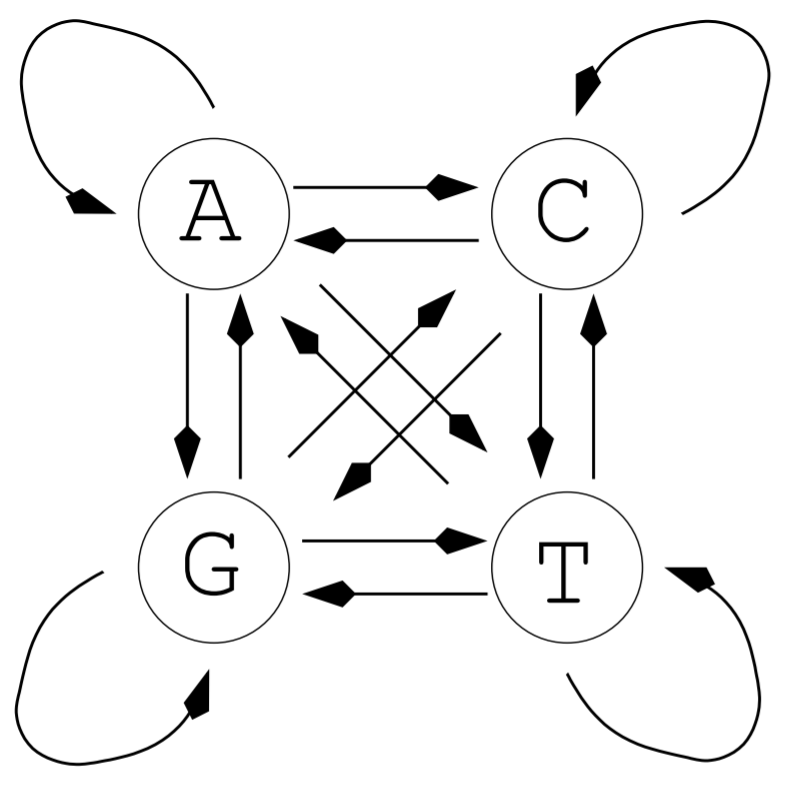
\includegraphics[width=.5\textwidth]{cg_lanac.png}
  \caption{Марковљев ланац за моделовање ДНК секвенце \cite{huson2020}}
  \label{fig:cg_lanac}
\end{figure}

Полазна идеја првог приступа \cite{holmes2012, huson2020, kellis2021, shamir2009} јесте да се \textit{CG} острва и региони ван њих могу моделовати као два одвојена Марковљева ланца (подсећања ради, они су \textit{HMM} без емисија, а скраћено се називају \textit{MC}). Стања ланаца су јавна (то јест, нису скривена), пошто верно прате ДНК секвенцу коју моделују, и одговарају азбуци нуклеотида, па се могу представити сликом \ref{fig:cg_lanac}.

Одговарајуће матрице прелаза могу се одредити емпиријским путем, дакле обрадом секвенци за које је познато јесу ли \textit{CG} острва или не. Уобичајено се узимају вредности из табеле \ref{tab:cg_lanac}, које су унапред израчунате.

\begin{table}[h!]
  \centering
  \caption{\dvareda{Вероватноћа прелаза између нуклеотида једне секвенце\\-- лево у регионима \textit{CG} острва, а десно ван њих \cite{shamir2009}}}
  \begin{tabular}{| c | c c c c | c c c c |} \hline
   & A & C & G & T & A & C & G & T \\ \hline
  A & 0,180 & 0,274 & 0,426 & 0,120 & 0,300 & 0,205 & 0,285 & 0,210 \\
  C & 0,171 & 0,367 & 0,274 & 0,188 & 0,322 & 0,298 & 0,078 & 0,302 \\
  G & 0,161 & 0,339 & 0,375 & 0,125 & 0,248 & 0,246 & 0,298 & 0,208 \\
  T & 0,079 & 0,355 & 0,384 & 0,182 & 0,177 & 0,239 & 0,292 & 0,292 \\ \hline
  \end{tabular}
  \label{tab:cg_lanac}
\end{table}

Аналогно прозорском приступу заснованом на динуклеотидном садржају секвенце и табели \ref{tab:cg}, могуће је помоћу \textit{MC} за сваки подниз одредити да ли је већа вероватноћа да јесте \textit{CG} острво или да није. Бројчана сагласност се за оба \textit{MC} може израчунати већ имплементираним алгоритмом за одређивање вероватноће пута кроз \textit{HMM}, као решење проблема \ref{prob:put}. Одабир припадности пада на ланац са већом вероватноћом. Резултати су једнаки као у првом покушају, а остају нерешени проблеми прозорског приступа: како одредити добру величину прозора и како разрешити сукобе настале преклапањем прозора.

\begin{figure}[H]
  \centering
  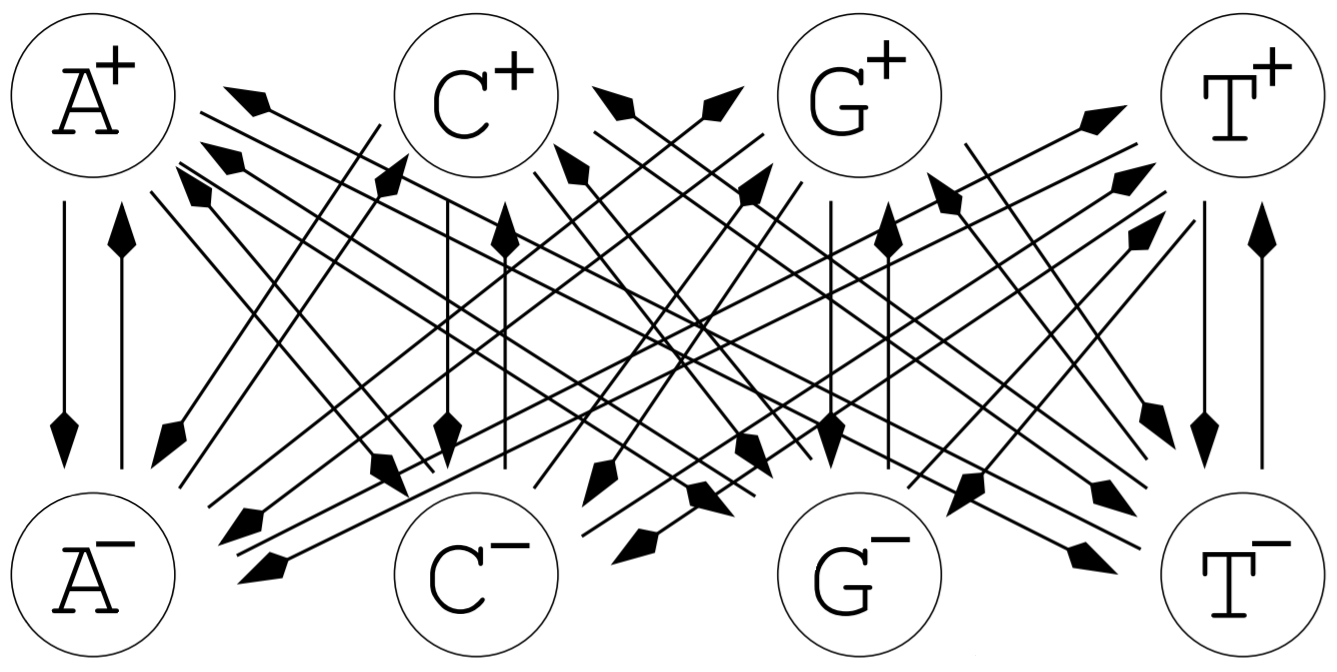
\includegraphics[width=.75\textwidth]{cg_lanci.png}
  \caption{Спојени ланци за моделовање \textit{CG} острва \cite{huson2020}}
  \label{fig:cg_lanci}
\end{figure}

Као решење, предлаже се спајање ова два ланца у један. Резултујући \textit{MC} дат је на слици \ref{fig:cg_lanci}. Он сада има осам стања, за сваки пар нуклеотида и припадности \textit{CG} острву. Једноставности ради, пошто укупно има $8^2 = 64$ прелаза, приказани су само нови, док се стари (слика \ref{fig:cg_lanac}) подразумевају.

Пре свега, неопходно је одредити нову, заједничку матрицу преласка. За то се треба подсетити већ поменутог доменског биолошког знања, према коме је мало вероватан прелазак из кодирајућег у некодирајуће стање (нпр. само 2 \%), а још мање вероватно обрнуто (нпр. тек 1 \%). Нове вероватноће могу се добити скалирањем старих, нпр. на начин представљен табелом \ref{tab:cg_hmm1}.

\begin{table}[h!]
  \centering
  \caption{Вероватноћа прелаза унутар \textit{CG} острва}
  \begin{tabular}{| c | c c c c |} \hline
   & $A^+$ & $C^+$ & $G^+$ & $T^+$ \\ \hline
  $A^+$ & 0,180p & 0,274p & 0,426p & 0,120p \\
  $C^+$ & 0,171p & 0,367p & 0,274p & 0,188p \\
  $G^+$ & 0,161p & 0,339p & 0,375p & 0,125p \\
  $T^+$ & 0,079p & 0,355p & 0,384p & 0,182p \\ \hhline{= | = = = =}
   & $A^-$ & $C^-$ & $G^-$ & $T^-$ \\ \hline
  $A^+$ & 0,180(1-p) & 0,274(1-p) & 0,426(1-p) & 0,120(1-p) \\
  $C^+$ & 0,171(1-p) & 0,367(1-p) & 0,274(1-p) & 0,188(1-p) \\
  $G^+$ & 0,161(1-p) & 0,339(1-p) & 0,375(1-p) & 0,125(1-p) \\
  $T^+$ & 0,079(1-p) & 0,355(1-p) & 0,384(1-p) & 0,182(1-p) \\ \hline
  \end{tabular}
  \label{tab:cg_hmm1}
\end{table}

Идеја је, дакле, расподелити вероватноће претходних прелаза унутар \textit{CG} острва типа $P\{N \mapsto M\}$ на две нове типа $P\{N^+ \mapsto M^+\} = p P\{N \mapsto M\}$ и $P\{N^+ \mapsto M^-\} = (1-p) P\{N \mapsto M\}$, где $p$ представља вероватноћу останка унутар острва, нпр. $p = 98 \%$. Аналогно томе, вероватноће претходних прелаза ван \textit{CG} острва типа $P\{N \mapsto M\}$ могу се расподелити на две нове типа $P\{N^- \mapsto M^-\} = q P\{N \mapsto M\}$ и $P\{N^- \mapsto M^+\} = (1-q) P\{N \mapsto M\}$, где $q$ представља вероватноћу останка ван острва, нпр. $q = 99 \%$. Алтернативна је равномерно расподелити вероватноће промене стања, као у табели \ref{tab:cg_hmm2}.

\begin{table}[h!]
  \centering
  \caption{Вероватноћа прелаза ван \textit{CG} острва}
  \begin{tabular}{| c | c c c c |} \hline
   & $A^-$ & $C^-$ & $G^-$ & $T^-$ \\ \hline
  $A^-$ & 0,300q & 0,205q & 0,285q & 0,210q \\
  $C^-$ & 0,322q & 0,298q & 0,078q & 0,302q \\
  $G^-$ & 0,248q & 0,246q & 0,298q & 0,208q \\
  $T^-$ & 0,177q & 0,239q & 0,292q & 0,292q \\ \hhline{= | = = = =}
   & $A^+$ & $C^+$ & $G^+$ & $T^+$ \\ \hline
  $A^-$ & (1-q)/4 & (1-q)/4 & (1-q)/4 & (1-q)/4 \\
  $C^-$ & (1-q)/4 & (1-q)/4 & (1-q)/4 & (1-q)/4 \\
  $G^-$ & (1-q)/4 & (1-q)/4 & (1-q)/4 & (1-q)/4 \\
  $T^-$ & (1-q)/4 & (1-q)/4 & (1-q)/4 & (1-q)/4 \\ \hline
  \end{tabular}
  \label{tab:cg_hmm2}
\end{table}

Сада се спојени Марковљев ланац може и мора надградити у скривени Марковљев модел. Наиме, два одвојена \textit{MC} била су смислена без унапређења, јер су имала само четири суштински јавна стања, која одговарају нуклеотидима из опажене секвенце. Нових осам стања је, међутим, по природи скривено, јер опажањем секвенце није познато у ком је модел стању, као у непоштеној коцкарници и другим моделима. Примера ради, већ за једночлани исход $G$ није јасно да ли је настао у стању $G^+$ или $G^-$. Ниска дужине $k$ може настати на $2^k$ различитих непознатих путева, који су стога скривени.

Већ је имплицирано да симбол $N$ може приказати само стање типа $N^+$ и $N^-$. Важи и обрнуто, јер новоуведено стање $N^\sigma$ управо и означава појаву симбола $N$ у старом стању $\sigma$. Ово се може схватити и као својеврсни образац пројектовања (узорак, шаблон) у раду са \textit{MC} и \textit{HMM}. Последица је да је мапа емисија врло једноставна (такорећи дегенерисана) -- свако стање са јединичном вероватноћом емитује одговарајући симбол. Слика \ref{fig:cg_stanja} приказује коначан дијаграм овог модела, са изостављеним многобројним вероватноћама прелаза и наглашеним вероватноћама емисија.

\begin{figure}[H]
  \centering
  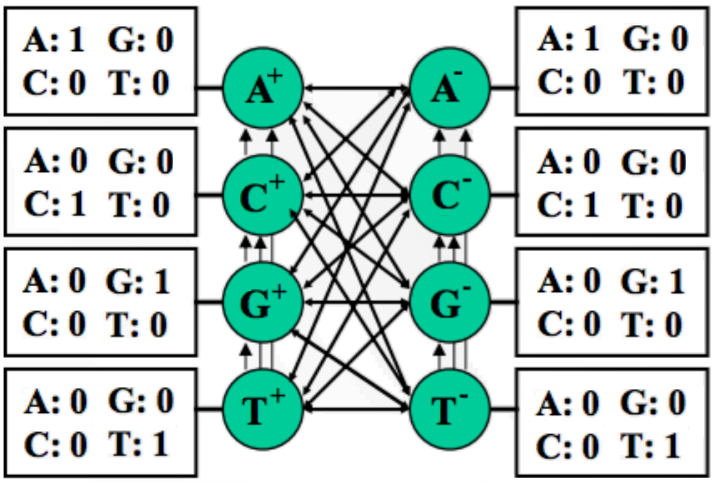
\includegraphics[width=.7\textwidth]{cg_stanja.png}
  \caption{Нова структура модела \textit{CG} острва \cite{kellis2021}}
  \label{fig:cg_stanja}
\end{figure}

Што се тиче почетних вероватноћа, могу се узети емпиријске, засноване на узорку, или пак равномерне могућности 1/8. Кад се све узме у обзир:
\begin{itemize}
  \item опсервације $y = \{A, C, G, T\}$ -- азбука ДНК нуклеотида,
  \item скривена стања $x = y \times \{+, -\}$ -- Декартов производ симбола,
  \item полазне вероватноће $\pi = \dfrac{1}{8}$ или емпиријске, према узорку,
  \item прелази $a =$ припремљене вредности према табели \ref{tab:cg_hmm1} или \ref{tab:cg_hmm2},
  \item емисије $b = 1$ ако стање одговара, иначе $0$, према слици \ref{fig:cg_stanja}.
\end{itemize}

И овакав модел даје врло добре резултате. Други приступ потрази за генима који укључује већи број стања и није заснован на проналажењу \textit{CG} острва. Алтернативна идеја заправо моделује сложенију структуру еукариотске ДНК, с циљем да још детаљније и прецизније анотира улазне секвенце.

Иако \textit{CG} острва јесу добар показатељ да се у близини налази неки промотер, који би могао да покрене преписивање (транскрипцију) гена, још би боље било када би се могло тачно одредити који нуклеотиди представљају ген, а који не. Познато је да се ДНК може поделити на више поднизова који имају двојаку природу -- или су интрони или егзони \cite{knapp2007, yoon2009}. Интрони су интрагенски региони, па тако представљају некодирајуће делове наследног материјала, који су уметнути између гена и који се уклањају у процесу сплајсовања. Егзони (ексони, због експресије), с друге стране, кодирају протеине, и увек су дужине дељиве са бројем три. Они се заправо састоје из триплета нуклеотида (кодона) који појединачно кодирају аминокиселине, које касније граде протеине. Постоји и неколико специјалних кодона -- почетни \textit{ATG} и завршни \textit{TAA}, \textit{TAG}, \textit{TGA} -- који означавају места на којима преписивање почиње и завршава се, мада стартни кодон на другим местима кодира метионин.

Последица је да се ДНК може моделовати и аутоматом са слике \ref{fig:eukariote}. На слици су представљени пример, стања и прелази, са већим бројем забрањених.

\begin{figure}[H]
  \centering
  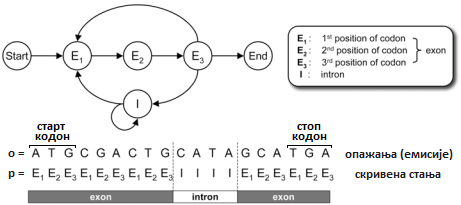
\includegraphics[width=.85\textwidth]{eukariote.png}
  \caption{Структура модела еукариотске ДНК \cite{eukary}}
  \label{fig:eukariote}
\end{figure}

Ово је, међутим, врло упрошћен модел, а у стварности је организација ДНК знатно комплекснија -- посебну структуру имају подланци на почетку и крају ДНК ланца, посебан удео нуклеотида имају делови на прелазу између егзона и интрона, а посебно се издвајају и такозвани \textit{ORF}-ови, који су целом дужином кодирајући, без интронских прекида \cite{henderson1997, huson2020}. Стога је очекивано да успешан модел ипак мора имати већи број стања, што и јесте случај.

Један од успешних модела за тачно предвиђање гена који кодирају протеине јесте \textit{GENSCAN}, алат који су 1997. године осмислили Берџ и Карлин \cite{genscan, burge1997}. Модел је карактеристичан по томе што предвиђа гене на оба ланца ДНК истовремено, па тако за већину елемената секвенце има дуплирана стања. Примера ради, делове егзона не моделује кроз три стања, као на слици \ref{fig:eukariote}, већ кроз шест. Укупно има 27 стања. Надограђен је појмом трајања (ново темпорално својство), по чему је такође карактеристичан, тако да није реч о сасвим обичном \textit{HMM}-у. Принцип рада је, међутим, исти: улаз је ДНК секвенца, а излаз декодирана стања, израчуната Витербијевим алгоритмом. Алат је прилично успешан, са стопом погодака од преко 90 \% по нуклеотиду и око 80 \% по егзону, о чему се детаљније може прочитати у цитираном раду.

За крај, корисно је сумирати успех \textit{HMM} у потрази за генима. Када се говори о моделима са само два стања (јесте или није \textit{CG} острво), проблематично је уколико се постави мала вероватноћа промене стања. Такав модел мале секвенце по правилу проглашава за целе (не)кодирајуће. С друге стране, повећањем вероватноће прелаза долази до извртања идеје, и тада само текући карактер постаје битан. Знатно побољшање добија се посматрањем динуклеотидног састава ниске, уместо скенирањем једног по једног карактера. Једнако добро се понаша модел са више стања, иако су му емисије дегенерисане.

Од свих разматраних модела је, међутим, најбоља надградња \textit{HMM} реализована кроз сложени алат \textit{GENSCAN}. Она можда не проналази \textit{CG} острва као таква, али зато прецизно лоцира кодирајуће егзоне. Општи закључак могао би бити да се боље показују модели са више стања, који конкретније хватају зависности. Штавише, овај проблем спада у оне поменуте у уводу, који се ефикасније могу решити помоћу многобројних надградњи \textit{HMM}. Једна од општијих успешних допуна јесу условна случајна поља, која умањују број погрешних предвиђања \cite{culotta2005, decaprio2007}.

% Profile HMMs for Sequence Alignment
\section{Профилни модели}
Крунско и можда најпознатије постигнуће скривених Марковљевих модела управо је њихова употреба у статистички поткованој класификацији секвенцијалних података. Конкретно, у наставку је размотрена примена у класификацији протеина, мада је објашњено и како се резултат уопштава.

Протеини су, наиме, организовани у разнолике протеинске фамилије, а чест биолошки задатак јесте додељивање новооткривеног полипептида некој од познатих фамилија. Замисао је да се на неки начин оцени припадност новог аминокиселинског ланца неким познатим фамилијама, а затим протеин додели оној са највећим скором. Наивни приступ оцењивању подразумева поређење улазног полипептида са сваким чланом фамилије појединачно, те напослетку сабирање тако добијених скорова или пак узимање максималног.

Протеини се у биоинформатици представљају својом примарном структуром, као ниска аминокиселина (азбука од двадесетак слова), па се међусобно могу лако поредити неким алгоритмом за рад са нискама. Често се, међутим, дешава да између појединих чланова фамилије постоје веће разлике, као нпр. код изузетно варијабилног гликопротеина \textit{gp120} код ХИВ-а, како је размотрено у уводу. То резултује веома малим скоровима, па стога поређење по паровима у општем случају не даје добре резултате.

Последица је да се протеин који се класификује мора поредити са целом фамилијом одједном. За те потребе, фамилије се најчешће представљају као вишеструка поравнања и изведене профилне матрице.

Подсећања ради, вишеструко поравнање је матрица карактера (низ ниски), чији редови представљају ниске које се поравнавају, а колоне карактере тих ниски на позицији одређеној том колоном. Како су при поравнању дозвољене инсерције (убацивање) и делеције (брисање слова), у нискама се налази и специјални карактер "--", који означава празнину. Није необично да постоје ретке колоне, у којима је велики удео празнина. Биолошки гледано, та аминокиселина вероватно није битна карактеристика фамилије која се моделује, па се занемарује. Прецизније, уклањају се све колоне у којима је удео празнина већи од унапред одређене границе $\theta$. Резултат је пречишћено поравнање.

Напослетку се пречишћено поравнање трансформише у профилну матрицу, чији редови представљају (све) карактере из азбуке поравнатих ниски, док колоне складиште удео сваког карактера на тој позицији, не рачунајући празнине. Приметно је да профил, како говори о вероватносној расподели по колони (позицији) карактера из азбуке $y$ величине $m$, веома личи на мапу емисија неког \textit{HMM}-а. Испоставља се да се стварно може тако посматрати.

Најједноставнији \textit{HMM} за моделовање фамилија протеина могао би бити у суштини дегенерисан ланац скривених стања $x$, такав да свако стање представља једну позицију, којих је укупно $n$. Од сваког стања $x_i$ постоји само један прелаз са јединичном вероватноћом на стање $x_{i+1}$, док се вероватноће емисија узимају из профила. Прво стање $x_1$ обавезно је почетно, док је последње $x_n$ обавезно завршно. На слици \ref{fig:profil} приказан је претходно изнети ток догађаја од вишеструког поравнања до ланчаног \textit{HMM}-а. Полазно има десет позиција, које се границом одсецања $\theta =$ 0,35 своде на коначних осам.

\begin{figure}[H]
  \centering
  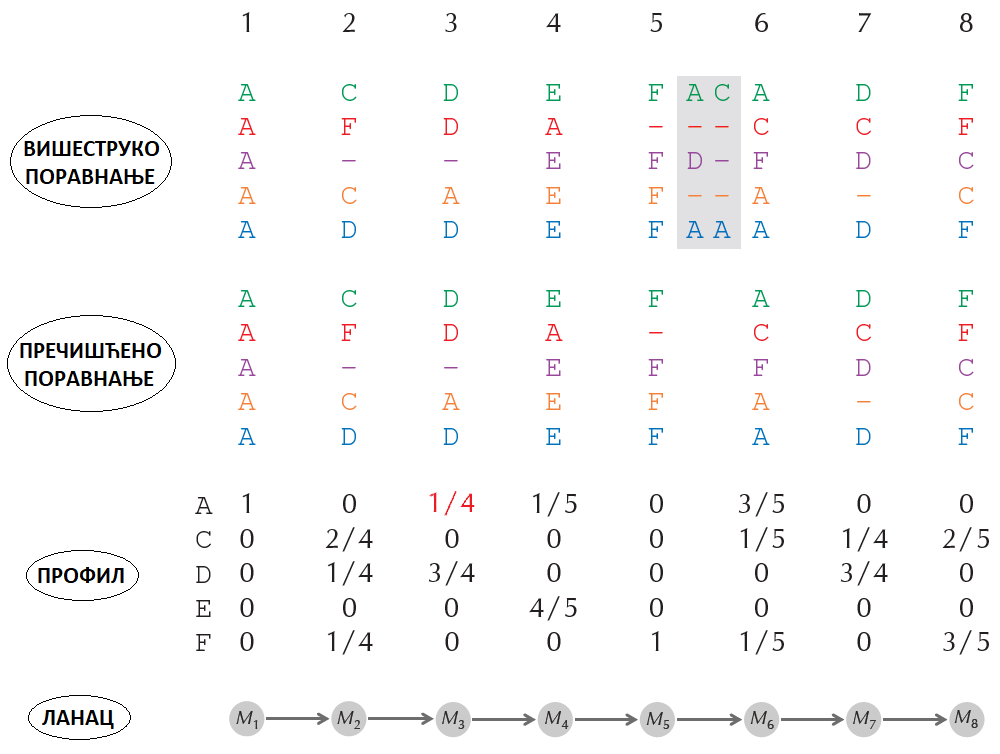
\includegraphics[width=\textwidth]{profil.png}
  \caption{Мотивациони пример \textit{HMM} профила \cite{compeau2015}}
  \label{fig:profil}
\end{figure}

Ваља напоменути да се стања ланчаног \textit{HMM}-а најчешће означавају као $M_i$, како је и на слици, а не као $x_i$, како је уобичајено код \textit{HMM}. Разлог томе је што она заправо представљају поклапања (енгл. \textit{Match}) на тој позицији. Напоменуто је већ и да је овакав модел дегенерисан. Како има обавезно почетно и завршно стање, као и обавезне прелазе, кроз њега постоји само један скривени пут -- тачно $M_1M_2...M_{n-1}M_n$.

Остаје још питање употребне вредности оваквог модела, односно оваквих модела, јер би постојао по један \textit{HMM} за сваку фамилију. Сада би се скор могао добити као вероватноћа емитовања ниске (новог полипептида) $o$ у осмишљеном моделу. И овога пута, протеин би био додељен оној фамилији са највећим $P\{o\}$. Одређивање те вероватноће већ је разматрано као решење проблема \ref{prob:ops}. Ипак, како је модел дегенерисан, нема потребе примењивати сложени алгоритам "напред", па чак ни рачунати једнаку вероватноћу при обавезном путу $P\{o | M_1...M_n\}$, као решење проблема \ref{prob:ishod}. Довољно је само помножити одговарајуће вредности из профилне матрице. Примера ради, вероватноћа да \textit{HMM} са слике \ref{fig:profil} емитује $ADDAFFDF$ износи (слика \ref{fig:prof_ishod}): $$P\{ADDAFFDF\} = 1 \cdot \frac{1}{4} \cdot \frac{3}{4} \cdot \frac{1}{5} \cdot 1 \cdot \frac{1}{5} \cdot \frac{3}{4} \cdot \frac{3}{5} = 0,003375.$$

\begin{figure}[H]
  \centering
  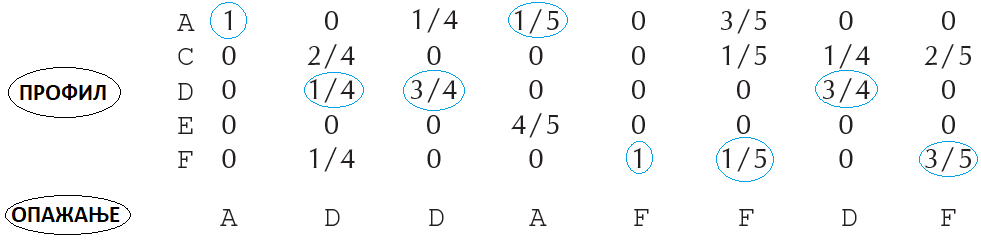
\includegraphics[width=\textwidth]{prof_ishod.png}
  \caption{Вероватноћа опсервације као скор фамилије \cite{compeau2015}}
  \label{fig:prof_ishod}
\end{figure}

Свеукупно, овакав модел није лош утолико што добро осликава сличност протеина са фамилијом -- што је улазни полипептид сличнији фамилији, то је његов скор (вероватноћа) већи. Такође, различито оцењује сваку појединачну колону, што је циљ постављен у уводу. Ипак, он због дегенерисаности и није прави \textit{HMM}. Штавише, није ништа бољи од саме профилне матрице. Иако је употребљив за опсервације (полипептиде) дужине $k = n$, главно ограничење је што се лоше моделују исходи других дужина. Њихова вероватноћа је подразумевано нулта, тј. сматрају се немогућим. Овај наивни модел, ипак, није толико бескористан, јер се може употребити као основа за прављење напредног, свеобухватног \textit{HMM}-а за класификацију разних врста секвенцијалних података, а не само протеина, о чему ће бити речи у наставку.

Прво, могуће је суочити се са проблемом опажања дужине $k > n$. Једноставно решење јесте додавање нових стања, која би дозволила додатне приказе. Прецизније, најбоље је додати $n+1$ стање инсерције $I_i$, за индекс $i \in \{0, ..., n\}$. Замисао је да посета стању $I_i$ дозволи емитовање додатних симбола између колона $i$ и $i+1$ поравнања. Стога се додају гране од $M_i$ ка $I_i$, као и од $I_i$ ка $M_{i+1}$. Наравно, како би било могуће емитовати више додатних симбола, додаје се и петља -- грана од $I_i$ ка самом себи. Специјално, стање $I_0$ моделује инсерције пре првог карактера поравнања, док $I_n$ дозвољава уметања након последњег слова. Слика \ref{fig:insercije} приказује употребу нових стања у одређивању пута кроз дорађени ланац са слике \ref{fig:profil} за досад необјашњиво опажање $A\textcolor{red}{F}DDAFFDF$. Ово је, дакле, опажање $ADDAFFDF$ са слике \ref{fig:prof_ishod}, али уз уметнутно $F$ на другом месту. Оптимални пут је подебљан.

\begin{figure}[H]
  \centering
  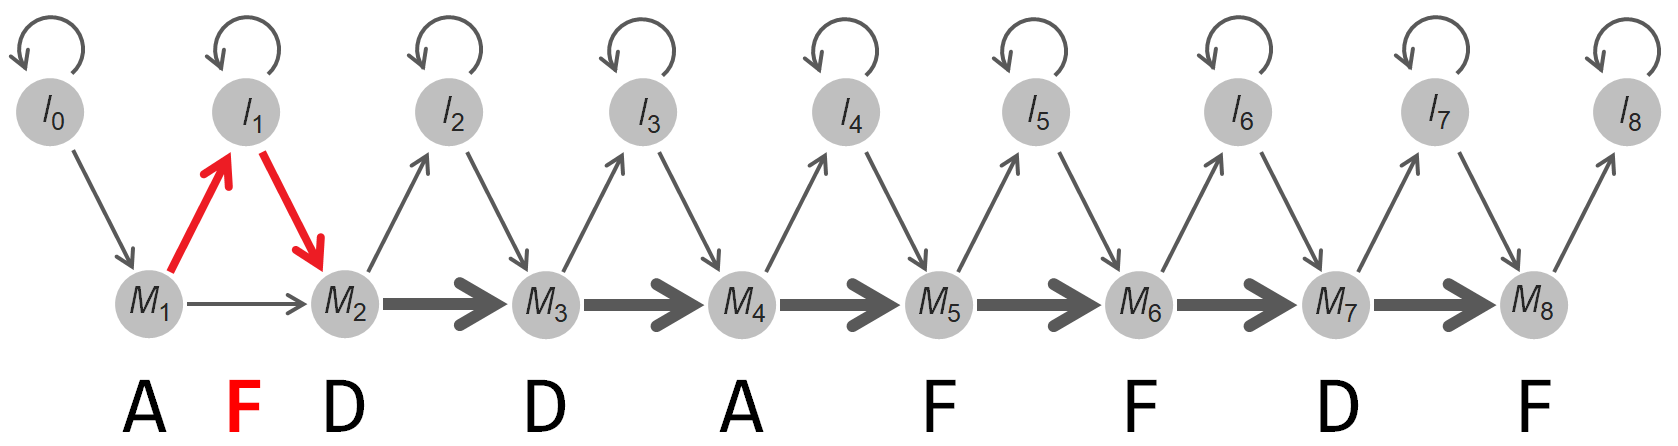
\includegraphics[width=\textwidth]{insercije.png}
  \caption{Увођење стања инсерције \cite{compeau2015}}
  \label{fig:insercije}
\end{figure}

Даље, могуће је ухватити се укоштац и са проблемом опажања дужине $k < n$. Сада је задатак моделовати делеције, односно омогућити прескакање неких колона поравнања. Наиван приступ овом решењу било би баш прескакање неких поклапања додавањем великог броја грана. Наиме, могла би се додати по грана ка сваком $M_i$ од сваког $M_j$ и $I_j$ за $j < n$, као и по једна од сваког $M_i$ ка сваком $M_j$ и $I_j$ за $j > n$. Другим речима, тада би се у неко стање поклапања могло непосредно доћи из било ког стања лево, као и непосредно отићи у било које стање десно. Како би то изгледало на дорађеном моделу са слике \ref{fig:insercije}, може се видети на слици \ref{fig:delecije1}, која следи. Црвеном бојом наглашена је грана која омогућује рад са досад необјашњивим опажањем $AAFFDF$, дакле са уклоњена два карактера $DD$. Како би слика остала читљива, додате су само нове гране чији је један крај поклапање $M_4$.

\begin{figure}[H]
  \centering
  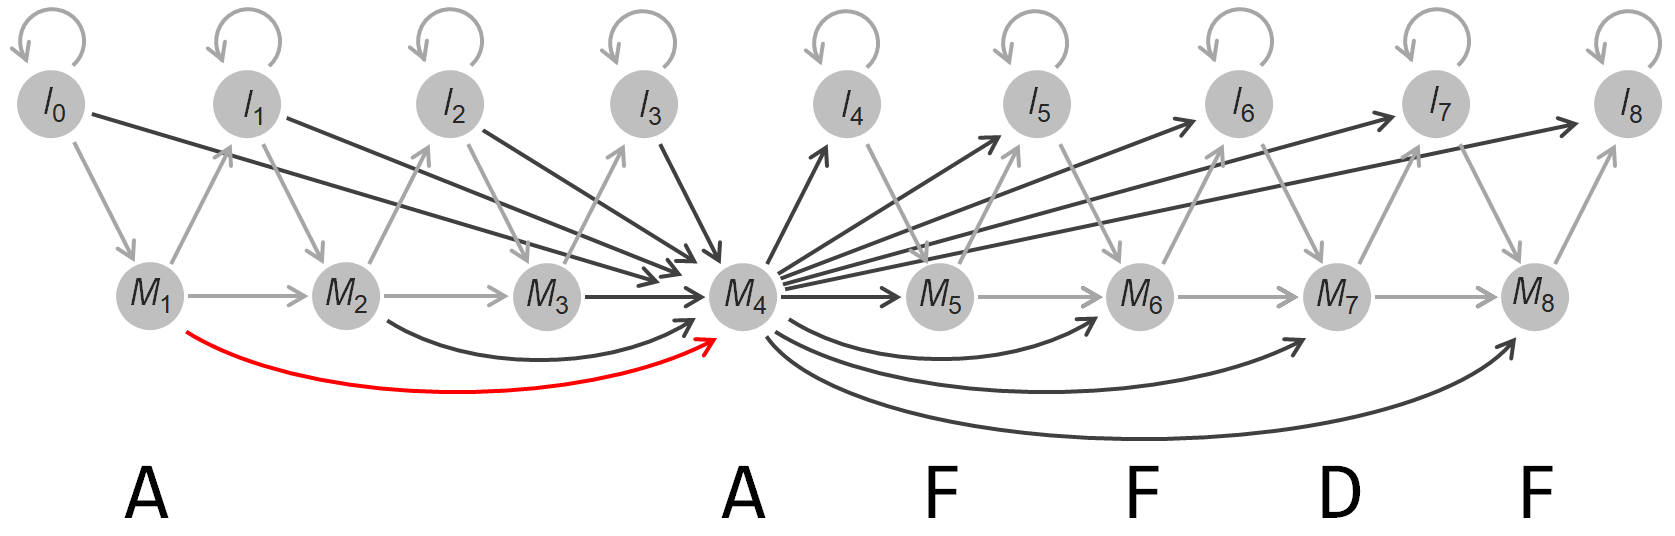
\includegraphics[width=\textwidth]{delecije1.png}
  \caption{Наивна обрада делеција \cite{compeau2015}}
  \label{fig:delecije1}
\end{figure}

Овакав приступ, међутим, није пожељан, управо због великог броја додатих грана. Подсећања ради, сви важни алгоритми за рад са \textit{HMM} засновани су на Витербијевом графу. Када се говорило о томе, напоменуто је да је сложеност Витербијевог и повезаних алгоритама директно сразмерна броју грана у графу, који, с друге стране, зависи од броја дозвољених прелаза у самом моделу. Претходном дорадом, број прелаза је са линеарног скочио на квадратни -- реда $O(n^2)$, где $n$, као и досад, означава број колона у поравнању.

Како би рад са моделом био ефикасан, неопходно је задржати линеаран број грана. То се чини додавањем нових, тихих стања, која не приказују ништа (понекад се замшља да емитују празнину "--"), а представљају алтернативан пут у односу на главни, који иде преко стања поклапања. Прецизније, додаје се $n$ стања делеције $D_i$, таквих да се од сваког $D_i$ може доћи до $M_{i+1}$ и $D_{i+1}$, као и од сваког $M_i$ до $D_{i+1}$. Сада је колону поравнања $i$, односно стање $M_i$, могуће прескочити проласком кроз стање $D_i$. Слика \ref{fig:delecije2} приказује употребу нових стања у одређивању пута кроз дорађени модел са слике \ref{fig:insercije} за већ разматрано опажање $AAFFDF$. Оптимални пут је и сада подебљан.

\begin{figure}[H]
  \centering
  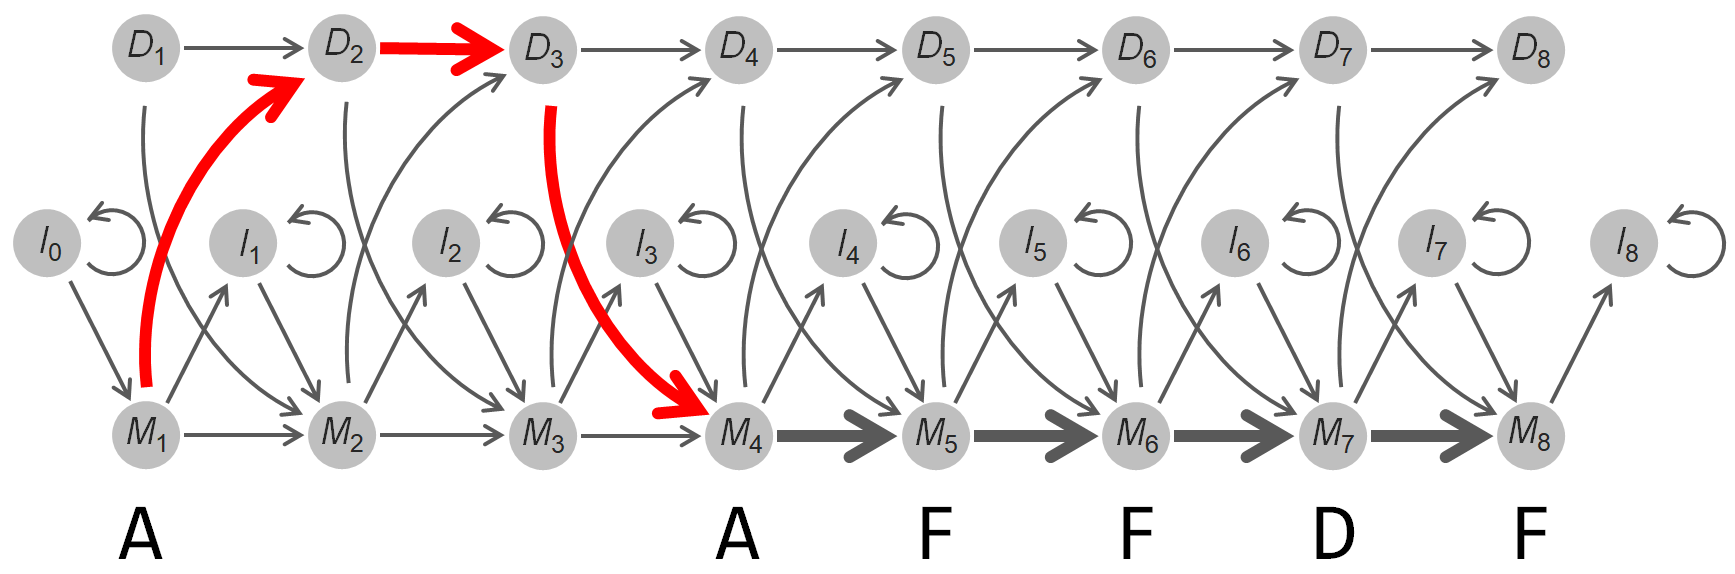
\includegraphics[width=\textwidth]{delecije2.png}
  \caption{Увођење стања делеције \cite{compeau2015}}
  \label{fig:delecije2}
\end{figure}

Сада су могући прелази између стања поклапања и инсерције, као и између стања поклапања и делеције. Како би модел био комплетан, недостају још прелази између инсерција и делеција. Конкретно, треба омогућити прелаз из сваког $D_i$ на $I_i$, као и од сваког $I_i$ ка $D_{i+1}$. Сада је могуће произвољно мењати тип стања: од инсерције $I_i \mapsto I_i$, $I_i \mapsto D_{i+1}$, $I_i \mapsto M_{i+1}$, од делеције $D_i \mapsto I_i$, $D_i \mapsto D_{i+1}$, $D_i \mapsto M_{i+1}$, од поклапања $M_i \mapsto I_i$, $M_i \mapsto D_{i+1}$, $M_i \mapsto M_{i+1}$. Коначна структура модела са осам колона пречишћеног вишеструког поравнања, који одговара мотивационом примеру, дата је на слици \ref{fig:indeli}.

\begin{figure}[H]
  \centering
  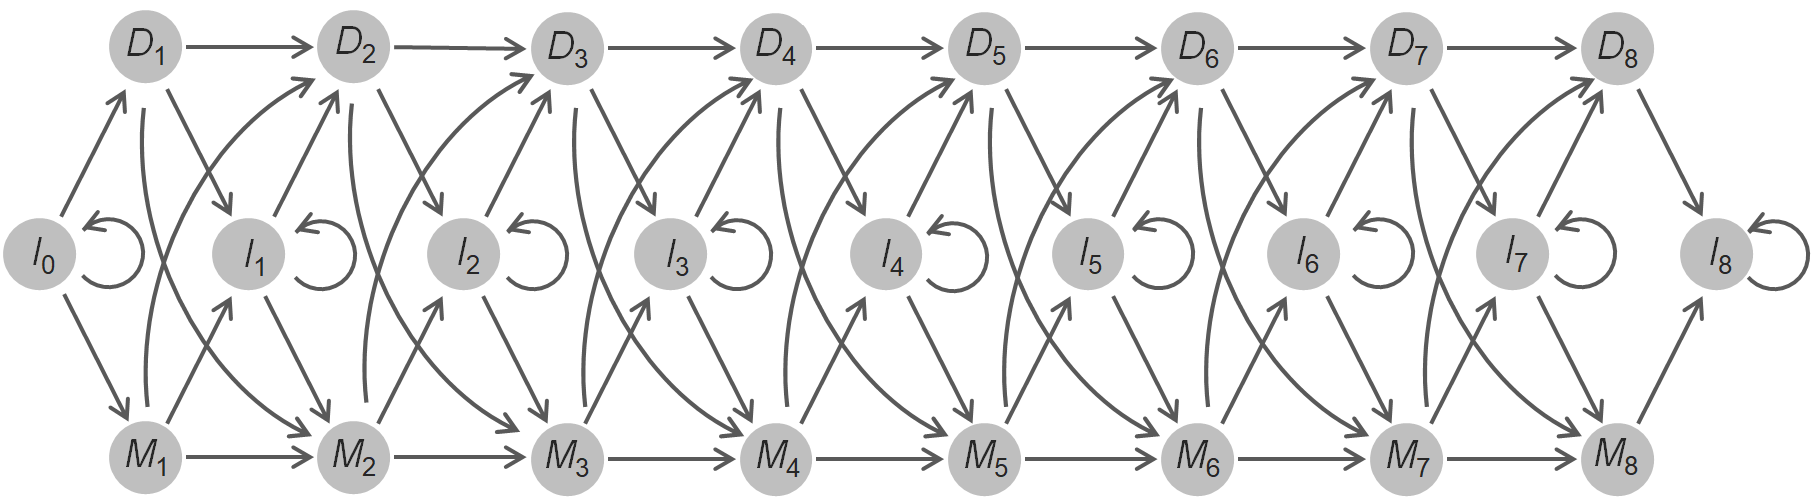
\includegraphics[width=\textwidth]{indeli.png}
  \caption{Коначна структура модела \cite{compeau2015}}
  \label{fig:indeli}
\end{figure}

Већ је примећено да се код профилних модела са $n$ не означава број скривених стања, већ број колона пречишћеног вишеструког поравнања. Стања је трипут више. Још једна њихова специфичност је да је уобичајен рад са експлицитним почетним стањем $S$ (од енгл. \textit{Start}) и завршним $E$ (од енгл. \textit{End}), тако да се и она додају. Од полазног стања могуће је ући у $I_0$, $D_1$ или $M_1$, док се у терминално долази из $I_n$, $D_n$ или $M_n$. Свеукупно, општи профилни \textit{HMM} са $n$ колона могао би се приказати дијаграмом са слике \ref{fig:prof_hmm}.

\begin{figure}[H]
  \centering
  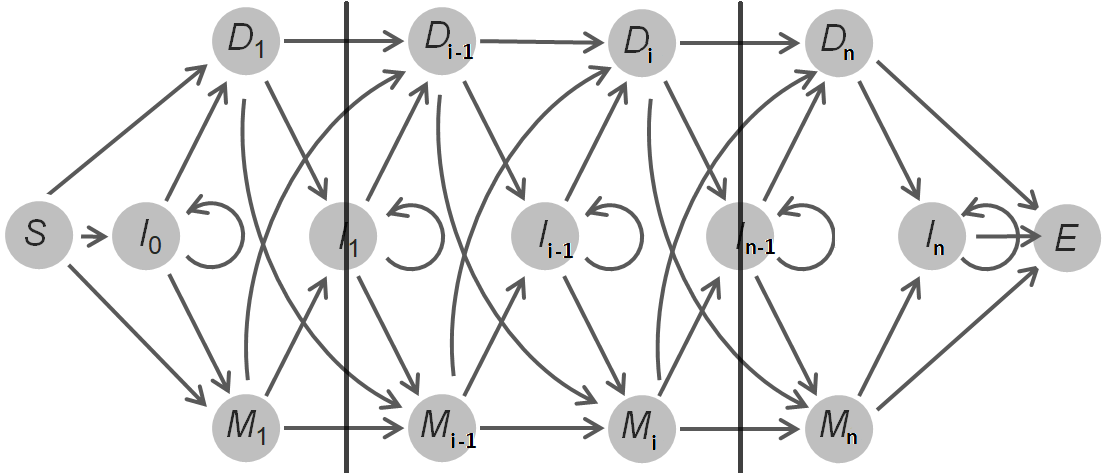
\includegraphics[width=.95\textwidth]{prof_hmm.png}
  \caption{Општи профилни \textit{HMM}}
  \label{fig:prof_hmm}
\end{figure}

Ово је, дакле, такозвани профилни \textit{HMM} или \textit{HMM} профил. Историјски гледано, употребу оваквих модела описали су 2002. Бејтман и сарадници, на основу чега је осмишљена позната база података Пфам \cite{bateman2002}. Она се данас састоји од скоро 20.000 вишеструких поравнања разних протеинских домена (издвојени делови протеина, попут \textit{V3} петље из увода) и рутински се користи у анализи нових протеинских секвенци \cite{pfam}. Како се граде на основу поравнања $P$ и границе одсецања $\theta$, профили се означавају као $HMM(P, \theta)$. Њихово одређивање формално се представља кроз проблем \ref{prob:prof}.

\begin{problem}[H]
  \SetAlgoLined
  \textit{Направити профилни \textit{HMM} на основу вишеструког поравнања.}\\
  \textbf{Улаз}: вишеструко поравнање $P$ и граница одсецања $\theta$.\\
  \textbf{Излаз}: профилни модел $HMM(P, \theta)$.
  \caption{Одређивање профилног модела \cite{ba10e}}
  \label{prob:prof}
\end{problem}

Подсећања ради, сваки \textit{HMM} је петорка, а засад је одређен само први члан -- скривена стања $x$, којих је укупно $3n+3$. Одређен је и скуп дозвољених прелаза, па тако из сваког стања излазе највише по три гране, што значи да је укупан број прелаза линеаран -- реда $O(n)$, како је и захтевано. Могуће опсервације, као други члан петорке, познате су из улазног поравнања, а зависе од примене. У случају рада са протеинима, скуп $y$ гради двадесетак аминокиселина. Из профилне матрице су познате и емисије у стањима поклапања, а познати су и обавезно почетно (трећи члан петорке $\pi$) и завршно стање.

Недостају, међутим, све вероватноће прелаза $a$, као и расподела опажања $b$ у непоклапајућим стањима. Њихово одређивање илустровано је сликом \ref{fig:prof_param}.

\begin{figure}[H]
  \centering
  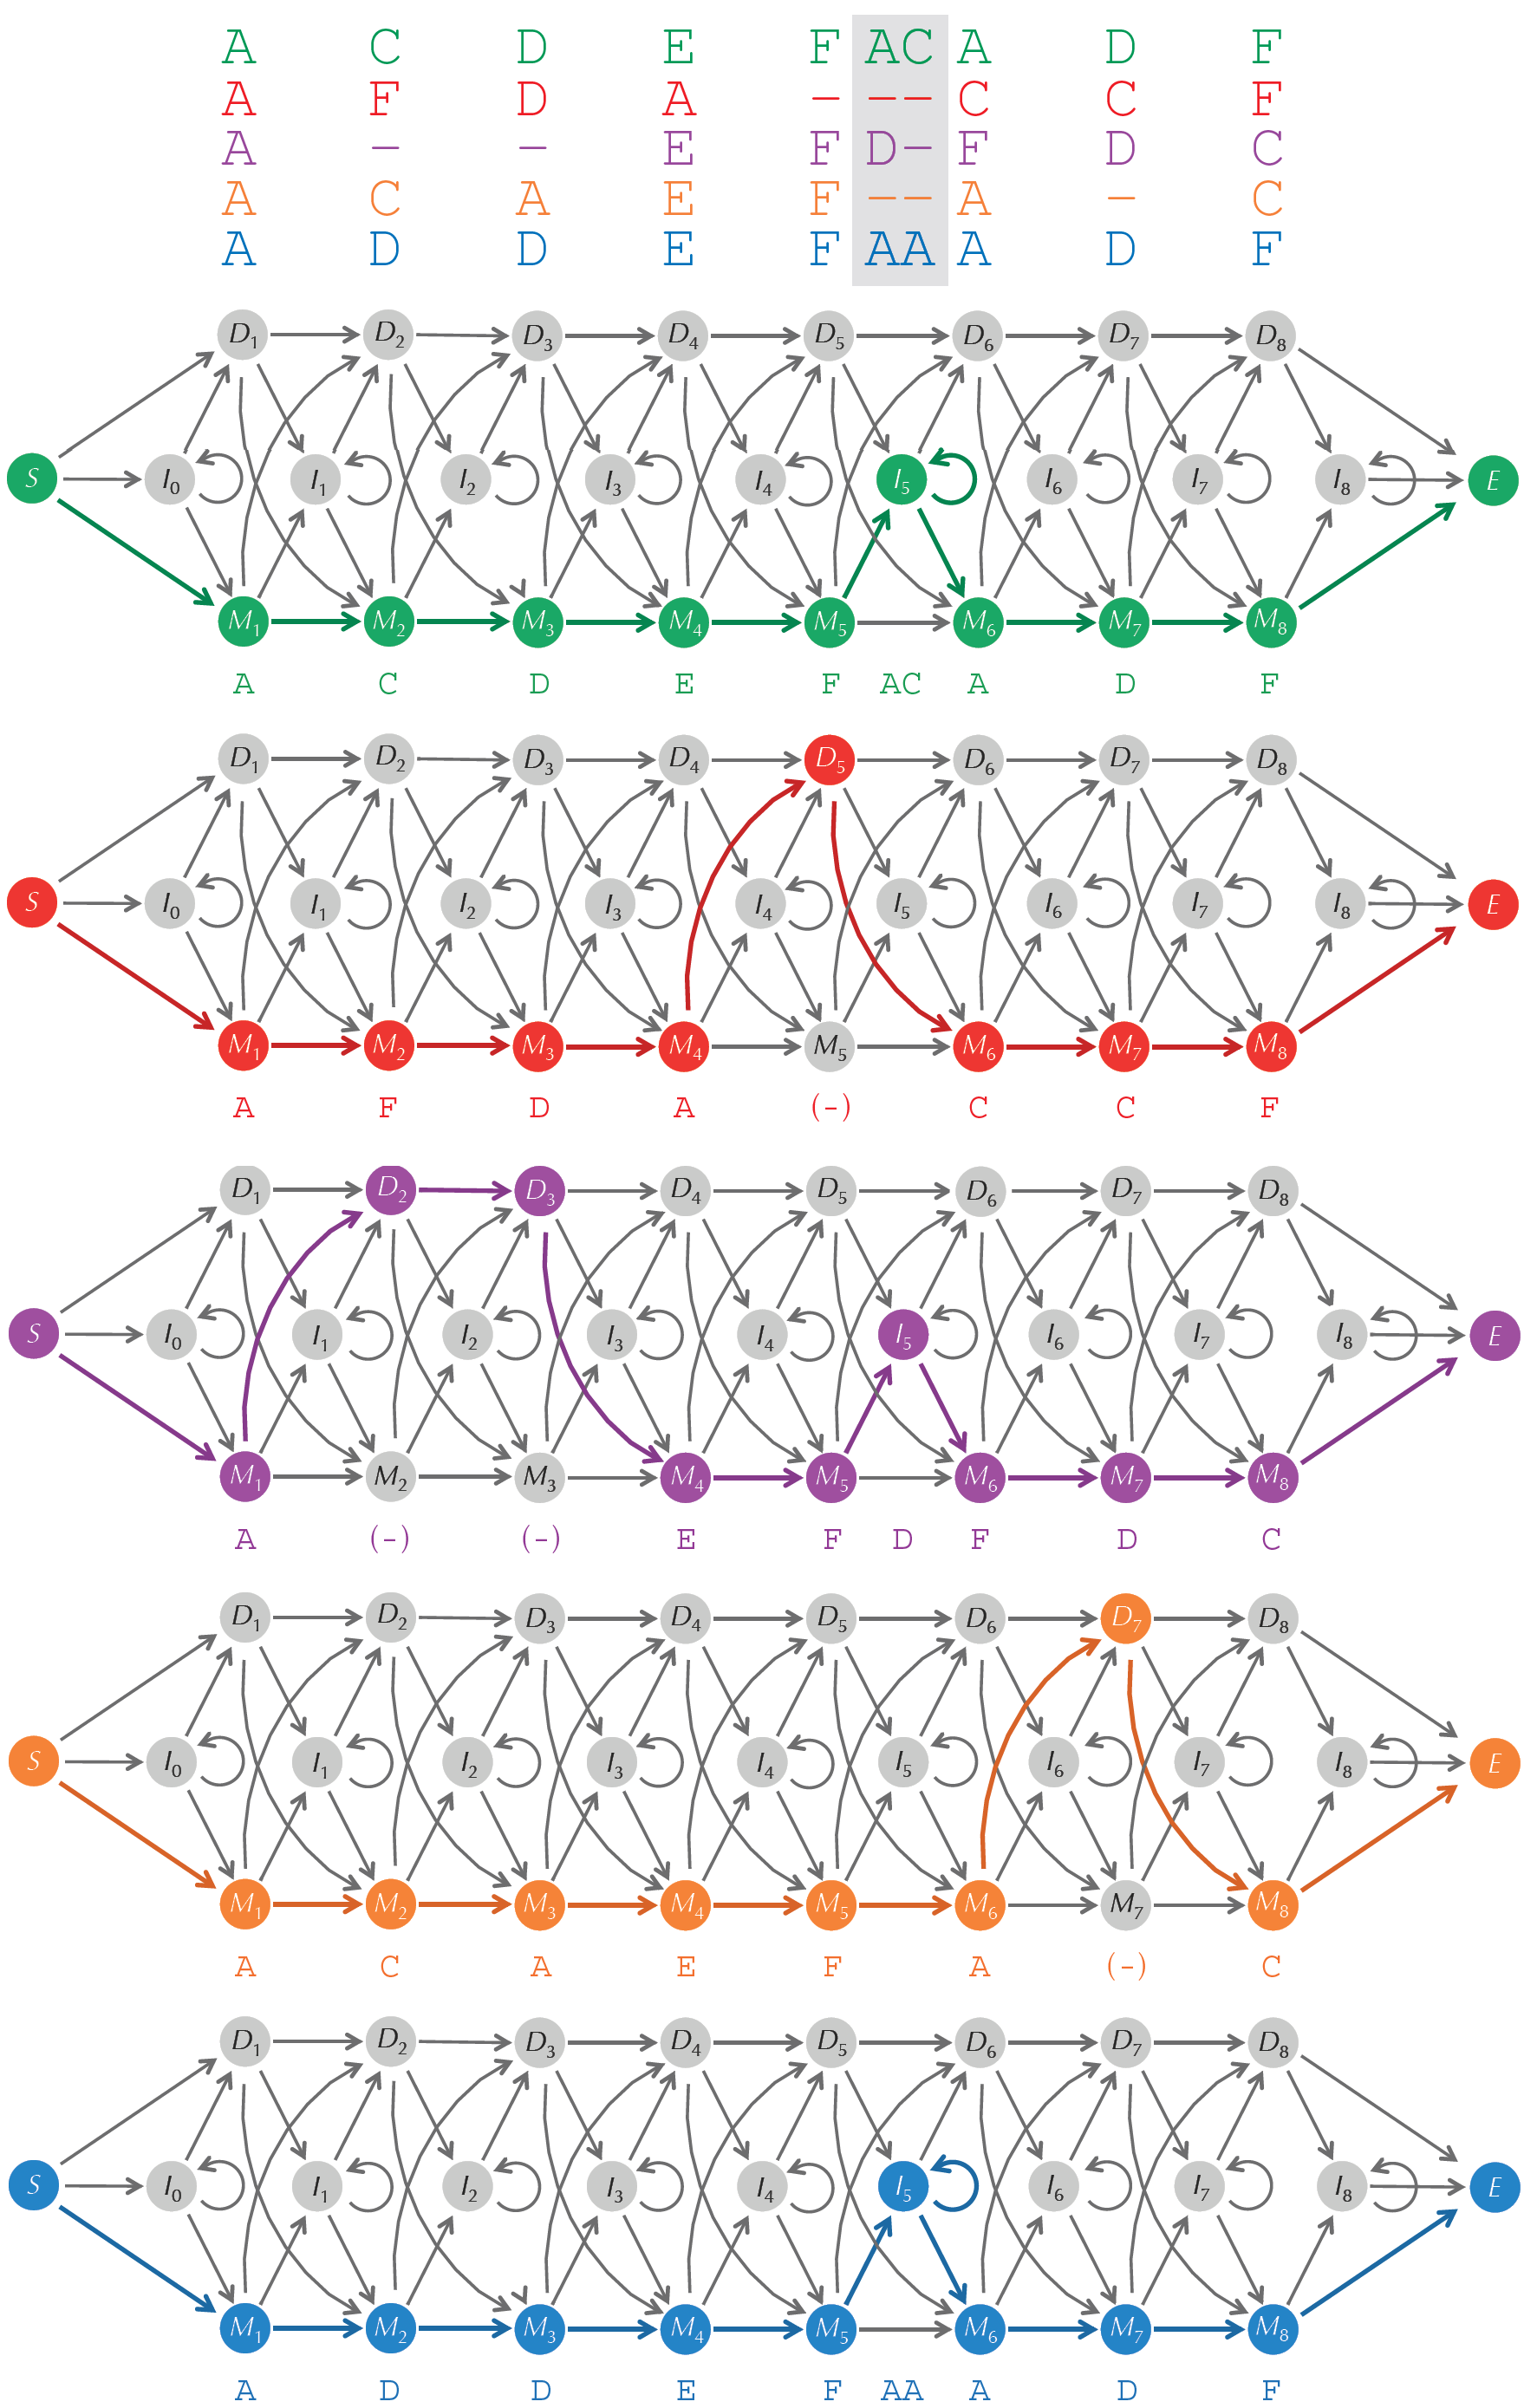
\includegraphics[height=.97\textheight]{prof_param.png}
  \caption{Одређивање параметара профилног \textit{HMM} \cite{compeau2015}}
  \label{fig:prof_param}
\end{figure}

% Classifying proteins with profile HMMs
\section{Рад са профилима}
Вероватноће се рачунају емпиријски, на основу улазног вишеструког поравнања. Претходна слика сваку од обојених ниски из поравнања (исти мотивациони пример као и досад, са прве слике \ref{fig:profil}) приказује као оптимални пут исте боје кроз профилни \textit{HMM}. Веза између ниске као реда вишеструког поравнања и оптималног пута кроз профилни \textit{HMM} једнозначна је. Уколико се у задржаној колони (чиста позадина) $i$ налази емитовани симбол, пролази се кроз стање поклапања $M_i$. Ако задржана колона $i$ складишти празнину "--", пролази се кроз стање делеције $D_i$. Празнина се у пречишћеној колони (осенчена позадина) која се налази између задржаних колона $i$ и $i+1$ занемарује, док емитовани симболи означавају пролазак кроз стање инсерције $I_i$.

На основу одређених скривених путева, могуће је простим бројањем одредити колико често долази до неког прелаза, те расподелу емисија по сваком стању. Нека се разматра пример са слике \ref{fig:prof_param}, који садржи пет путева. Четири пута -- сваки сем црвеног -- пролазе кроз стање $M_5$. Од њих, један пут -- наранџасти -- наставља у стање $M_6$, док преостала три одлазе у стање $I_5$. Овиме је одређена фреквенција дозвољених прелаза, па су вероватноће: $$a_{M_5, I_5} = \frac{3}{4}, a_{M_5, D_6} = 0, a_{M_5, M_6} = \frac{1}{4}.$$

Аналогно се одређују вероватноће прелаза између осталих стања, укључујући специјално полазно и завршно. Ако емпиријски путеви не покривају све прелазе, као између $M_5$ и $D_6$, што је сасвим уобичајено, вероватноћа прелаза сматра се непознатом, односно она је имплицитно нулта (недозвољени прелаз). Ово је један од примера када мапе не покривају цео простор вероватноћа, односно оне се не сумирају у јединицу, иако би то било очекивано.

И вероватноће опажања одређују се фреквенцијски. На примеру стања $M_5$, у сва четири пролаза емитован је симбол $F$. Стога је мапа следећа: $$b_{M_5, A} = b_{M_5, B} = b_{M_5, C} = b_{M_5, D}= b_{M_5, E} = 0, b_{M_5, F} = \frac{4}{4} = 1.$$ Такође постоји доста непознатих емисија, па је удео имплицитних нула велик.

Приметно је да је у добијеним мапапа значајан број непознатих вредности, што онемогућава добро оцењивање великог броја секвенци чије би декодирање ишло тим путевима. Њихова вероватноћа била би нула, што је проблем по ком тренутни модел личи на полазни ланац. Да је стварно тако, показује резултујућа мапа прелаза мотивационог примера, приказана на слици \ref{fig:prelazi}.

\begin{figure}[H]
  \centering
  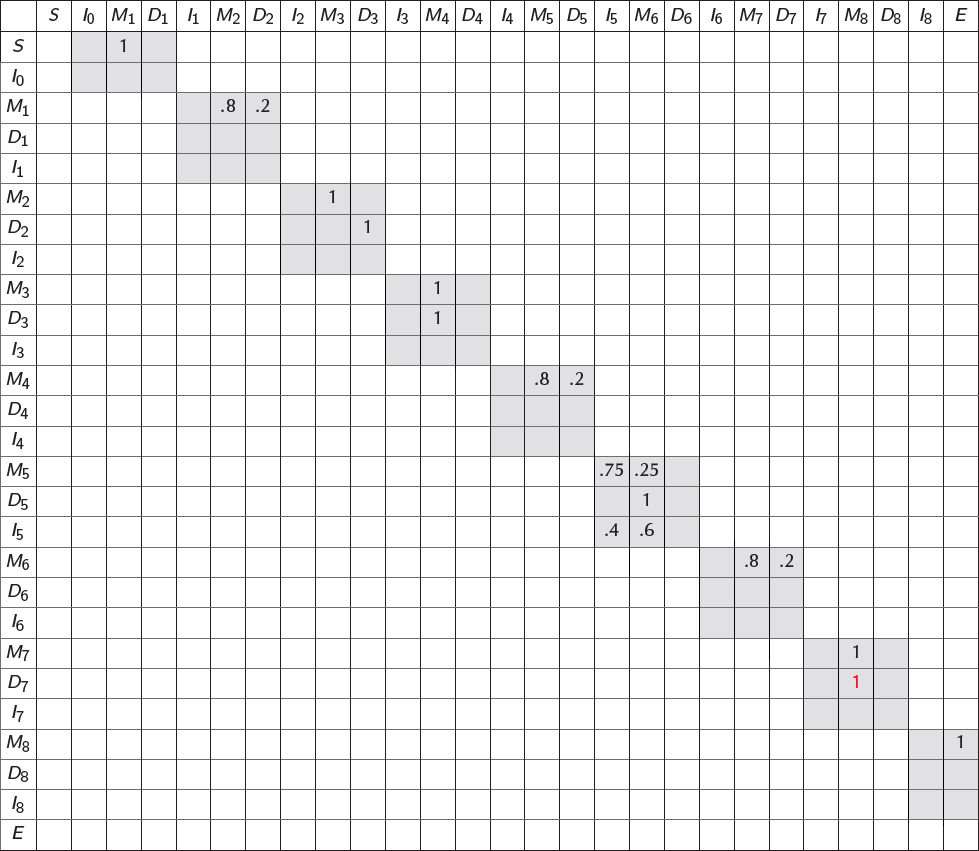
\includegraphics[width=\textwidth]{prelazi.png}
  \caption{Вероватноће прелаза мотивационог примера \cite{compeau2015}}
  \label{fig:prelazi}
\end{figure}

Моделом недозвољени прелази, попут $M_1 \mapsto M_5$, илустровани су ћелијама чисте позадине, док су могући прелази осенчени. Приметно је да је од укупно 75 дозвољених прелаза, само 19 евалуирано, док је преостала већина непозната -- оне су имплицитно нулте. Како ово није пожељна особина, у наставку је превазиђено употребном малих вероватноћа за непознате прелазе.

Поменуто је већ да је главни проблем који то изазива лоше оцењивање многих секвенци и путева. Конкретан пример дат је у наставку. Други проблем је што овакве мапе не покривају цео простор вероватноћа, односно не сумирају се све излазне вероватноће у јединицу. Све ово се, међутим, лако превазилази увођењем псеудовредности $\sigma$, што су мале вероватноће дозвољених, али често непознатих прелаза и емисија. Оне се, дакле, додају у мапама на сва дозвољена места.

Наравно, приликом додавања псеудовредности неопходно је применити нормализацију, како би збир вероватноћа био један. Примера ради, за $\sigma = 1/100$, ред \{.75, .25, 0\} не постаје \{.76, .26, .01\}, већ \{.738, .252, .01\}. Исто тако, сасвим непознати ред \{0, 0, 0\} за свако $\sigma$ постаје \{1/3, 1/3, 1/3\}, уместо \{1/100, 1/100, 1/100\} у конкретном случају. Такође, важно је напоменути да се псеудовредности додају искључиво дозвољеним прелазима, док недозвољени остају строго нулте вероватноће. Одређивање овако допуњеног профилног модела $HMM(P, \theta, \sigma)$ формално се представља кроз проблем \ref{prob:prof_sigma}.

\begin{problem}[H]
  \SetAlgoLined
  \textit{Направити профилни \textit{HMM} на основу вишеструког поравнања.}\\
  \textbf{Улаз}: поравнање $P$, граница $\theta$, псеудовредност $\sigma$.\\
  \textbf{Излаз}: дорађени профилни модел $HMM(P, \theta, \sigma)$.
  \caption{Одређивање дорађеног профилног модела \cite{ba10f}}
  \label{prob:prof_sigma}
\end{problem}

Овиме је појам профилног скривеног Марковљевог модела комплетиран. Идеја оваквог модела заправо је двојака. Први циљ је већ поменута класификација, која улазу додељује скор припадности одређивањем вероватноће исхода (алгоритам "напред"). Додатно, могуће је одредити и само поравнање ниски са представљеном фамилијом, које се добија декодирањем улаза (Витербијев алгоритам).

О класификацији је већ било речи -- одредити вероватноћу да протеин припада неким фамилијама, а затим га доделити оној са највећим скором или макар скором који прелази постављену границу. На конкретном примеру предвиђања фенотипа ХИВ-a из увода, могла би постојати два \textit{HMM} профила -- један изграђен на основу изолата који стварају синцицијум, а други према оним који га не стварају. Нов изолат за који је упитно ствара ли синцицијум био би улазно опажање за алгоритам "напред" над та два профила, а одговор на питање добио би се одабиром профила са већом вероватноћом.

Одабрани профил се, штавише, опционо може проширити додавањем новог изолата у поравнање, а затим поновним израчунавањем параметара тог \textit{HMM}-а. Ажурирањем профила, он временом све боље описује класу коју моделује, те постаје још прецизнији и употребљивији при класификацији.

Овакав принцип може се уопштити на све друге секвенцијалне податке. Прави се, дакле, по један \textit{HMM} профил за сваку могућу класу, а затим се профили пореде са улазном секвенцом, која се класификује. Инстанци се додељује она класа са највећом вероватноћом опажања. За рад са генима и протеинима, на интернету је бесплатно доступан претраживач \textit{HMMER} \cite{hmmer}, управо заснован на припремљеним скривеним Марковљевим моделима.

Што се тиче другог циља, поравнање ниске са профилом добија се непосредно као резултат декодирања. Пример тога дат је на слици \ref{fig:poravnanje}.

\begin{figure}[H]
  \centering
  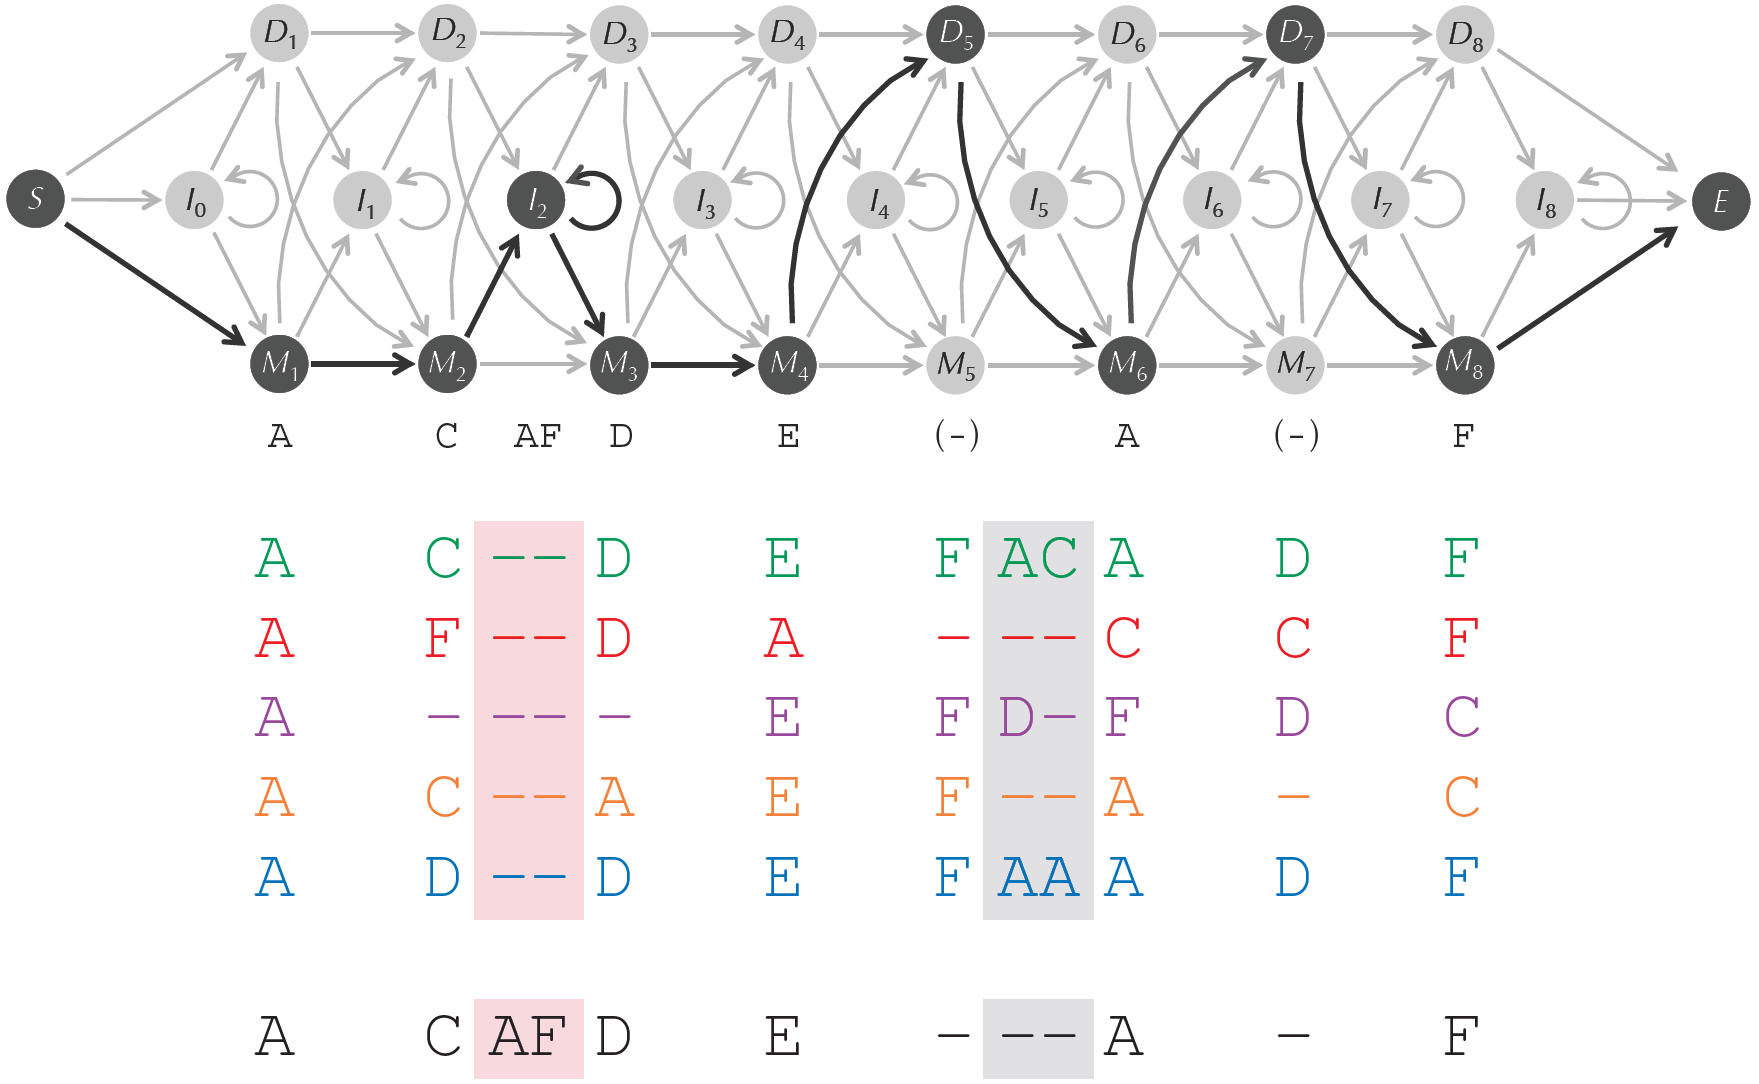
\includegraphics[width=\textwidth]{poravnanje.png}
  \caption{Пример поравнања мотивационог примера \cite{compeau2015}}
  \label{fig:poravnanje}
\end{figure}

Приказан је оптимални пут $S M_1 M_2 I_2 I_2 M_3 M_4 D_5 M_6 D_7 M_8 E$ кроз досад разматрани профилни \textit{HMM} за ниску (опажање) $ACAFDEAF$. Ваља приметити да је овај пут иначе немогућ (нулте вероватноће) без употребе псеудовредности, јер је нпр. вероватноћа прелаза $M_2 \mapsto I_2$ непозната, па самим тим имплицитно нулта без неког $\sigma$. У бојама је, као и досад, приказана петорка из почетног вишеструког поравнања, док је ниска која се поравнава црна.

Конкретно, заједнично вишеструко поравнање је следеће. Прва два симбола емитована су из стања поклапања $M_1$ и $M_2$, тако да се налазе у првој, односно другој колони поравнања. Следећа два симбола емитована су из стања инсерције $I_2$, тако да се налазе између друге и треће колоне, што је назначено розе сенком. Како је то посебан додатак за нову ниску, полазној петорци једноставно се додају по две празнине. Наредна два симбола емитована су из стања поклапања $M_3$ и $M_4$, тако да се налазе у трећој, односно четвртој колони поравнања. Следеће на путу јесте тихо стање делеције $D_5$, тако да нема емисије, већ се у пету колону поравнања ставља симбол празнине "--". Наредни симбол емитован је из стања поклапања $M_6$, па се ставља у шесту колону поравнања. Пре њега није било инсерција, тако да се две пречишћене колоне попуњавају празнинама. Следи тихо стање делеције $D_7$, што значи да се у седму колону ставља празнина, док је последњи симбол емитован из стања поклапања $M_8$, те се ставља у осму колону поравнања.

Како би поравнање било добро одређено, неопходно је пратити текући карактер нове ниске која се поравнава са фамилијом, односно кренути од првог слова и померати "показивач" када дође до емисије. Општа правила поравнавања сумирају се следећим списком смерница за тумачење стања оптималног скривеног пута:
\begin{itemize}
  \item пролазак кроз стање поклапања $M_i$ заправо представља емитовање текућег симбола, те поставља тај симбол управо у колону $i$ поравнања,
  \item пролазак кроз стање инсерције $I_i$ такође представља емитовање текућег симбола, али поставља тај симбол између колона $i$ и $i+1$ поравнања,
  \item пролазак кроз стање делеције $D_i$ оставља текући симбол на чекању, те поставља алтернативни симбол празнине "--" у колону $i$ поравнања.
\end{itemize}
Поравнање је смислено уколико су проласком кроз скривени пут потрошени сви карактери улазног опажања, што се осигурава позадинским алгоритмом. Такође, уколико је циљ истовремено поравнање и са оригиналним и са пречишћеним вишеструким поравнањем, као на слици \ref{fig:poravnanje}, неопходно је посебно пазити да ли се прелази преко пречишћеног дела (сиво сенчење). Ипак, углавном је довољно поравнати ниску само са пречишћеном верзијом.

Остаје још питање како тачно наћи оптимални скривени пут. Јасно је да се може применити Витербијев алгоритам, који је досад коришћен за проблем декодирања. На слици \ref{fig:prof_vit} приказан је Витербијев граф и одговарајући скривени пут за љубичасто опажање $AEFDFDC$ из мотивационог примера.

\begin{figure}[H]
  \centering
  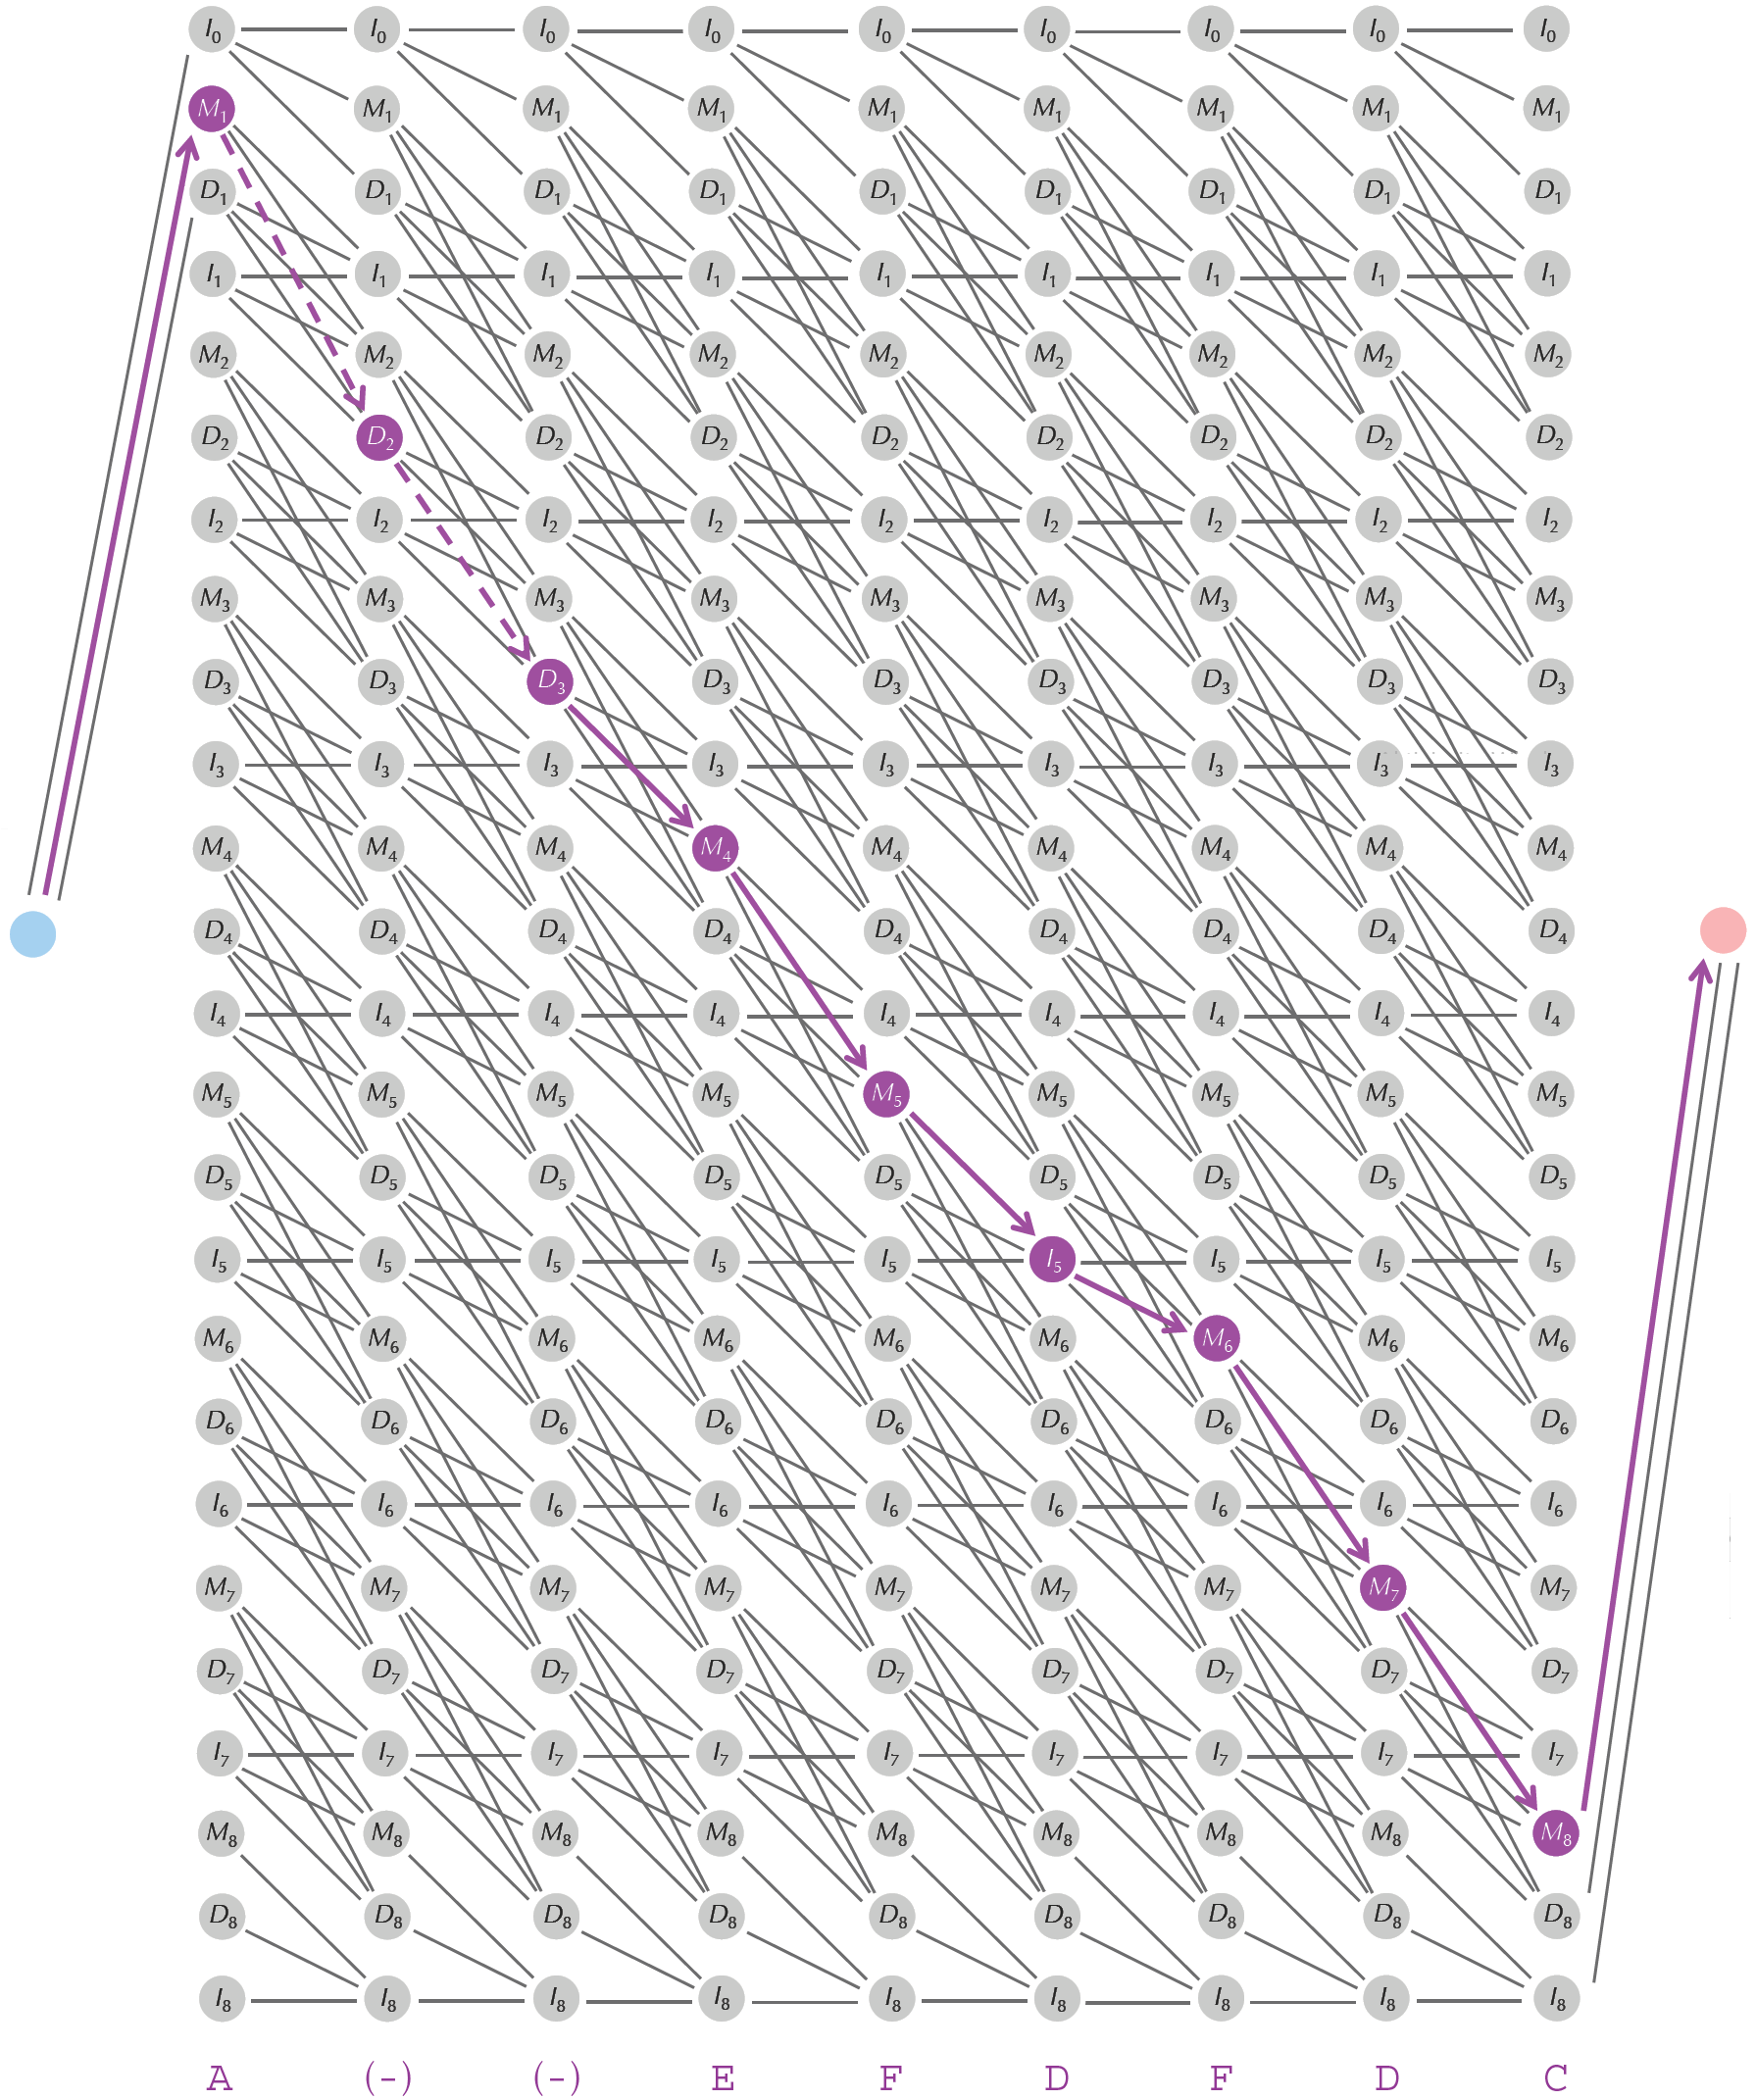
\includegraphics[width=\textwidth]{prof_vit.png}
  \caption{Наивни Витербијев граф профилног \textit{HMM} \cite{compeau2015}}
  \label{fig:prof_vit}
\end{figure}

Подсећања ради, основа Витербијевог графа је мрежа чворова чије редове чине сва могућа скривена стања (у конкретном случају профилног модела, за $n = 8$, има их $25$, без експлицитног почетног и завршног, а у општем $3n+1$), док колоне означавају ток времена, тренутак $t$. Из сваког чвора у колони $t-1$ усмерена је по једна грана у сваки чвор из колоне $t$, али искључиво ако је дозвољен прелаз између та два стања. Тако је на основу чињенице да се из сваког стања у тренутку $t-1$ може прећи у било које стање у тренутку $t$, уколико је вероватноћа преласка ненулта. Поред ове основе, мрежа има и два посебна чвора -- извор (експлицитно почетно стање -- плави кружић) и понор (експлицитно завршно стање -- црвени кружић). Из извора иду три гране -- ка $I_0$, $M_1$ и $D_1$ -- док у понор увиру такође само три гране -- од $M_8$, $D_8$ и $I_8$ (односно од индекса $n$ уместо $8$ у општем случају). Број колона (тренутака) заправо је дужина пута $k$, а замисао овакве мреже управо и јесте да истовремено моделује све скривене путеве дужине $k$ кроз упитни \textit{HMM}.

Проблем код графа са слике \ref{fig:prof_vit} управо је превише прецизно одабран број колона. Приказани граф као да зна да је оптимални пут дужине $k = 9$, а љубичасто опажање заправо $A--EFDFDC$ уместо $AEFDFDC$. Овакво знање, међутим, не може бити доступно пре покретања алгоритма, што значи да граф са слике \ref{fig:prof_vit} технички и није Витербијев. Штавише, могао би се направити већи број графова сличних претходном, али нпр. без друге и/или треће колоне, и потпуно једнако употребити за одређивање оптималног пута. Резултат, међутим, не би био тачан, јер би се разматрали само путеви дужине $k < 9$, па се свакако не би могао добити оптимални, чија је дужина $k = 9$.

Витербијев граф стога мора имати фиксан број колона, и то овде тачно $k = 7$. То је заправо број емитованих симбола, односно дужина познатог опажања, а не непознатог скривеног пута. Ово пре увођења стања делеције није било проблематично, пошто су дужина опажања и дужина оптималног скривеног пута увек биле једнаке. Тиха стања, међутим, нарушавају ову једнакост. У конкретном случају профилних \textit{HMM}, опажање дужине $k$ може настати на скривеном путу који је најмање дужине баш $k$, уколико пут садржи само стања поклапања, а највише $n+k$, уколико пут не садржи ниједно стање поклапања. Сада је циљ Витербијевим графом са $k$ колона некако моделовати путеве различитих дужина, а на којима се емитује тачно $k$ симбола.

Проблем, дакле, праве тиха стања делеције, пошто мењају смисао чвора $(x_i, t)$ графа. Првобитно, пролазак кроз тај чвор значио је да се у тренутку $t$ модел налази у стању $x_i$, односно да је симбол $o_t$ улазног опажања $o$ емитован из стања $x_i$. Ово, међутим, нема смисла код тихих стања, која ништа не приказују. Поправљени Витербијев граф приказан је на слици \ref{fig:prof_vit2}.

\begin{figure}[H]
  \centering
  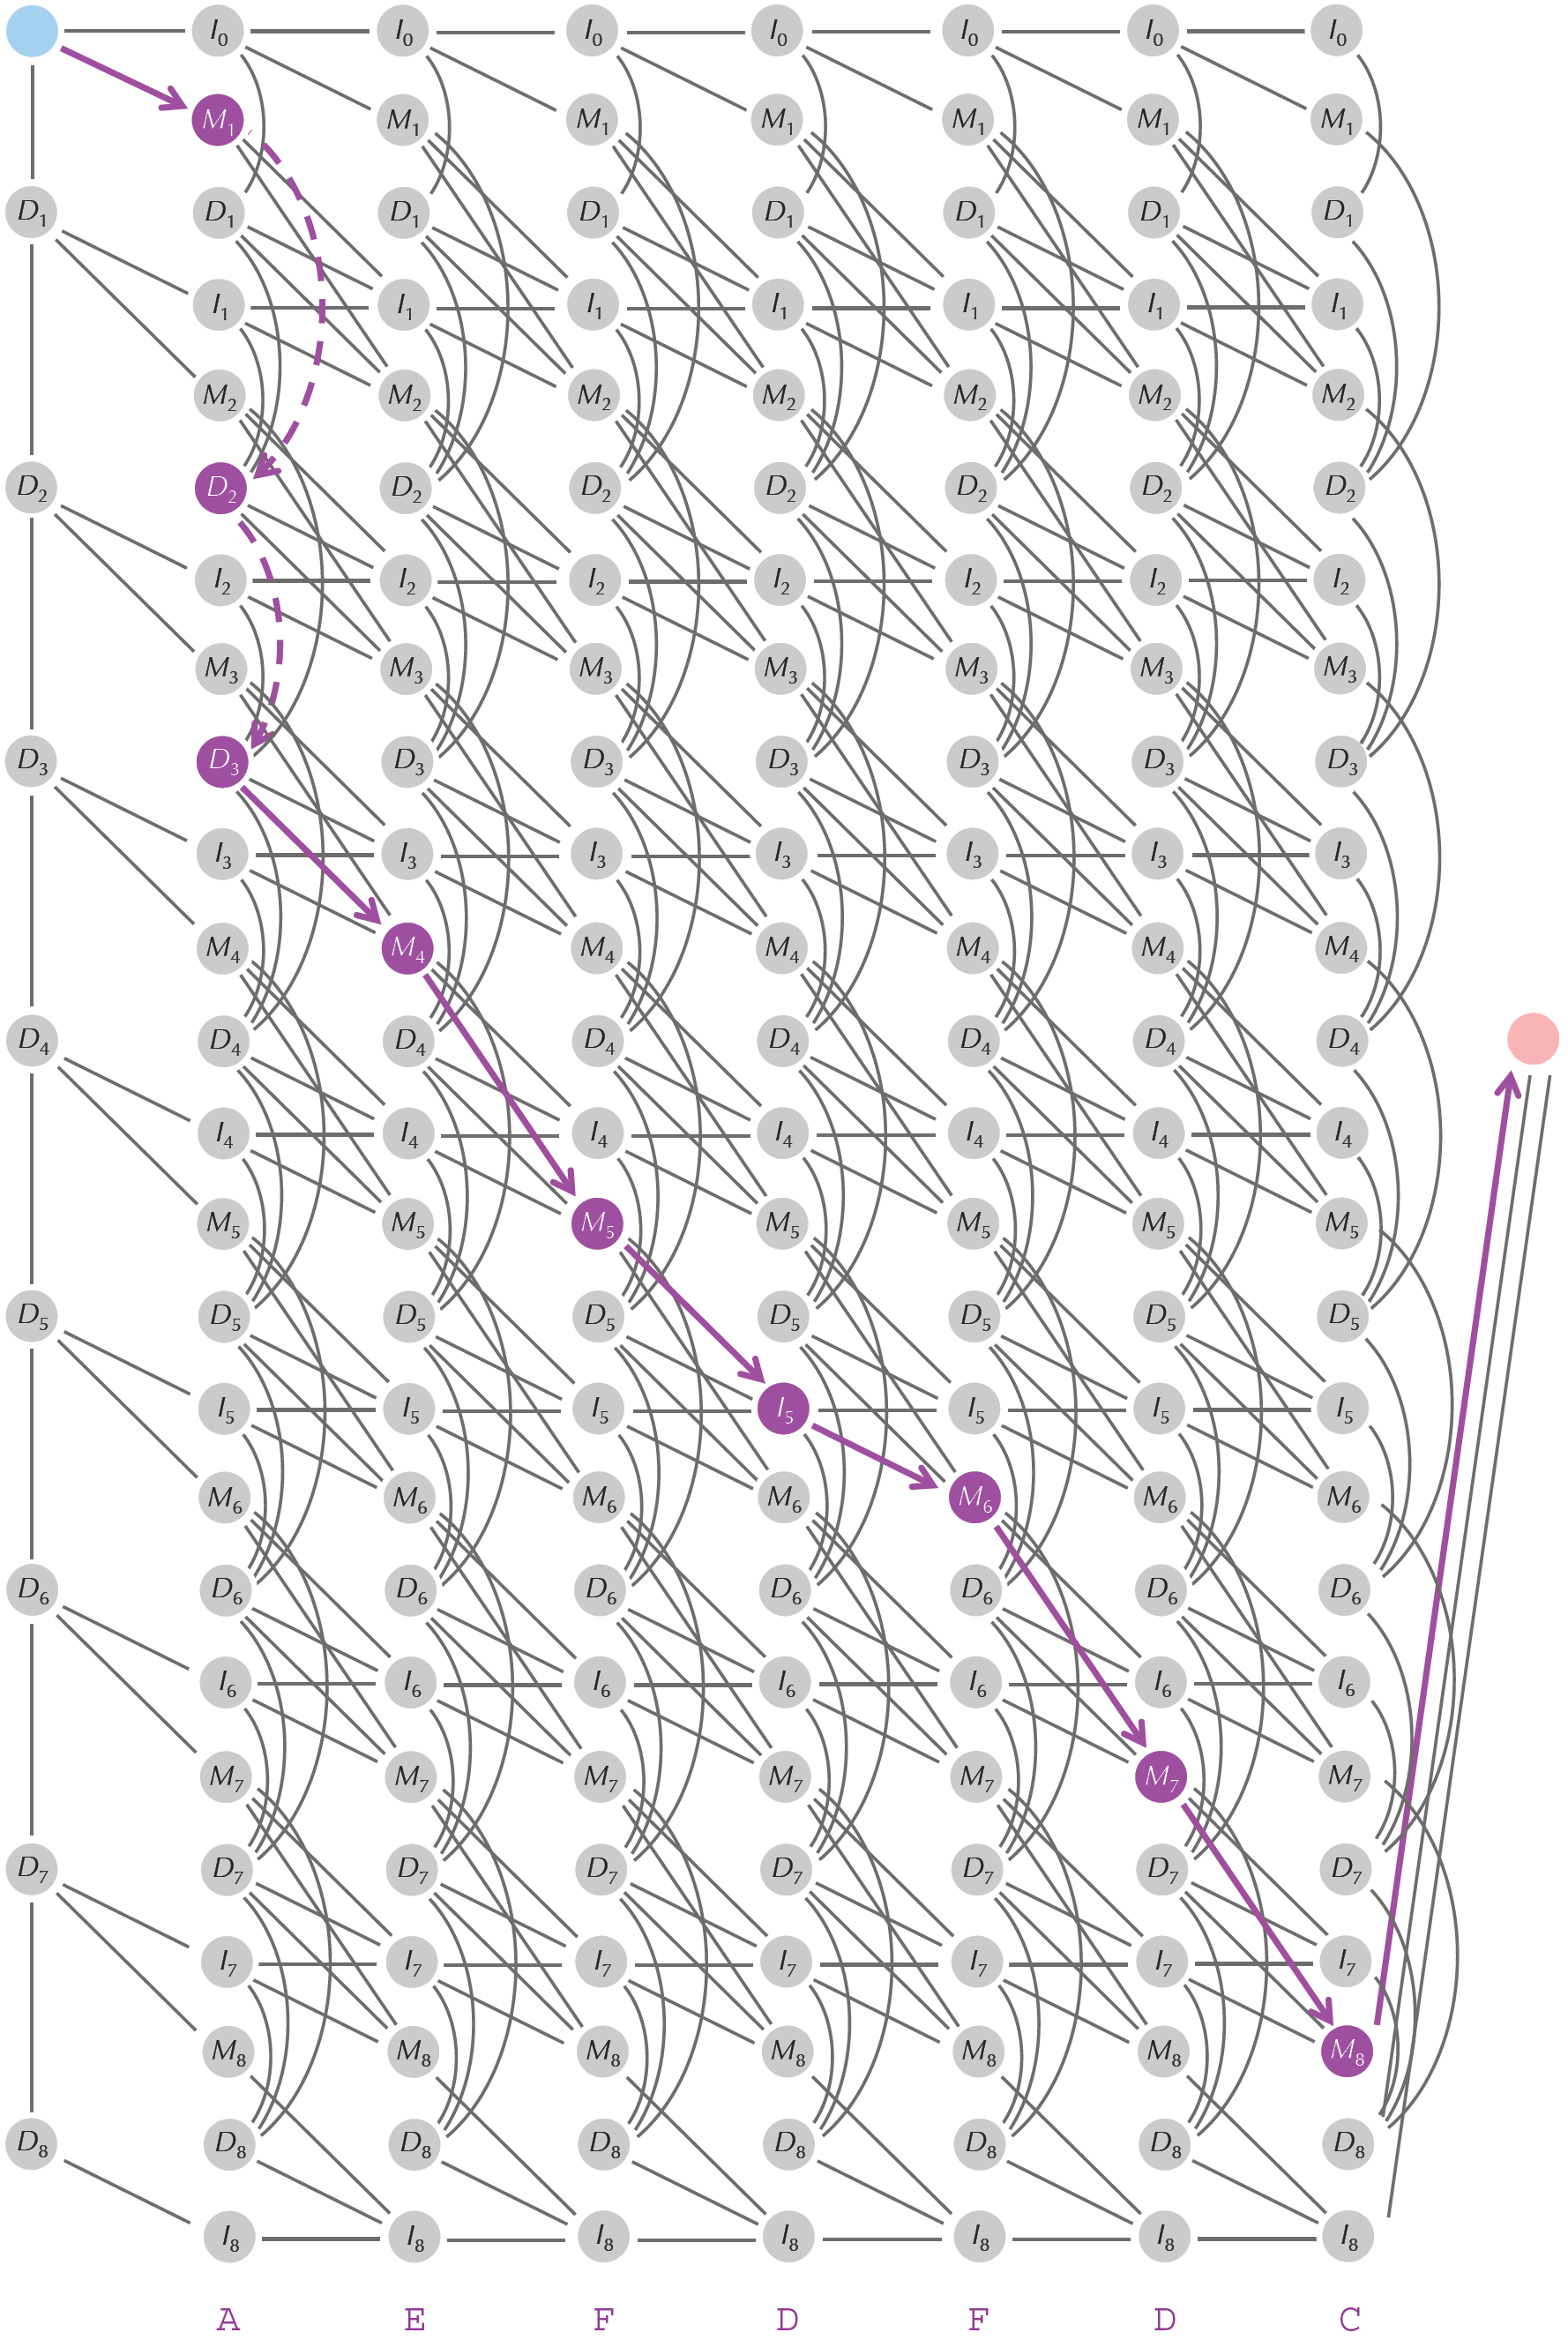
\includegraphics[width=.85\textwidth]{prof_vit2.png}
  \caption{Коначни Витербијев граф профилног \textit{HMM} \cite{compeau2015}}
  \label{fig:prof_vit2}
\end{figure}

Смисао се сада допуњује у следећи: пролазак кроз чвор $(x_i, t)$ графа значи да се \textit{HMM} налазио у стању $x_i$ када је емитовао симбол $o_t$ уколико стање $x_i$ није тихо, односно да се налазио у тихом стању $x_i$ након емитовања симбола $o_t$, а пре емитовања $o_{t+1}$. У конкретном случају профилних модела, пролазак кроз $(M_i, t)$ или $(I_i, t)$ значи да је у стању поклапања $M_i$ или инсерције $I_i$ емитовано $o_t$, док пролазак кроз $(D_i, t)$ означава да је аутомат био у тихом стању делеције $D_i$ између емитовања суседних симбола опажања $o_t$ и $o_{t+1}$.

У коначној верзији Витербијевог графа са слике \ref{fig:prof_vit2}, претходно објашњена допуна смисла очитава се двама променама. Прво, сваки прелаз у стање делеције, дакле прелаз облика $I_i \mapsto D_{i+1}$, $M_i \mapsto D_{i+1}$ или $D_i \mapsto D_{i+1}$, сада се дешава у оквиру исте колоне. Ово непосредно осликава чињеницу да делеција не емитује нови симбол, што значи да индекс (тренутак) $t$ остаје непромењен. Наравно, преласци ка стањима поклапања или инсерције остају скок у следећу колону, пошто за собом повлаче нову емисију. Ово значи да једна колона строго одговара опажању једног симбола, мада се то може десити проласком кроз различите скривене путеве, што је и био циљ.

Друга промена одговара проширењу нулте колоне, у којој се досад налазио само извор. Она се проширује низом (ланцем) повезаних стања делеције, свим могућим од $D_1$ до $D_8$, односно $D_n$ у општем случају. Наиме, уколико не би било тог проширења, пут би завршио у ћорсокаку уколико би започео првим стањем делеције $D_1$ у првој колони. Прелази су једноставно такви да након уласка у стање делеције није више могуће емитовати симбол у текућој колони. Стога се тај прелаз пребацује у нулту колону, сачињену искључиво од тихих стања. Подразумевано, све гране у истој колони оријентисане су надоле, док су прелази између колона оријентисани надесно. И слика \ref{fig:prof_vit2}, попут претходне, декодира љубичасту ниску $AEFDFDC$ из уводног поравнања.

Поравнање помоћу профилног \textit{HMM}-а формално се дефинише кроз проблем \ref{prob:poravnanje}. Реч је, дакле, о нешто напреднијем декодирању, дорађеној верзији проблема \ref{prob:dekod}. Решење оба је Витербијев алгоритам, само се разликује Витербијев граф над којим се ради, пошто сад постоје и тиха стања делеције.

\begin{problem}[H]
  \SetAlgoLined
  \textit{Поравнати нову ниску са фамилијом -- профилни \textit{HMM}.}\\
  \textbf{Улаз}: вишеструко поравнање $P$, граница одсецања $\theta$, псеудовредност $\sigma$, нова ниска (опажање) $o$.\\
  \textbf{Излаз}: оптимални пут $p$ кроз $HMM(P, \theta, \sigma)$ за ниску $o$.
  \caption{Поравнање са профилним моделом \cite{ba10g}}
  \label{prob:poravnanje}
\end{problem}

На сличан начин је, иначе, могуће конструисати Витербијев граф за произвољни \textit{HMM} са тихим стањима. Једини услов који мора да буде испуњен јесте да не постоје петље или циклуси који се састоје искључиво од тихих стања. У супротном, није могуће решити проблем декодирања, али ни друге сличне проблеме засноване на Витербијевом графу (алгоритам "напред" итд.).

Ово је аналогно чињеници да није могуће решити проблем оптималног обиласка Менхетн графа са циклусима. Разлог томе је што се, како код Менхетн, тако и код Витербијевог графа, вредности морају рачунати према тополошком редоследу чворова. Другим речима, неопходно је да буду познате све родитељске вредности како би се евалуирао нови, текући чвор.

\begin{figure}[H]
  \centering
  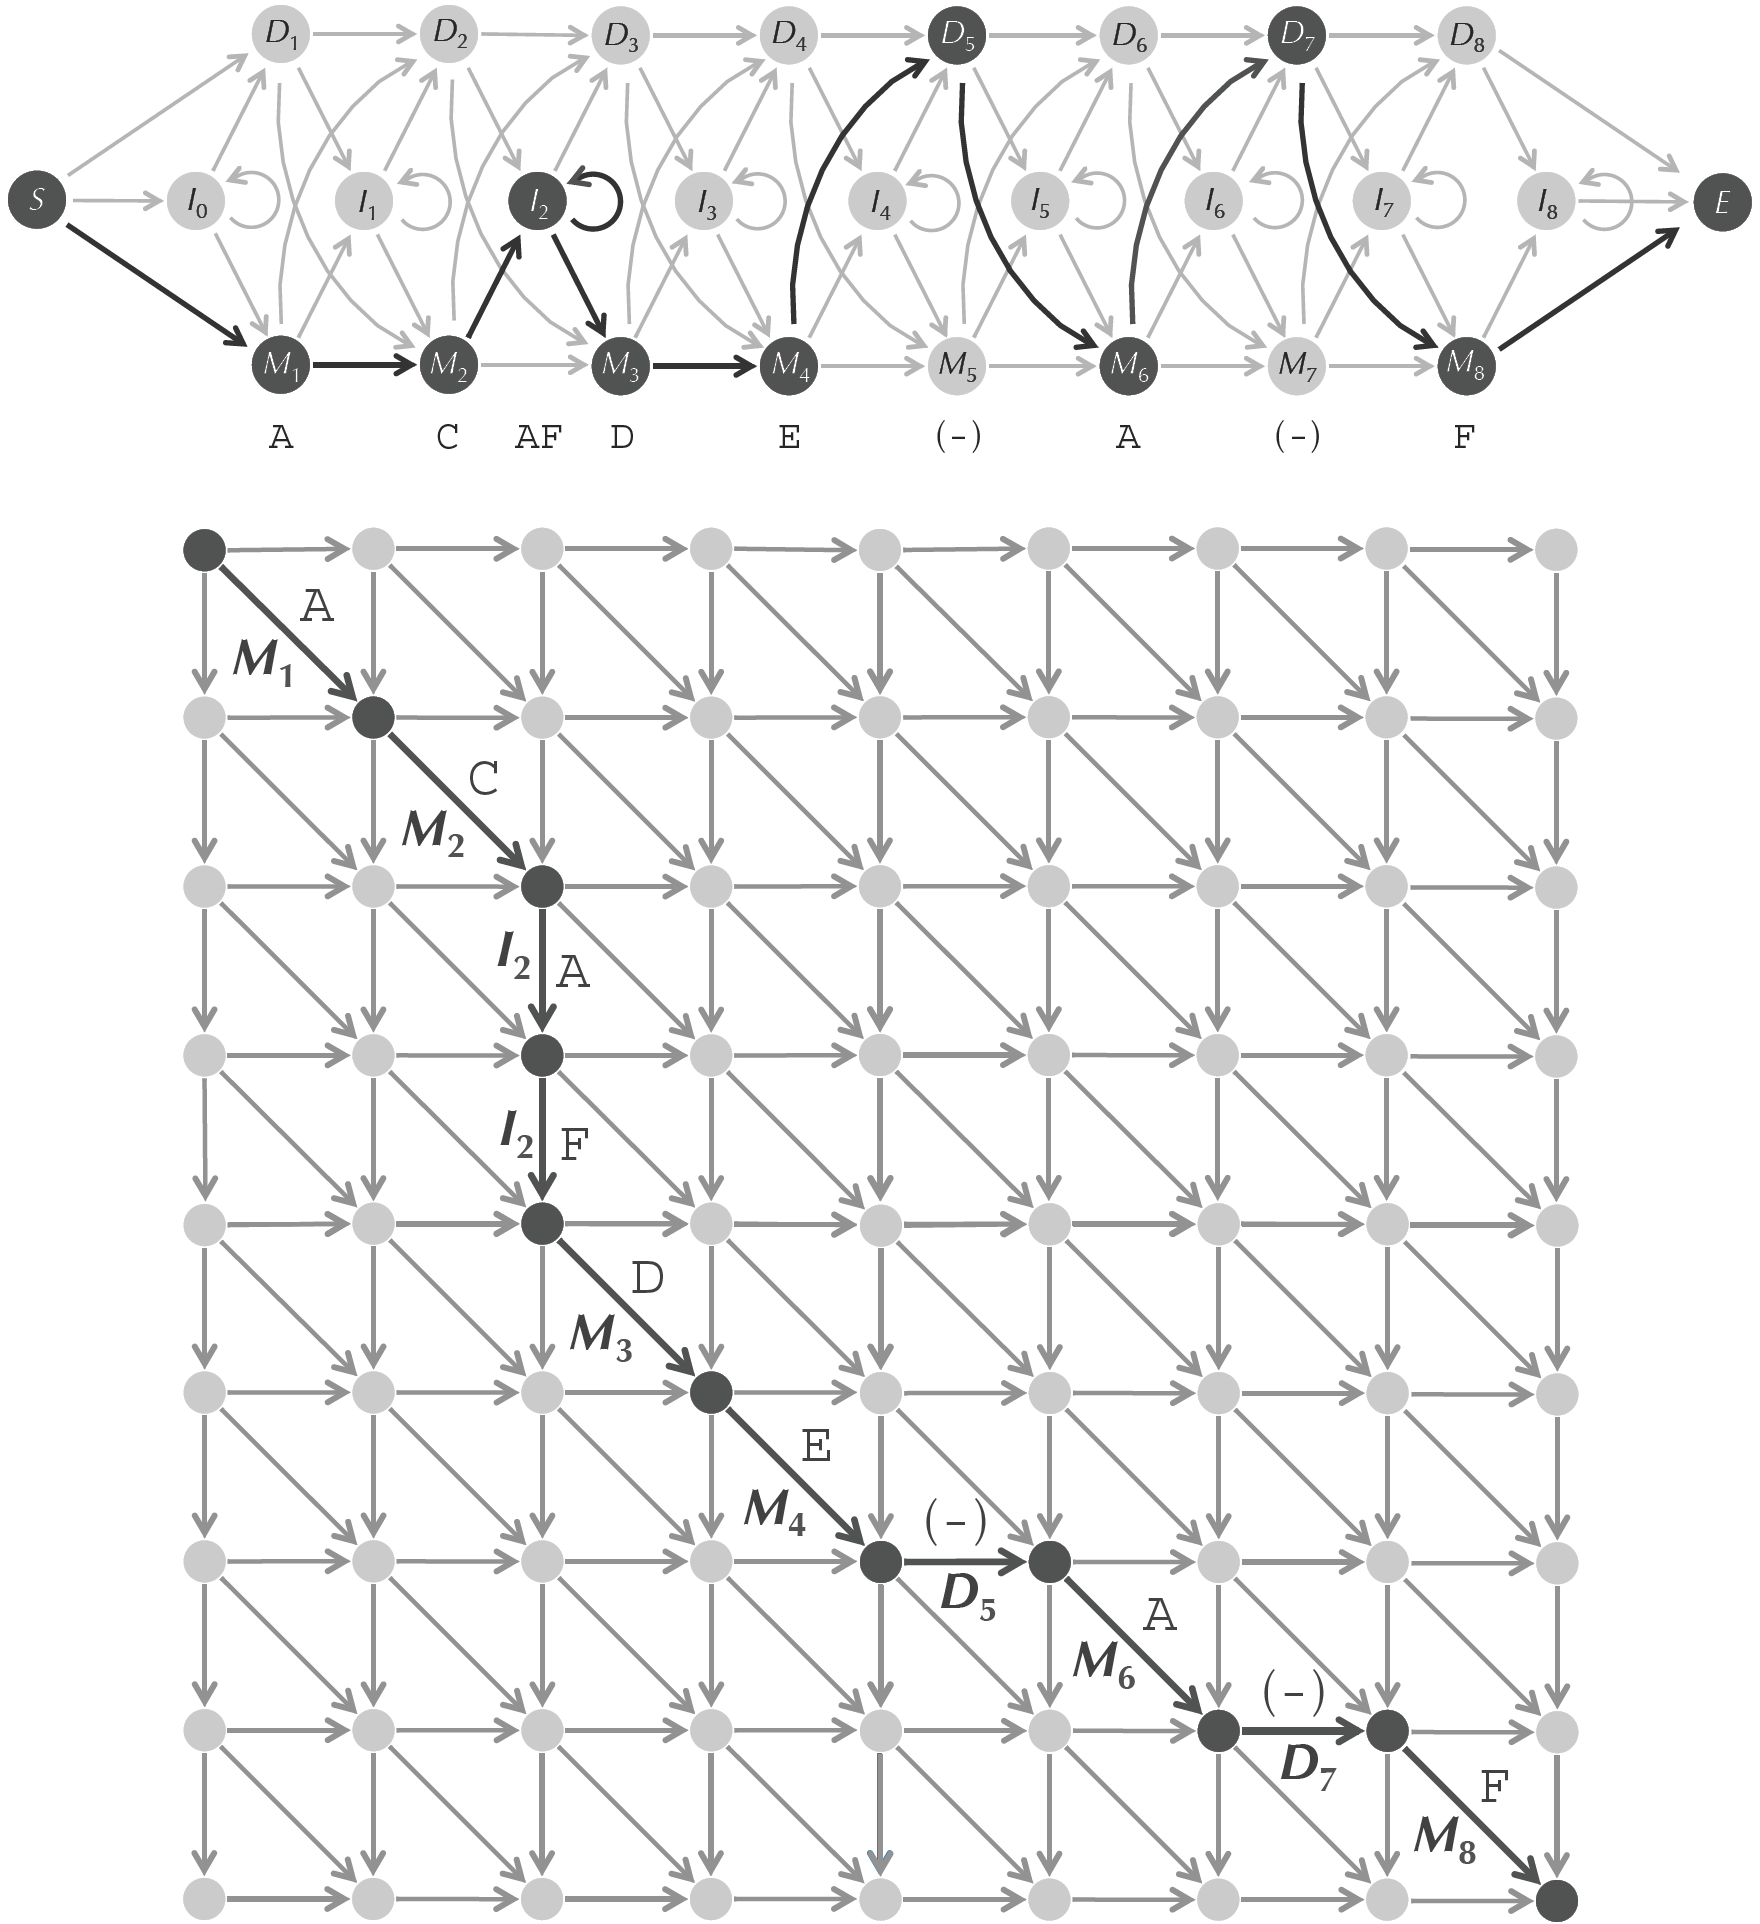
\includegraphics[width=.85\textwidth]{poravnanje2.png}
  \caption{Поређење поравнања мотивационог примера \cite{compeau2015}}
  \label{fig:poravnanje2}
\end{figure}

Граф, дакле, мора бити без циклуса -- усмерени ациклички граф. Тополошки редослед у супротном не постоји. У конкретном случају профилних \textit{HMM}, уобичајен редослед рачунања је слева надесно, од врха надоле. Успут се, наравно, чувају путокази, како би се оптимални пут на крају могао реконструисати. Без њих, добила би се само вероватноћа најбољег пута.

Сличност између Витербијевог и Менхетн графа није случајна. Испоставља се да нису само аналогни проблеми, већ и структуре. На слици \ref{fig:poravnanje2} приказана је њихова наизглед једнакост на познатом примеру ниске $ACAFDEAF$ и њеног поравнања са слике \ref{fig:poravnanje}. Слика илуструје како пут у Менхетн графу одговара скривеном путу кроз профилни \textit{HMM}. Дијагоналне ивице Менхетн графа одговарају поклапањима, усправне инсерцијама, а водоравне делецијама. Важно је истаћи да ова аналогија ипак није једнакост (еквиваленција), пошто код \textit{HMM}-а постоје променљиве вероватноће (тежине) прелаза и емисија, што није могуће моделовати помоћу Менхетн графа.

Способност профилних скривених Марковљевих модела да различито оцењују различите колоне матрице поравнања издваја их као прецизније у односу на једноставне методе поравнања засноване на једној матрици са истим скоровима. Профилни модели тако могу ухватити суптилне сличности, које једноставна поравнања пропуштају. Упркос тој предности, сложеност остаје подједнако добра, и износи $O(nk)$ за $n$ колона (дужина полазног поравнања) и $k$ редова (дужина опажања).

Код Менхетн графа је сложеност очигледна, јер се оперише над матрицом димензија $n \times k$, где се вредност сваког чвора израчунава кроз највише три гране. Ни код профилних \textit{HMM} није тешко одредити је. Већ је више пута напоменуто да је сложеност Витербијевог алгоритма сразмерна броју грана у Витербијевом графу. У општем случају, када се из сваког стања може прећи у било које друго, износи $O(n^2 k)$, што је последица постојања по $n$ прелаза између $n$ стања у $k-1$ промени тренутка. Код профилних \textit{HMM}, међутим, постоји већи број стања $3n+1$, као и већи број промена тренутка $k$, али је прелаза највише по три (константа), тако да је асиптотски производ $O(nk)$.

За крај, следе тачне формуле максимизације вероватноће пута у чворовима Витербијевог графа код профилних \textit{HMM} са $n$ колона поравнања за познато опажање $o$ дужине $k$. Још једном, нека мапа скорова $s$ буде таква да $s_{x_i, t}$ складишти вероватноћу оптималног пута дужине $t$ који се завршава скривеним стањем $x_i$. У конкретном случају, уместо општих стања $x_i$, одвојено се разматрају специјализована стања поклапања $M_i$, делеције $D_i$ и инсерције $I_i$.

База рекурзије овако постављеног проблема јесте (први чланови низа): $$\dvareda{$(i = 1)$\\$(t = 1)$} s_{M_1, 1} = a_{S, M_1} \cdot b_{M_1, o_1},$$ $$\dvareda{$(i = 1)$\\$(t = 0)$} s_{D_1, 0} = a_{S, D_1},$$ $$\dvareda{$(i = 0)$\\$(t = 1)$} s_{I_0, 1} = a_{S, I_0} \cdot b_{I_0, o_1}.$$ Рекурзивне формуле максимизације су (непостојећи индекси се занемарују, а ради краћег записа уводи се помоћни скуп типова стања $X = \{M, D, I\}$): $$\dvareda{$(\forall i \in \{2, ..., n\})$\\$(\forall t \in \{2, ..., k\})$} s_{M_i, t} = \max_X \{s_{X_{i-1}, t-1} \cdot a_{X_{i-1}, M_i} \cdot b_{M_i, o_t}\},$$ $$\dvareda{$(\forall i \in \{2, ..., n\})$\\$(\forall t \in \{1, ..., k\})$} s_{D_i, t} = \max_X \{s_{X_{i-1}, t} \cdot a_{X_{i-1}, D_i}\},$$ $$\dvareda{$(\forall i \in \{1, ..., n\})$\\$(\forall t \in \{2, ..., k\})$} s_{I_i, t} = \max_X \{s_{X_i, t-1} \cdot a_{X_i, I_i} \cdot b_{I_i, o_t}\}.$$ Коначан оптимални (највероватнији) пут добија се додатном максимизацијом: $$P\{p_{opt}, o\} = \max_p P\{p, o\} = \dvareda{$(i = n)$\\$(t = k)$} \max_X \{s_{X_n, k} \cdot a_{X_n, E}\}.$$

Као и досад, аналогно се формирају логаритамске верзије формула, које множење мењају сабирањем, чиме се смањује грешка у рачуну, а проблем додатно приближава Менхетн графу. Идентична је и општа верзија формула са произвољним тежинама $\tau$. Поред декодирања као проблема \ref{prob:poravnanje}, једнако се приступа и осталим задацима заснованим на Витербијевом графу -- табела \ref{tab:hmm}. Решење је такође у одабиру одговарајућих оператора уместо максимума.

% ------------------------------------------------------------------------------
\chapter{Учење модела}
% ------------------------------------------------------------------------------
У претходним главама је приказана употреба скривених Марковљевих модела у решавању биолошких проблема који се могу схватити како као задаци надгледаног (класификација протеина), тако и ненадгледаног машинског учења (означавање \textit{CG} острва). У овој се излагање допуњује још једном важном особином \textit{HMM} у вези са машинским учењем -- способност учења поткрепљивањем. Претходно је било речи о готовим моделима, али прави потенцијал \textit{HMM} показују тек када се сви параметри модела науче. Успут је предочен и један нов и кориснији поглед на већ познати проблем декодирања.

% Learning the Parameters of an HMM
\section{Витербијево учење}
У оквиру одређивања профилних \textit{HMM} на основу улазног вишеструког поравнања, представљена је хеуристика за процену њихових параметара -- мапа вероватноћа прелаза и емисија. Подсећања ради, идеја се састоји из следећих корака: свака ниска из поравнања сматра се једним опажањем (све ниске чине узорак), на основу поравнања непосредно и једнозначно се одређује позадински скривени пут, прелази и емисије симбола пребројавају се проласком кроз претходно одређене путеве, а на крају се број појављивања нормализује у удео, који је управо претпостављена вероватноћа према улазном узорку.

Поставља се питање да ли је овај једноставни приступ могуће уопштити на произвољан \textit{HMM}. Одговор је у општем случају одричан, пошто није могуће на основу опажања непосредно одредити скривени пут на коме је оно настало. Могуће је одредити највероватнији такав пут, али једино ако су параметри већ познати, што код овог проблема није случај. Одговор је, међутим, потврдан уколико је уз опажање познат позадински пут. Тада је довољно приступити пребројавању и одређивању удела, као код \textit{HMM} профила. Овакво надгледано учење параметара модела формално се представља проблемом \ref{prob:params}.

\begin{problem}[H]
  \SetAlgoLined
  \textit{Наћи оптималне параметре \textit{HMM}-а према обележеном узорку.}\\
  \textbf{Улаз}: скривени пут $p = p_1...p_k$ кроз \textit{HMM} са непознатим параметрима и ниска $o = o_1...o_k$ емитована на том путу.\\
  \textbf{Излаз}: оптимални параметри, који максимизују $P\{p, o\}$.
  \caption{Надгледано учење параметара \cite{ba10h}}
  \label{prob:params}
\end{problem}

Мада се испоставља да учење из обележеног узорка даје глобално оптималне параметре -- такве да максимизују заједничку вероватноћу улазног исхода и пута на ком је настао, овај приступ често није применљив. Скривена стања су по правилу стварно скривена, те нису доступни парови опажања и путева, већ само опсервације. Стога је следећи задатак нешто амбициознији -- одредити параметре само на основу опажања, према проблему \ref{prob:vituch}.

\begin{problem}[H]
  \SetAlgoLined
  \textit{Наћи оптималне параметре \textit{HMM}-а према узорку опажања.}\\
  \textbf{Улаз}: ниска $o = o_1...o_k$ и \textit{HMM} са непознатим параметрима који ју је емитовао проласком кроз такође непознати пут $p = p_1...p_k$.\\
  \textbf{Излаз}: оптимални параметри, који максимизују $P\{p, o\}$.
  \caption{Ненадгледано учење параметара \cite{ba10k, ba10i}}
  \label{prob:vituch}
\end{problem}

На примеру непоштеног казина, проблем \ref{prob:params} односио се на одређивање пристрасности (вероватноће главе) непоштеног новчића ако је јаван податак када га крупије баца. Како крупије то вешто крије, сада је решењем општијег проблема \ref{prob:vituch} циљ доћи до тог податка само на основу увек познатог низа исхода -- у ком бацању је пала глава, а у ком писмо.

Добри резултати могу се добити итеративном хеуристиком попут оне која је основа Лојдовог алгоритма. Реч је о алгоритму који решава проблем кластеровања $k$-средина. У случају скривених Марковљевих модела, параметри $P$ случајно се иницијализују, чиме се за почетак добијају насумичне вероватноће. Затим се улазна ниска $o$ декодира (проблем \ref{prob:dekod}), чиме се добија скривени пут $p$ по принципу $(o, ?, P) \mapsto p$. Потом се израчунавају нови параметри (проблем \ref{prob:params}), по принципу $(o, p, ?) \mapsto P$, и тако наизменично. Ово је уобичајени алгоритам максимизације очекивања (\textit{EM[A]}, према енгл. \textit{expectation-maximization [algorithm]}), који се илуструје дијаграмом са слике \ref{fig:ema}.

\begin{figure}[H]
  \centering
  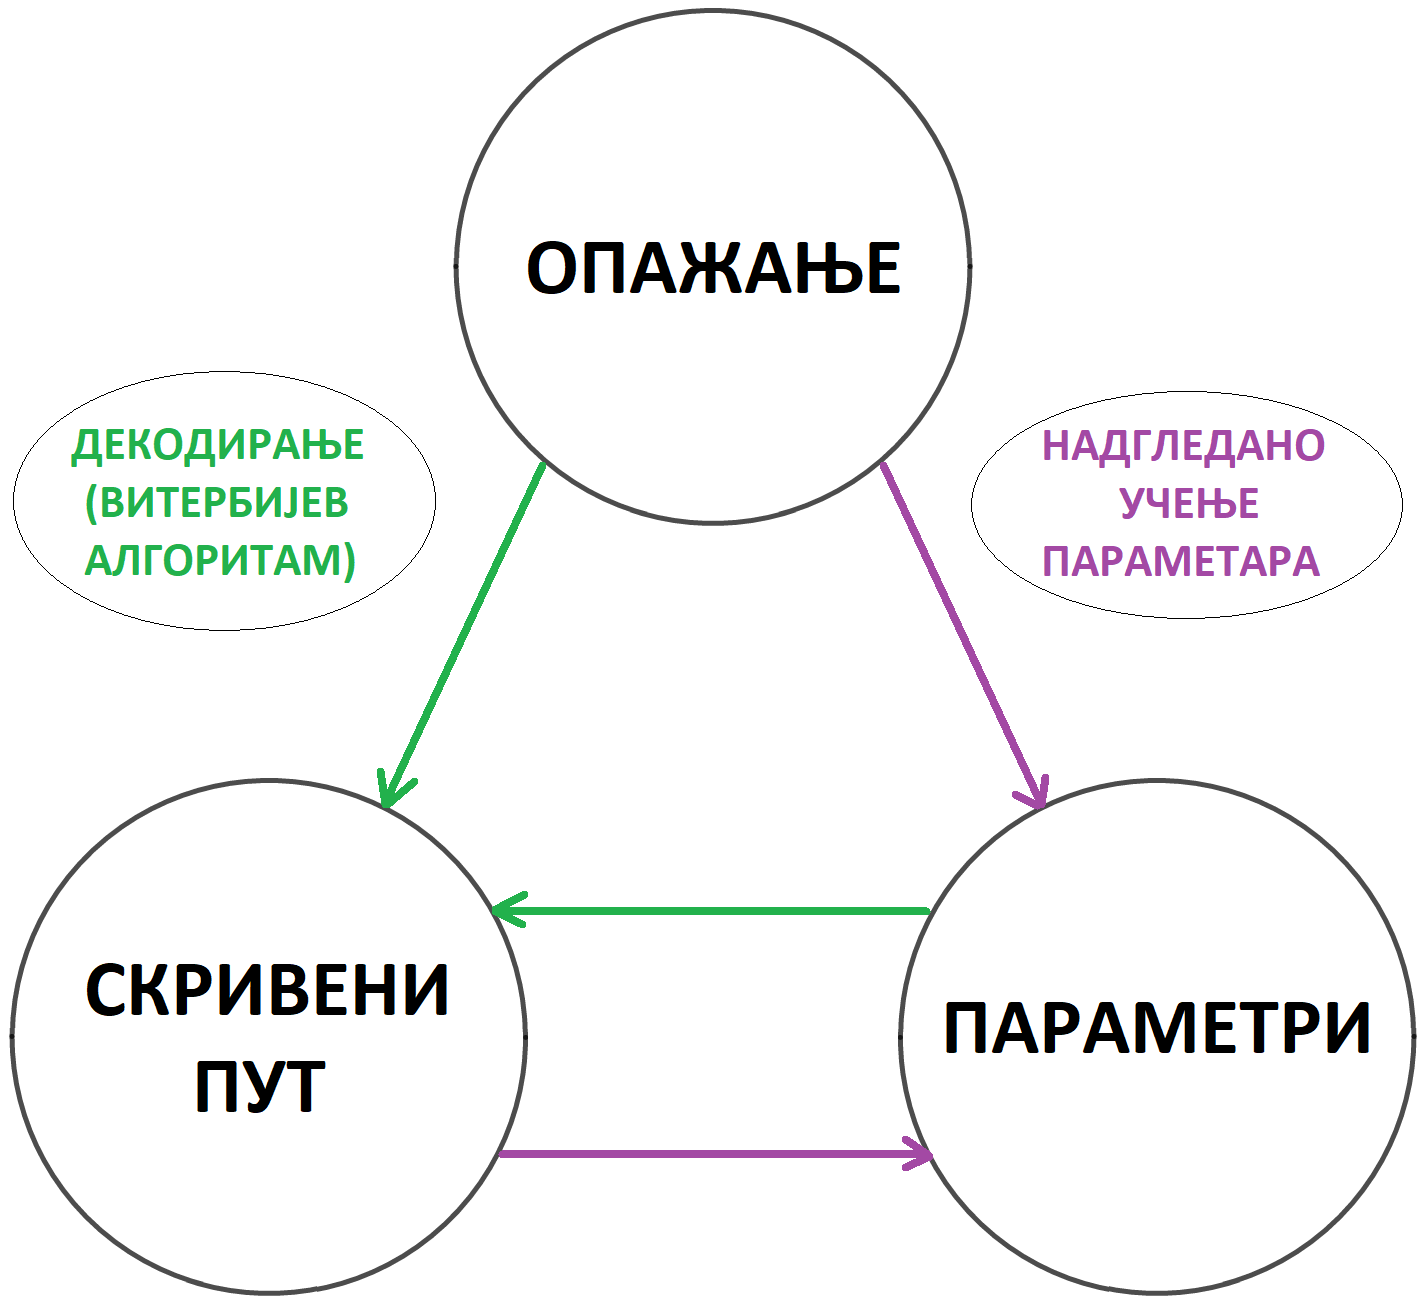
\includegraphics[width=.65\textwidth]{ema.png}
  \caption{Максимизација очекивања код \textit{HMM}}
  \label{fig:ema}
\end{figure}

Овакав ненадгледани приступ учењу параметара модела назива се Витербијевим учењем, пошто му је у основи Витербијев алгоритам за декодирање. Тај део алгоритма представља корак очекивања (\textit{\textcolor{green}{E}} корак), док је надгледано одређивање параметара које следи корак максимизације (\textit{\textcolor{violet}{M}} корак). Дубљом анализом, испоставља се да је ненадгледана оптимизација параметара \textit{HMM}-а тежак проблем, тако да је Витербијево учење сасвим задовољавајућа хеуристика. Најважнија особина му је то што је вредност $\max_p P\{p, o\}$ за улазно опажање $o$ због природе \textit{EM} алгоритма током оптимизације монотоно неопадајућа. То значи да су сваком итерацијом параметри ближи најбољим.

Наравно, како је и иначе случај код хеуристичких приступа, није необично заглављивање алгоритма у локалном максимуму, тако да резултат умногоме зависи од почетних вредности параметара. Како су оне случајне, уобичајена тактика за добијање бољих резултата јесте покретање алгоритма учења већи број пута, а затим узимање најбољих параметара из свих покретања. Што се тиче критеријума заустављања, најчешћа су два: унапред одређени број итерација или граница минималног повећања вероватноће која се максимизује.

Поред случајне иницијализације параметара на почетку алгоритма, могуће је кренути од неких унапред одређених, односно познатих параметара. У том случају циљ није (само) ненадгледано их научити, већ профинити претходне. Тада је Витербијево учење прави пример учења поткрепљивањем, јер се параметри прилагођавају новим околностима на основу нових опажања.

Уколико је критеријум број итерација, у овој верзији их је обично мање, јер у супротном долази до добијања екстремних вредности, што се може протумачити као преприлагођавање модела. На примеру непоштене коцкарнице, већи број итерација код поткрепљивања доводи до закључка да је вероватноћа пада главе код пристрасног новичића јединична, а писма нулта. Овакво понашање, с друге стране, може бити пожељно баш због способности откривања екстремних вредности. У случају коцкарнице, након поткрепљивања нема сумње да је пристрасни новчић управо онај са јединичном вероватноћом главе, иако је пристрасност на почетку можда била релативно мала.

Познату примену \textit{HMM} овог типа у лингвистици осмислили су 1980. године Кејв и Нојвирт \cite{cave1980}, док су је други аутори касније проширили \cite{stamp2021}. Илустративна претпоставка је да научник Марсовац жели да сазна нешто о писаном језику Земљана. За те потребе набавио је велику количину текста, на пример корпус енглеског језика. Пало му је на памет да покуша да слова језика подели на статистички значајно различите скупове, што моделује управо помоћу скривених Марковљевих модела, за које је стручњак. Како је реч о енглеском језику, могућих симбола је двадесетак, за свако слово по један (код осталих језика би их било више или мање), а Марсовац је одабрао да постоје само два скривена стања, како би модел остао једноставан. Параметре модела је случајно (скоро равномерно) иницијализовао, а затим је покренуо ненадгледано поткрепљивање, користећи текст корпуса као улазно опажање.

Резултујућа мапа емисија прилично је занимљива -- испоставља се да је сваки самогласник скоро сигурно опажен у једном стању, а сугласник у другом. Овиме је, дакле, Марсовац добио практично савршену поделу (груписање -- кластеровање) симбола о којима ништа не зна на вокале и консонантне, што без проблема може да закључи на основу добијених екстремних вероватноћа емисија. Још неки занимљиви резултати могу се добити употребом већег броја стања, посебно дванаест, о чему се детаљније може прочитати у цитираном раду. На сличан начин функционише и решавање других проблема ненадгледаног учења помоћу \textit{HMM}, мада се чешће уместо Витербијевог користи моћније Баум-Велчово учење, о коме ће бити речи у наставку.

% Soft Decisions in Parameter Estimation
% Baum-Welch Learning
\section{Баум-Велчово учење}
У тексту посвећеном општем опису скривених Марковљевих модела, било је речи о одређивању вероватноће опажања дужине $k$, кроз проблем \ref{prob:ops}. Као решење, изложен је алгоритам "напред", заснован на мапи $f$ (од енгл. \textit{forward}), чији елемент $f_{x_i, t}$ складишти вероватноћу префикса опажања дужине $t$ (подниз $o_1...o_t$), насталог на скривеном путу који завршава стањем $x_i$.

Аналогно се формира обрнута мапа $w$ (од енгл. \textit{backward}), чији елемент $w_{x_i, t}$ складишти вероватноћу суфикса опажања дужине $k-t+1$ (подниз $o_t...o_k$), насталог на скривеном путу који започиње стањем $x_i$. Мапа такође садржи вероватноћу целог опажања, а попуњава се на исти начин као претходна, праћењем Витербијевог графа, само обрнутим редоследом. Овакав приступ назива се алгоритам "назад" и код њега важе следеће рекурентне формуле: $$w_{x_i, k} = 1,$$ $$w_{x_i, t} = \sum_j  a_{x_i, x_j} \cdot b_{x_j, o_{t+1}} \cdot w_{x_j, t+1},$$ $$P\{o\} = \sum_j \pi_{x_j} \cdot b_{x_j, o_1} \cdot w_{x_j, 1}.$$ Још једном, аналогно се изводе логаритамске верзије претходних формула.

Спајањем алгоритма "напред" и "назад", добија се нов и кориснији поглед на проблем декодирања. Наиме, сваки пут кроз Витербијев граф може се пресећи у неком чвору и тако поделити на два дела. Како то изгледа на примеру пута $FFF$ у непоштеној коцкарници, пресеченог у средњем чвору, дато је на слици \ref{fig:tripod}. Префикс је наглашен црвеном, а суфикс плавом бојом.

\begin{figure}[H]
  \centering
  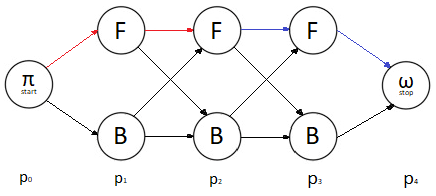
\includegraphics[width=.9\textwidth]{tri_podela.png}
  \caption{Подела пута кроз граф са три бацања}
  \label{fig:tripod}
\end{figure}

Вероватноћа црвеног префикса дужине $t$ са пресеком у стању $x_i$ може се израчунати алгоритмом "напред" као вредност $\textcolor{red}{f_{x_i, t}}$ из мапе, док се вероватноћа одговарајућег плавог суфикса израчунава као $\textcolor{blue}{w_{x_i, t}}$ из алгоритма "назад". Како вредност из мапе $f$ покрива све могуће префиксе, а вредност из $w$ све суфиксе, они заједно покривају све могуће путеве који у тренутку $t$ пролазе кроз стање $x_i$. Стога је њихов производ заправо заједничка вероватноћа да је \textit{HMM} емитовао ниску $o$, при чему је у тренутку $t$ био баш у стању $x_i$: $$P\{p_t = x_i, o\} = \textcolor{red}{f_{x_i, t}} \cdot \textcolor{blue}{w_{x_i, t}}.$$

Оваква комбинација назива се алгоритам "напред-назад" и њен значај огледа се управо у томе што даје вероватносни резултат за све тренутке и сва стања. Претходно је моделована заједничка вероватноћа $P\{p, o\}$, чијом се максимизацијом Витербијевим алгоритмом добија један конкретан цео највероватнији пут. Добија се, дакле, "чврсто" решење проблема декодирања, према коме је \textit{HMM} у неком тренутку био у тачно одређеном стању.

Нови приступ, с друге стране, даје нов поглед на проблем утолико што сваком стању додељује по вероватноћу у сваком тренутку. Ово је аналогно "меком" кластеровању, које је надградња Лојдовог алгоритма, па се назива и "меким" декодирањем. Задатак се формално представља проблемом \ref{prob:meko}.

\begin{problem}[H]
  \SetAlgoLined
  \textit{Одредити вероватноћу да је \textit{HMM} у неком тренутку био у неком скривеном стању, ако је познато опажање.}\\
  \textbf{Улаз}: ниска $o = o_1...o_k$ и \textit{HMM}$\{a, b, \pi\}$ који ју је емитовао.\\
  \textbf{Излаз}: условна вероватноћа стања у тренутку $P\{p_t = x_i | o\}$.
  \caption{"Меко" декодирање приказа \cite{ba10j}}
  \label{prob:meko}
\end{problem}

Резултат оваквог декодирања није пут дужине $k$, већ низ $k$ расподела стања. Расподеле се нормализују, како би се добила условна вероватноћа: $$P\{p_t = x_i | o\} = \frac{P\{p_t = x_i, o\}}{P\{o\}} = \frac{\textcolor{red}{f_{x_i, t}} \cdot \textcolor{blue}{w_{x_i, t}}}{\textcolor{red}{\sum_j f_{x_j, k}}} = \frac{\textcolor{red}{f_{x_i, t}} \cdot \textcolor{blue}{w_{x_i, t}}}{\textcolor{blue}{\sum_j \pi_{x_j} \cdot b_{x_j, o_1} \cdot w_{x_j, 1}}}.$$ Посебно је занимљиво истаћи да стање $p_t$ добијено Витербијевим алгоритмом није нужно једнако стању $p_t$ максималне вероватноће према алгоритму "напред-назад". Стога постоји и "чврста" верзија "меког" декодирања, која у сваком тренутку одабира највероватније $p_t$. Она се назива апостериорним (\textit{MAP}, према енгл. \textit{maximum a posteriori}) декодирањем и може дати боље резултате од Витербија. Поређење приступа на примеру \textit{HMM} за проналажење \textit{CG} острва дато је у коду електронске лекције, где су наглашене разлике.

Поред пресецања графа у неком чвору, чиме се добија условна вероватноћа $P\{p_t = x_i | o\}$, могуће је фиксирати произвољни потпут и израчунати његову вероватноћу помоћу алгоритма "напред-назад". Наиме, довољно је помножити вероватноће одговарајућег префикса, суфикса и тежине грана фиксираног потпута. Посебно је значајно када је фиксирана једна грана, што је условна расподела $P\{p_t = x_i, p_{t+1} = x_j | o\}$. У том случају, тражи се вероватноћа да је, емитујући ниску $o$, упитни \textit{HMM} у тренутку $t$ био у скривеном стању $x_i$, а затим прешао у стање $x_j$. Она се израчунава следећом формулом: $$P\{p_t = x_i, p_{t+1} = x_j | o\} = \frac{\textcolor{red}{f_{x_i, t}} \cdot a_{x_i, x_j} \cdot b_{x_j, o_{t+1}} \cdot \textcolor{blue}{w_{x_j, t+1}}}{\textcolor{red}{\sum_l f_{x_l, k}}}.$$

Условне вероватноће пролаза кроз фиксирани чвор у неком тренутку обично се табелирају у такозвану мапу одговорности $\Pi^*$. Она је димензија $n \times k$, а њен елемент $\Pi^*_{x_i, t}$ складишти $P\{p_t = x_i | o\}$. На сличан начин се формира тродимензиона мапа одговорности $\Pi^{**}$, која табелира условне вероватноће пролаза кроз фиксирану грану у неком тренутку. Она је димензија $n \times n \times (k-1)$, а њен елемент $\Pi^{**}_{x_i, x_j, t}$ складишти $P\{p_t = x_i, p_{t+1} = x_j | o\}$. Ове мапе се заједно означавају као параметри $\Pi$ и граде се према опажању $o$.

Сада је могуће преформулисати \textit{EM} алгоритам са слике \ref{fig:ema}, и то простом заменом корака. Наиме, \textit{\textcolor{green}{E}} корак $(o, ?, P) \mapsto p$ мења се кораком очекивања $(o, ?, P) \mapsto \Pi$, док се \textit{\textcolor{violet}{M}} корак $(o, p, ?) \mapsto P$ мења аналогним кораком максимизације $(o, \Pi, ?) \mapsto P$. Разлика је, дакле, у томе што се више не тражи "чврсто" декодирани скривени пут $p$, већ у претходном пасусу дефинисани параметри $\Pi$, који се добијају "меким" декодирањем, односно алгоритмом "напред-назад". Овако измењени алгоритам назива се Баум-Велчово учење и испоставља се да проналази оптималније параметре модела од Витербијевог учења. Реч је, дакле, о бољем решењу проблема \ref{prob:vituch} -- ненадгледаног учења параметара.

Корак очекивања спроводи се алгоритмом "напред-назад", како је претходно описано. Остаје још питање како спровести корак максимизације. Подсећања ради, код Витербијевог учења, декодирањем се добијао тачно један највероватнији скривени пут, тако да се израчунавање параметара модела сводило на просто пребројавање и нормализацију. У "мекој" верзији то није могуће, јер пут није познат, већ су на располагању многобројне условне вероватноће дате мапама одговорности $\Pi$. Могуће је, међутим, нешто слично.

Дубљом статистичком анализом проблема, која превазилази оквире лекције, долази се до закључка да се резултат ранијег пребројавања прелаза може прочитати непосредно из мапе одговорности $\Pi^{**}$, док се резултат ранијег пребројавања емисија може аналогно прочитати из мапе одговорности $\Pi^*$. Претечу оваквог приступа развили су 1970. године Баум и сарадници \cite{baum1970}, док је каснијем профињавању алгоритма значајно допринео Велч \cite{welch2003}, што објашњава назив алгоритма. Формално извођење може се пронаћи у цитираној литератури, а на интернету су доступне и једноставније верзије \cite{jana2019, venkataraman1999}.

Интуитивно, већ се у "чврстој" верзији проблема сваки прелаз и емисија могу представити индикаторима $A$, односно $B$. Уколико је у тренутку $t$ дошло до емисије из стања $x_i$, важи $B_{x_i, t} = 1$, а за остала стања $(\forall j \ne i) B_{x_j, t} = 0$. Исто, тако, уколико се из стања $x_i$ након тренутка $t$ прешло у стање $x_j$, важи $A_{x_i, x_j, t} = 1$, а за остала стања $(\forall l \ne j) A_{x_i, x_l, t} = 0$. На нивоу једног "чврстог" пута, ово су тачне дегенерисане вероватноће прелаза и емисија -- јединичне и нулте. У "мекој" верзији проблема, аналогони су им условне вероватноће пролаза кроз грану или стање. Другим речима, важи управо следеће: $$A_{x_i, x_j, t} = P\{p_t = x_i, p_{t+1} = x_j | o\} = \Pi^{**}_{x_i, x_j, t},$$ $$B_{x_i, t} = P\{p_t = x_i | o\} = \Pi^*_{x_i, t}.$$

За добијање коначног резултата, што су процењене оптималне мапе прелаза и емисија у кораку максимизације, сабирају се вредности претходних вероватносних индикатора. Додатно, код мапе емисија се сабирају само оне вероватноће које одговарају емитованом симболу. Важе следеће формуле: $$a_{x_i, x_j} = \sum_{t=1}^{k-1} A_{x_i, x_j, t} = \sum_{t=1}^{k-1} \Pi^{**}_{x_i, x_j, t},$$ $$b_{x_i, y_j} = \sum_{t=1}^k I\{y_j = o_t\} \cdot B_{x_i, t} = \sum_{t=1}^k I\{y_j = o_t\} \cdot \Pi^*_{x_i, t}.$$ Као и досад, вероватноће је неопходно нормализовати. Овиме је добро дефинисан корак максимизације, те је комплетиран цео нови \textit{EM} алгоритам.

Поменуто је већ да је Баум-Велчово учење углавном успешније од Витербијевог када је реч о оптималности решења. Питање за крај јесте да ли је зато и веће сложености. Испоставља се да то јесте случај. Наиме, сложеност \textit{E} корака код оба износи највише $O(n^2 k)$ -- Витербијев или алгоритам "напред-назад". Сложеност \textit{M} корака је, међутим, $O(n^2 + nm + k)$ код Витербијевог (попуњавање мапа уз један пролаз кроз опажање), а $O(n^2 k + nmk)$ (попуњавање мапа уз више пролаза кроз опажање) код Баум-Велчовог учења.

% ------------------------------------------------------------------------------
\chapter{Закључак}
% ------------------------------------------------------------------------------
У раду је изложен појам скривених Марковљевих модела, као и њихов биоинформатички значај. Дата је детаљна мотивација за увођење статистички поткованог аутомата, након чега је појам \textit{HMM} разрађен на примеру непоштене коцкарнице (бацање два новчића). Затим је и примењен на решавање важних биолошких проблема, попут проналажења \textit{CG} острва (места са генима) и напредног бављења генским и протеинским профилима. Поменута је употреба \textit{HMM} за моделовање и препознавање људског понашања, гестова, рукописа и говора, обраду звука и сигнала, одређивање врсте речи у тексту или чак моделовање тока пандемије \textit{COVID-19} у Републици Србији засновано на најосновнијим подацима. Објашњен је значај оваквих модела како код проблема надгледаног, тако и код проблема ненадгледаног машинског учења. Наведене су многе њихове могућности, како основне, тако и напредне.

Уобичајено гледиште је да се \textit{HMM} баве трима питањима, односно решавају три типа проблема -- оцењивање, декодирање и учење \cite{rabiner1989}. Први се односи на одређивање вероватноће опажања, други на одређивање највероватнијег пута при исходу, а трећи на одређивање параметара модела. Додатно, сва три проблема могу се односити на један конкретан или на све скривене путеве, тако да се може рећи да у раду са \textit{HMM} постоји шест главних задатака \cite{kelliss2021}. У првом случају, решења проблема су, редом, одређивање вероватноће исхода при познатом путу, Витербијев алгоритам, као и надгледано и ненадгледано Витербијево учење поткрепљивањем. У другом, решења су алгоритам "напред", алгоритам "напред-назад" (меко, апостериорно декодирање) и ненадгледано Баум-Велчово учење. Све наведено и више од тога обрађено је у претходним поглављима, али и примењено на моделованим проблемима.

Скривени Марковљеви модели прешли су дуг пут од првих употреба у рачунарској биологији (нпр. Черчил 1989 \cite{churchill1989}, Крог и сарадници 1994 \cite{krogh1994}, Балди и сарадници 1994 \cite{baldi1994}) до данашње широке биоинформатичке примене. Значајна напредна примена \textit{HMM} која превазилази оквире лекције јесте моделовање отпорности ХИВ-а на лекове. У уводу је поменуто да се заражени пацијенти лече коктелом антивирусних лекова, који је због високе стопе мутација често посебно осмишљен за сваког појединца, како би терапија била успешна. Мутације могу да онеспособе дејство неког лека који је раније имао ефекта. Стога је разумевање отпорности од високог значаја. Нико Беренвинкел и Матијас Дртон су 2006. предложили модел реактивности соја на лекове заснован баш на \textit{HMM}, додуше изразито комплексном \cite{beerenwinkel2007}.

Паралелно са писањем овог текста, направљена је електронска лекција, као суштински најзначајнији допринос рада. Лекција је реализована у виду \textit{Jupyter} свеске, која је заједно са свим осталим материјалима доступна на \textit{GitHub}-у \cite{vasovich2021}. Концепт је такав да свеска садржи сличан текст као у писаном раду, али успут складишти и \textit{Python} кодове који имплементирају у тексту изложене алгоритме. Имплементирана су сва решења поменута у овом тексту, али и многа друга \cite{compeau2015}. Како се кодови интерпретирају, они су у потпуности интерактивни и могу лако послужити за самосталан студентски рад и детаљније упознавање са имплементацијама. За случај да читаоцу нису доступни \textit{Python} интерпретатор и/или \textit{Jupyter} сервер, направљена је и \textit{HTML} верзија материјала исте садржине, али која, додуше, није интерактивна.

Замисао обрађене лекције будућег електронског уџбеника јесте да допринесе усвајању знања о скривеним Марковљевим моделима и њиховој примени у биоинформатици. За разумевање главних појмова неопходно је само основно предзнање из математике (углавном вероватноће) и биологије (улавном генетике), мада је јасно да за потпуно разумевање блискост тематици -- статистичкој, рачунарској, биолошкој -- представља предност.

Што се тиче даљег рада, имплементирани алгоритми могли би се сабрати у нов модул програмског језика \textit{Python} и објавити на неком од репозиторијума који похрањују пакете функција, као што је \textit{PyPI} (енгл. \textit{Python Package Index}) \cite{pypi}. На тај начин би код електронске лекције био лако доступан свима и могао би се једноставно инсталирати, нпр. помоћу менаџера пакета \textit{pip} \cite{pip}, те употребити у било ком пројекту заснованом на употреби \textit{HMM}.

% ------------------------------------------------------------------------------
% Literatura
% ------------------------------------------------------------------------------
\literatura

\end{CJK}
\end{document}